%%% Hlavní soubor. Zde se definují základní parametry a odkazuje se na ostatní části. %%%
\RequirePackage{fix-cm}
%% Verze pro jednostranný tisk:
% Okraje: levý 40mm, pravý 25mm, horní a dolní 25mm
% (ale pozor, LaTeX si sám přidává 1in)
\documentclass[12pt,a4paper,final]{report}
\setlength\textwidth{145mm}
\setlength\textheight{247mm}
\setlength\oddsidemargin{15mm}
\setlength\evensidemargin{15mm}
\setlength\topmargin{0mm}
\setlength\headsep{0mm}
\setlength\headheight{0mm}
% \openright zařídí, aby následující text začínal na pravé straně knihy
\let\openright=\clearpage


%% Generate PDF/A-2u
\usepackage[a-2u]{pdfx}


%\usepackage{fixltx2e}   % fixes various  bugs in pre 2015 LaTeX 
\usepackage[utf8]{inputenc}
\usepackage[T1]{fontenc}

%% Prefer Latin Modern fontspdfx
\usepackage{lmodern}

\usepackage{microtype}  % microtypographical enhancements
\usepackage[english]{babel}
\usepackage{amsmath, amssymb, amsthm, amsfonts}
\usepackage{graphicx}
\usepackage{bm}             % boldface symbols (\bm)
\usepackage{pdfpages} % for inserting pdfs of published articles
\usepackage{twoopt} % for convenient commands
\usepackage{xfrac} % for \sfrac command
\usepackage{mathrsfs}   % calligraphic font \mathscr{C}
\usepackage{minted} % for pretty printing of source code

\usepackage[nottoc]{tocbibind} % makes sure that bibliography and the lists
			    % of figures/tables are included in the table
			    % of contents
\usepackage{dcolumn}        % improved alignment of table columns
\usepackage{booktabs}       % improved horizontal lines in tables
\usepackage{paralist}       % improved enumerate and itemize
\usepackage[justification=centering]{caption} % center multiline captions or e.g. [format=hang] 

%\usepackage{natbib}         % citation style AUTHOR (YEAR), or AUTHOR [NUMBER]
%\usepackage[style=alphabetic, backend=biber]{biblatex}
\usepackage[style=iso-alphabetic, backend=biber]{biblatex} 
\addbibresource{thesis.bib}

\usepackage{float}
\usepackage[toc]{appendix}
\usepackage[matrix,arrow]{xy}    % for diagrams
\usepackage{euscript}

\usepackage{tikz}
\usetikzlibrary{positioning,decorations.markings}
\tikzset{croot/.style={circle,draw,fill=black,inner sep=0pt,minimum size=2mm},
	 nroot/.style={circle,draw,inner sep=0pt,minimum size=2mm},
	 node distance = 1
	 }


\usepackage{threeparttable,array}
\newcolumntype{C}{>{$\displaystyle}c <{$}}

\usepackage{csquotes}

%%% Drobné úpravy stylu
\let\clearpage\relax 
% Tato makra přesvědčují mírně ošklivým trikem LaTeX, aby hlavičky kapitol
% sázel příčetněji a nevynechával nad nimi spoustu místa. Směle ignorujte.
\makeatletter
\def\@makechapterhead#1{
  {\parindent \z@ \raggedright \normalfont
   \Huge\bfseries \thechapter. #1
   \par\nobreak
   \vskip 20\p@
}}
\def\@makeschapterhead#1{
  {\parindent \z@ \raggedright \normalfont
   \Huge\bfseries #1
   \par\nobreak
   \vskip 20\p@
}}
\makeatother

% This macro defines a chapter, which is not numbered, but is included
% in the table of contents.
\def\chapwithtoc#1{
\chapter*{#1}
\addcontentsline{toc}{chapter}{#1}
}

\newcommand{\inserttikzfigure}[2]{
											\begin{center}
												\begin{figure}[h]
													\centering 
													\input{#1}
													\caption{#2}
												\end{figure} 
											\end{center}
										}										
%%%%%%%%%%%%%%%%%%%%%%%%%%%%%%%% THEOREMS %%%%%%%%%%%%%%%%%%%%%%%%%%%%%%%%%%
\newtheorem{theorem}{Theorem}[section]
\newtheorem{remark}[theorem]{Remark}
\newtheorem{proposition}[theorem]{Proposition}
\newtheorem{corollary}[theorem]{Corollary}
\newtheorem{definition}[theorem]{Definition}
\newtheorem{lemma}[theorem]{Lemma}
\newtheorem{notation}[theorem]{Notation}
\newtheorem{example}[theorem]{Example}

%%%%%%%% CMUC %%%%%%%%%%

%%%%%%%%%%%%%%%%%%%%%%%%%%%%%%%% SYMBOLS %%%%%%%%%%%%%%%%%%%%%%%%%%%%%%%%%%
\newcommand{\et}{\,\&\,}
\renewcommand{\k}{\Bbbk}
\renewcommand{\C}{\mathbb{C}}
\newcommand{\octo}{\mathbb{O}}
\newcommand{\R}{\mathbb{R}}
\newcommand{\N}{\mathbb{N}}
\newcommand{\Z}{\mathbb{Z}}
\newcommand{\lie}[1]{\mathfrak{#1}}
\newcommand{\rep}[1]{\mathbb{#1}}
\newcommand{\bun}[1]{\mathcal{#1}}
\newcommand{\oppar}{\overline{\lie{p}}}
\newcommand{\Hom}{\mathrm{Hom}}
\newcommand{\pproj}[1]{\Pi_{#1}^\lie{g}}
\newcommand{\floor}[1]{\left[ #1 \right]}

\newcommand{\roots}{\Phi} % the set of roots
\newcommand{\sroots}{\Delta} % the set of positive simple roots
\newcommand{\weights}{\Lambda} % weight lattice

\renewcommand{\a}{\alpha}
%%%%%%%%%%%%%%%%%%%%%%%%%%%%%%%% OPERATORS %%%%%%%%%%%%%%%%%%%%%%%%%%%%%%%%%%

%\newcommand{\im}{\mathrm{im}\,}
%\newcommand{\lap}{\square}
%\newcommand{\td}{\mathrm{d}^\lie{g}}
%\newcommand{\id}{\mathrm{Id}\,}
%\newcommand{\plap}{\lap_\lie{g}}
%\newcommand{\lcd}{\partial\,}
% \renewcommand{\lhd}{\mathop{\partial^*}}
% \renewcommand{\lhd}{\mathop{\delta}}
 \renewcommand{\lhd}{\operatorname{\delta}}

\newcommand{\bigo}{\mathcal{O}}

\newcommand{\conj}[1]{\overline{#1}}
\newcommand{\jscal}[2]{\langle #1\,|\, #2 \rangle}
\newcommand{\oscal}[2]{\left( #1 \,|\, #2 \right)}
 

% \DeclareMathOperator{\hom}
\DeclareMathOperator{\proj}{\mathrm{proj}}
\DeclareMathOperator{\im}{\mathrm{im}}
\DeclareMathOperator{\lap}{\square}
\DeclareMathOperator{\id}{\mathrm{Id}}
\DeclareMathOperator{\td}{\mathrm{d}^\lie{g}}
\DeclareMathOperator{\plap}{\lap_\lie{g}}
\DeclareMathOperator{\lcd}{\partial}
% \DeclareMathOperator{\lhd}{\partial^*}
\DeclareMathOperator{\tr}{\mathrm{Tr}}
\DeclareMathOperator{\ad}{\mathrm{ad}}
\DeclareMathOperator{\Ad}{\mathrm{Ad}}
\DeclareMathOperator{\Id}{\mathrm{Id}}

%%%%%%%%%%%%%%%%%%%%%%%%%%%%%%%% ENVIRONMENTS %%%%%%%%%%%%%%%%%%%%%%%%%%%%%%%%%%

\newenvironment{smatrix}{\left(\begin{smallmatrix}}{\end{smallmatrix}\right)}

%%%%%%%%%%%%%%%%%%%%%%%%%% CD %%%%%%%%%%%%%%%%%%%%%%%%%%%%%%%%%%%%%%%%%%%%%%%%%%%%

\newcommand{\dsum}{\oplus}               % small direct sum
\newcommand{\Dsum}{\bigoplus}            % big direct sum
\newcommand{\tens}{\mathbin{\otimes}}    % small tensor product
\newcommand{\Tens}{\bigotimes}           % big tensor product
\newcommand{\cartan}{\mathbin{\odot}}    % small Cartan product
\newcommand{\Cartan}{\bigodot}           % big Cartan product
\newcommand{\subideal}{\ltimes}          % semidirect product for algebras
\newcommand{\idealsub}{\rtimes}          %  with ideal on right or left
\newcommand{\subnormal}{\ltimes}         % semidirect product for groups with
\newcommand{\normalsub}{\rtimes}         %  normal subgroup on right or left
\newcommand{\intersect}{\mathinner{\cap}}% intersection
\newcommand{\setdif}{\mathbin{\mathrm -}}% or {\smallsetminus}
\newcommand{\skwend}{\mathinner{\vartriangle}} % skew endomorphism
%
\newcommand{\act}{\mathinner{\cdot}}
\newcommand{\dual}{^{*\!}}
\newcommand{\Cinf}{\mathrm{C}^\infty}
%
\newcommand{\oper}[3][n]{\newcommand{#2}{\mathop{\mathrm{#3}}\ifx
  n#1\nolimits\else\limits\fi}}
\newcommand{\rsoper}[3][n]{\newcommand{#2}{\mathop{\mathrmsl{#3\mkern1mu}}\ifx
  n#1\nolimits\else\limits\fi}}
\newcommand{\symb}[2]{\newcommand{#1}{{\mathit{#2}}}}
\newcommand{\rssymb}[2]{\newcommand{#1}{{\mathrmsl{#2\mkern1mu}}}}
\newcommand{\calsymb}[2]{\newcommand{#1}{{\mathcal{#2}}}}
\newcommand{\bbsymb}[2]{\newcommand{#1}{{\mathbb{#2}}}}

\rsoper\kernel{ker}
\rsoper\image{im}
% \rsoper\alt{alt}           % alternating part
\rsoper\sym{sym}           % symmetric part
\rsoper\trace{tr}          % trace of an endomorphism
\rsoper\detm{det}          % determinant
\rsoper\divg{div}
\rsoper\Sdivg{Sdiv}
\rsoper\Twist{Twist}
\rsoper\project{proj}
\rsoper\represent{repr}
\rssymb\ev{ev}
\rssymb\iden{id}
%
\newcommand{\cross}{\mathbin{{\times}\!}\low}
\newcommand{\from}{\colon}
\newcommand{\isom}{\cong}
\newcommand{\hQuabla}{\hat{\pmb\square}}
\newcommand{\Quabla}{\pmb{\square}}
\newcommand{\Lie}{{\mathcal L}}
%
\newcommand{\conf}{\mathsf{c}}
\newcommand{\cip}{\ip}
\newcommand{\cform}{\eta}
\newcommand{\g}{\lie{g}}
\newcommand{\p}{\lie{p}}
\newcommand{\Lieb}[1]{[#1]}
\bbsymb\E{E}\bbsymb\W{W}
\newcommand{\T}{\lie{m}}
\newcommand{\inner}{\mathbin{\lrcorner}}
\newcommand{\capinner}{\mathbin{\lower3pt\hbox{$\urcorner$}}}
\newcommand{\low}{^{\vphantom x}}
\newcommand{\dT}{d\low_{\T}}
\newcommand{\dTd}{d\low_{\T^*}}
\newcommand{\delT}{\delta\low_{\T}}
\newcommand{\delTd}{\delta\low_{\T^*}}
\newcommand{\delTdM}{\delta\low_{T\dual M}}
\newcommand{\gM}{\g\low_M}
\newcommand{\InvDer}{\nabla^\cform}
\newcommand{\TwConn}{\nabla^\g}
\newcommand{\deltw}{\delta^\g}
\newcommand{\dtw}{d^\g}
\newcommand{\Rtw}{R^\g}
\newcommand{\QuaTw}{\Quabla_\g}
\newcommand{\Qtw}{Q}
\newcommand{\PiTw}{\Pi}
\calsymb\cD{D}\calsymb\cG{G}\calsymb\cH{H}\calsymb\cK{K}\calsymb\cL{L}

\newcommand{\OpTw}{\cD}
\newcommand{\cptw}{\mathbin{\scriptstyle\sqcup}}
\newcommand{\delinv}{\delta^\cform}
\newcommand{\dinv}{d^\cform}
\newcommand{\Rinv}{R^\cform}
\newcommand{\hQuaInv}{\hQuabla_\cform}
\newcommand{\QuaInv}{\Quabla_\cform}
\newcommand{\Qinv}{Q_\cform}
\newcommand{\PiInv}{\Pi^\cform}
\newcommand{\OpInv}{\cD^\cform}
\newcommand{\Opinv}{\cD_\cform}
\newcommand{\cpinv}{\cptw\low_\cform}
\newcommand{\TwIso}{\Psi_\W}
\newcommand{\captw}{\mathbin{\scriptstyle\sqcap}}
\newcommand{\capinv}{\captw\low_\cform}
\newcommand{\Dirac}{{\smash{\raise1pt\hbox{$\not$}}\mkern-1.5mu D}}

%%%%%%%%%%%%% F4/Spin9
\newcommand{\field}{\Bbbk}
\newcommand{\reals}{\mathbb{R}}
\newcommand{\complex}{\mathbb{C}}
\newcommandtwoopt{\projplane}[2][2][P]{\mathbb{O}{#2}^{#1}}
\newcommandtwoopt{\jalg}[2][G][\octo]{J_{#1}(#2)}

\newcommand{\set}[1]{\left\lbrace #1\right\rbrace}
\renewcommand{\mid}{\middle \mid}
\newcommand{\sform}[1]{\mathrm{II}(#1)}

\newenvironment{psmatrix}
  {\left(\begin{smallmatrix}}
  {\end{smallmatrix}\right)}
	
	%%%%%%%%%%%%%%%%%% G2/P1
	
	\newcommand{\uenv}[1]{\mathfrak{U(#1)}}


\newcommand{\pd}[1]{\partial_{#1}}
\newcommand{\euler}{\mathbb{E}}
\newcommand{\wdeg}{\mathrm{wdeg}\,}
\newcommand{\actpol}{\widehat{\pi}_{\lambda}}

\newcommand{\cas}{\mathrm{Cas}_\mathbb{V}\,}
\newcommand{\vsingtop}{v_\mathrm{sing}^\mathrm{top}}

%%%% 1-graded 

\newcommand{\SL}{\mathrm{SL}}
\def\diag{\mathop {\rm diag} \nolimits}
\let\veps=\varepsilon
%\newcommand*\widebar[1]{\@ifnextchar^{{\wide@bar{#1}{0}}}{\wide@bar{#1}{1}}}
\newcommand{\widebar}[1]{\overline{#1}}
\def\htt{\mathop {\rm ht} \nolimits}
\newcommand{\eus}{\EuScript}
%\let\eus=\EuScript
\let\rarr=\rightarrow
\let\mfrak=\mathfrak
\newcommand{\mcal}{\mathcal}
\def\End{\mathop {\rm End} \nolimits}
\newcommand*\riso{%
  \xrightarrow[]{\raisebox{-0.25em}{\smash{\ensuremath{\sim}}}}%
}
\def\Sol{\mathop {\rm Sol} \nolimits}

\begin{document}

% Trochu volnější nastavení dělení slov, než je default.
\lefthyphenmin=2
\righthyphenmin=2

%%% Basic information on the thesis


%% The hyperref package for clickable links in PDF and also for storing
%% metadata to PDF (including the table of contents).
%% Most settings are pre-set by the pdfx package.
\hypersetup{unicode}
\hypersetup{breaklinks=true}
%\hypersetup{pdftitle=Invariant differential operators}
%\hypersetup{pdfauthor=Vít Tuček}


% Thesis title in English (exactly as in the formal assignment)
\def\ThesisTitle{Invariant differential operators for $\bm 1$-graded geometries}

% Author of the thesis
\def\ThesisAuthor{Vít Tuček}

% Year when the thesis is submitted
\def\YearSubmitted{2017}

% Name of the department or institute, where the work was officially assigned
% (according to the Organizational Structure of MFF UK in English,
% or a full name of a department outside MFF)
\def\Department{Mathematical Institute of Charles University}

% Is it a department (katedra), or an institute (ústav)?
\def\DeptType{Institute}

% Thesis supervisor: name, surname and titles
\def\Supervisor{prof. RNDr. Vladimír Souček, DrSc.}

% Supervisor's department (again according to Organizational structure of MFF)
\def\SupervisorsDepartment{Mathematical Institute of Charles University}

% Study programme and specialization
\def\StudyProgramme{Mathematics}
\def\StudyBranch{4M2 \begin{small}Geometry and topology, global analysis\end{small}}

% An optional dedication: you can thank whomever you wish (your supervisor,
% consultant, a person who lent the software, etc.)
\def\Dedication{%

I wholeheartedly thank my supervisor, prof. Vladimír Souček, for his infinite patience. I am grateful to Jirka and Petra who stood beside me all these years and to all my other friends who provided moral support. I thank Sváťa and Libor for mathematical discussions. Finally, I'm indebted to all who contributed to Sage.

\vspace{5cm}

\begin{center}
I dedicate this work to my parents.
\end{center}
}

% Abstract (recommended length around 80-200 words; this is not a copy of your thesis assignment!)
\def\Abstract{%
In this thesis we classify singular vectors in scalar parabolic Verma modules for those pairs $(\lie{sl}(n, \mathbb{C}), \lie{p})$  of complex Lie algebras where the homogeneous space $\mathrm{SL}(n, \mathbb{C}) / P$ is the Grassmannian of $k$-planes in $\mathbb{C}^n.$ We calculate cohomology of nilpotent radicals with values in certain unitarizable highest weight modules. According to \cite{boe_kostant_2009} these modules have  BGG resolutions with weights determined by this cohomology. Such resolutions induce complexes of invariant differential operators on sections of associated bundles over Hermitian symmetric spaces. We describe formal completions of unitarizable highest weight modules that one can use to modify method from \cite{calderbank_differential_2001} that constructs sequences of differential operators over any $1$-graded (aka almost Hermitian) geometry. We suggest uniform description of octonionic planes that could serve as a basis for better understanding of the exceptional Hermitian symmetric space for group $\mathrm{E}_6.$
}

% 3 to 5 keywords (recommended), each enclosed in curly braces
\def\Keywords{%
{Hermitian symmetric space}, {unitarizable highest weight module}, {nilpotent Lie algebra cohomology}, {octonionic plane}
}

\pagestyle{empty}
\hypersetup{pageanchor=false}
\begin{center}

\centerline{\mbox{
\includegraphics[width=166mm]{logo-en.pdf}}}

\vspace{-8mm}
\vfill

{\bf\Large ABSTRACT OF DOCTORAL THESIS}

\vfill

{\LARGE\ThesisAuthor}

\vspace{15mm}

{\LARGE\bfseries\ThesisTitle}

\vfill

\Department

\vfill

\begin{tabular}{rl}

Supervisor of the doctoral thesis: & \Supervisor \\
\noalign{\vspace{2mm}}
Study programme: & \StudyProgramme \\
\noalign{\vspace{2mm}}
Study branch: & \StudyBranch \\
\end{tabular}

\vfill

% Zde doplňte rok
Prague \YearSubmitted

\end{center}

%%% PEOPLE

\newpage


\noindent The results of this thesis were achieved in the period of a doctoral study at the Faculty of Mathematics and Physics, Charles University in Prague in years 2008--2017.\\
\vfill{}
\begin{tabular}{lcl}
\textbf{PhD student:} & & Mgr. Vít Tuček\tabularnewline
& & \tabularnewline
\textbf{Department:} & & \Department \tabularnewline
%  , 186 75, Praha 8
& & Sokolovská 83\tabularnewline
& & 186 75 Praha 8\tabularnewline
& & \tabularnewline
\textbf{Supervisor:} & & \Supervisor \tabularnewline
& & \Department \tabularnewline
& & Sokolovská 83\tabularnewline
& & 186 75 Praha 8\tabularnewline
& & \tabularnewline
\textbf{Opponents:} & & prof. RNDr. Jan Slovák, DrSc. \tabularnewline
& & Department of Mathematics at Statistics,\tabularnewline
& & Masaryk University \tabularnewline
& & Kotlářská 2 \tabularnewline
& & 611 37 Brno\tabularnewline
& & \tabularnewline
& & doc. RNDr. Jiří Vanžura, CSc.\tabularnewline
& & Institute of Mathematics AS CR \tabularnewline
& & Žižkova 22\tabularnewline
& & 616 62 Brno\tabularnewline
& & \tabularnewline
\textbf{Chairman:} & & \Supervisor \tabularnewline
& & \Department \tabularnewline
& & Sokolovská 83\tabularnewline
& & 186 75 Praha 8\tabularnewline
\end{tabular}\\
\vfill{}
\noindent The thesis defense will take place on 27.9. 2017 at 10:30 in front of the committee for  thesis defenses in the branch 4M2 -- Geometry and topology, global analysis and general structures at the Faculty of Mathematics and Physics, Sokolovská 83, Praha 8, in the seminar room of the Mathematical Institute of Charles University.
\\
\\
The thesis can be viewed at the Study Department of Doctoral Studies of the Faculty of Mathematics and Physics, Charles University in Prague, Ke Karlovu 3, Prague 2.


\newpage

% CZECH TITLE PAGE
\newpage
%
\pagestyle{empty}
\hypersetup{pageanchor=false}
\begin{center}

\centerline{\mbox{
\includegraphics[width=166mm]{logo-cs.pdf}}}

\vspace{-8mm}
\vfill

{\bf\Large ATUOREFERÁT DIZERTAČNÍ PRÁCE }

\vfill

{\LARGE\ThesisAuthor}

\vspace{15mm}

{\LARGE\bfseries Invariantní diferenciální operátory pro $\bm 1$-gradované geometrie}

\vfill

Matematický ústav Univerzity Karlovy

\vfill

\begin{tabular}{rl}

Školitel: & \Supervisor \\
\noalign{\vspace{2mm}}
Studijní program: & Matematika\\
\noalign{\vspace{2mm}}
Studijní obor: & 4M2 Geometrie a topologie, globální analýza \\
\end{tabular}

\vfill

% Zde doplňte rok
Praha \YearSubmitted

\end{center}


%%% LIDI

\newpage


\noindent Dizertační práce byla vypracována na základě výsledků získaných v letech 2008--2017 v rámci doktorského studia na Matematicko-fyzikální fakultě Univerzity
Karlovy v Praze.\\
\vfill{}
\begin{tabular}{lcl}
\textbf{PhD student:} & & Mgr. Vít Tuček\tabularnewline
& & \tabularnewline
\textbf{Školící pracoviště:} & & Matematický ústav Univerzity Karlovy \tabularnewline
%  , 186 75, Praha 8
& & Sokolovská 83\tabularnewline
& & 186 75 Praha 8\tabularnewline
& & \tabularnewline
\textbf{Supervisor:} & & \Supervisor \tabularnewline
& & Matematický ústav Univerzity Karlovy \tabularnewline
& & Sokolovská 83\tabularnewline
& & 186 75 Praha 8\tabularnewline
& & \tabularnewline
\textbf{Oponenti:} & & prof. RNDr. Jan Slovák, DrSc. \tabularnewline
& & Department of Mathematics at Statistics,\tabularnewline
& & Masaryk University \tabularnewline
& & Kotlářská 2 \tabularnewline
& & 611 37 Brno\tabularnewline
& & \tabularnewline
& & doc. RNDr. Jiří Vanžura, CSc.\tabularnewline
& & Institute of Mathematics AS CR \tabularnewline
& & Žižkova 22\tabularnewline
& & 616 62 Brno\tabularnewline
& & \tabularnewline
\textbf{Předseda RDSO:} & & \Supervisor \tabularnewline
& & Matematický ústav Univerzity Karlovy \tabularnewline
& & Sokolovská 83\tabularnewline
& & 186 75 Praha 8\tabularnewline
\end{tabular}\\
\vfill{}
\noindent Obhajoba dizertační práce se koná dne 27.9. 2017 v 10:30 před komisí pro
obhajoby dizertačních prací v oboru 4M2 -- Geometrie a topologie, globální analýza a obecné struktury na Matematicko-fyzikální fakultě , Sokolovská 83, Praha 8, v seminární místnosti MUÚK.
\\
\\
S disertační prací je možné se seznámit na studijním oddělení pro doktorské studium
MFF UK, Ke Karlovu 3, Praha 2.


\newpage

%%% Strana s automaticky generovaným obsahem disertační práce. U matematických
%%% prací je přípustné, aby seznam tabulek a zkratek, existují-li, byl umístěn
%%% na začátku práce, místo na jejím konci.

\pagestyle{plain}
\setcounter{page}{1}
\tableofcontents
\newpage

\chapter*{Introduction}
\addcontentsline{toc}{chapter}{Introduction}

Geometrical problems often lead to systems of PDEs which are given by differential operator acting between sections of natural bundles. For example, one can consider the problem of finding Killing vector fields $X$ which are infinitesimal isometries of a Riemannian manifold $(M, g)$ and obtain operator $\mathcal{L}_X g$ whose kernel is precisely given by such fields. Or one can ask for infinitesimal conformal automorphisms --- those vector fields, whose flow preserves metric only up to a multiple by a positive scalar function --- where one gets $\mathcal{L}_X - \frac{2}{n} \mathrm{div}\, X \, g.$ There is a notion of prolongation for system of PDEs which basically introduces new variables and which aims at rewriting the system in a more manageable form. The ultimate goal is to obtain so called geometric prolongation which expresses the original system as an equation for parallel fields for a connection on a bundle of higher rank. For problems where such a prolongation procedure terminates after finite number of steps one obtains that the space of solutions is locally bounded by the rank of the prolongation bundle and hence one immediately sees that the original problem was overdetermined. For example in the case of conformal Killing vector fields on an $n$-dimensional manifold one obtains bundle of rank $n+2.$ There are however interesting operators which have infinite dimensional kernel in general. For example the conformally invariant  modification of the Beltrami--Laplace operator.

For the class of so called parabolic geometries there is a construction for all natural overdetermined operators which was discovered by \cite{cap_bernstein-gelfand-gelfand_2001} and later simplified by \cite{calderbank_differential_2001}. Given a semisimple Lie group $G$, it's parabolic subgroup $P$ and a \emph{finite-dimensional} $(\mathfrak{g}, P)$-representation $\mathbb{V}$ this construction produces a sequence of differential operators on any Cartan geometry modeled on $G \to G/P$ which has very favourable properties. For example, the first operator in the sequence is automatically geometrically prolonged by suitable modification of the so called tractor connection which is defined on the bundle associated to $\mathbb{V}.$ For the homogeneous models $(G \to G/H, \omega_{{MC}})$ this produces a complex of differential operators between sections of homogeneous bundles over $G/H.$ However, not all invariant operators between homogeneous bundles are specializations of natural differential operators from general Cartan geometries.

The main aim of this work is to generalize the construction of \cite{calderbank_differential_2001} in such a way that one could obtain operators which are not overdetermined. At the same time it provides a way of extension of some invariant differential operators from the homogeneous models to general curved Cartan geometries. These operators form sequences whose shape is governed by Lie algebra homology. As a part of this thesis, a computer program was written on top of computer algebra system Sage that calculates the Lie algebra homologies for given rank.

 There are two side results: uniform description of Riemannian metrics of octonionic planes in chapter 2.3 and classification of singular vector in scalar induced parabolic Verma modules for $\mathfrak{sl}(n, \mathbb{C})$ in chapter 2.4 which is a joint work with Libor Křižka.

We start with some algebraic preliminaries and then move on to the invariant differential operators. We finish with description of the structure of the new sequences we obtained.

\chapter{Algebraic preliminaries}

Given a semisimple complex Lie algebra $\lie{g}$ with a chosen Cartan subalgebra $\lie{h}$ and a system of positive roots $\roots^+$ we get the associated \emph{Cartan decomposition} (\emph{triangular decomposition}) 
\[
 \lie{g} = \lie{n}^- \oplus \lie{h} \oplus \lie{n}, \quad \text{where } \lie{n} = \bigoplus_{\alpha \in \roots^+} \lie{g}_\alpha \text{ and } \lie{n}^- = \bigoplus_{\alpha \in \roots^-} \lie{g}_\alpha.
\]
The Lie subalgebras $\lie{n}$, $\lie{n}^-$ are nilpotent and $\lie{n}^-$ is called the \emph{opposite} Lie subalgebra to $\lie{n}$. The subalgebra $\lie{b} = \lie{h}\oplus \lie{n}$ is the \emph{standard Borel subalgebra} and we will denote by $\lie{b}^- = \lie{h}\oplus \lie{n}^-$ the opposite  Borel subalgebra. It is clear from the triangular  decomposition that $\lie{b}\cap\lie{b}^- = \lie{h}$. All Borel subalgebras are conjugated by inner automorphism to the standard Borel subalgebra.

A \emph{parabolic subalgebra} $\lie{p}$ of $\lie{g}$ is a subalgebra that contains a Borel subalgebra, \emph{standard parabolic subalgebra} is then a subalgebra that contains the standard Borel subalgebra. All parabolic subalgebras are conjugated by inner automorphism to a standard parabolic subalgebra.

Any parabolic subalgebra $\lie{p}$ has a decomposition
\[
 \lie{p} = \lie{l} \oplus \lie{u}
\]
into its Levi part $\lie{l}$ and nilpotent part $\lie{u}$. The Levi part is a reductive Lie subalgebra of $\lie{g}$.

Standard parabolic subalgebras are classified by subset of simple roots (Proposition 3.2.1 of \cite{cap_parabolic_2009}). To a standard parabolic subalgebra $\lie{p}$ we assign the subset \[\Sigma_\lie{p} = \{ \alpha\in\sroots : \lie{g}_{-\alpha}\nsubseteq \lie{p} \}.\] Conversely, the standard parabolic subalgebra $\lie{p}_\Sigma$ corresponding to a subset $\Sigma \subseteq \sroots$ is the sum of the standard Borel subalgebra $\lie{b}$ and all negative root spaces corresponding to roots $\roots_\Sigma$ which can be written as a linear combination of elements of $\sroots \setminus \Sigma$
\[
 \lie{p}_\Sigma = \lie{b} \oplus \sum_{\alpha \in \roots_\Sigma} \lie{g}_{-\alpha}.
\]
In particular, given $\Sigma \subset \sroots$ we get
\[
 \lie{l} = \lie{h} \oplus \sum_{\alpha \in \roots_\Sigma} \lie{g}_\alpha, \quad \lie{u} = \sum_{\alpha \in \roots^+ \setminus \roots_\Sigma} \lie{g}_{\alpha}.
\]

For $\Sigma \subseteq \Sigma' \subseteq \sroots$ we have $\lie{p}_{\Sigma'} \leq \lie{p}_\Sigma \leq \lie{g}$ and the two extreme choices $\Sigma = \emptyset$, $\Sigma = \sroots$ lead to $\lie{p}= \lie{g}$ and $\lie{p} = \lie{b}$ respectively.

The \emph{opposite parabolic} subalgebra $\oppar$  is obtained by switching negative roots to positive and vice versa. In other words, $\lie{g}_\alpha$ is contained in $\oppar$ if and only if $\lie{g}_{-\alpha}$ is in $\lie{p}$.

It is convenient to denote parabolic subalgebras by Dynkin diagrams with crossed or otherwise marked nodes. Namely, the standard parabolic subalgebra $\lie{p}_\Sigma$ of $(\lie{g},\roots^+)$ is denoted by the Dynkin diagram of $\lie{g}$ where the nodes corresponding to $\Sigma$ are represented by crosses instead of dots. By erasing of these crossed nodes one obtains the Dynkin diagram of the semisimple part of $\lie{l}$ and the crossed nodes correspond precisely to the generators of the center of $\lie{l}$.

The following lemma (whose proof can be found in \cite{cap_parabolic_2009}) shows that the parabolic subalgebras are equivalent to gradings of the lie algebra $\lie{g}$.
\begin{lemma}
There is a bijective correspondence between parabolic subalgebras of $\lie{g}$ and gradings $\lie{g}=\oplus_{i=-k}^k \lie{g}_i$ of $\lie{g}$.	Given $\Sigma\subset\sroots$, the set $\lie{g}_i$ ($i\neq 0)$ is defined to be $\oplus_{\phi\in A_i} \lie{g}_\phi$, where $A_i$ contains elements $\phi=\sum_{\alpha_j\in\sroots} c_j \alpha_j$ such that $\sum_{\{j:\alpha_j\in\Sigma\}} c_j=i$, and $\lie{g}_0=\lie{h}\oplus_{\phi\in A_0} \lie{g}_\phi$.	Given a grading $\oplus_j \lie{g}_j$, the parabolic subalgebra is then $\lie{p}=\oplus_{j\geq 0}\lie{g}_j$.
\end{lemma}

So we can see that given a parabolic Lie algebra $\lie{p} = \lie{l} \oplus \lie{u}$ there is a grading on $\lie{g}$ such that $\lie{g}_0 = \lie{l}$ and $\lie{u} = \bigoplus_{i \geq 1} \lie{g}_i$.

This grading is compatible with the Killing form $B$ of $\lie{g}$ which has the following anti-diagonal block matrix form with respect to the decomposition $\lie{g}=\lie{g}_{-k}\oplus\cdots \lie{g}_k$
\[
 B = \begin{pmatrix}
      0 & \cdots & B_{k,-k} \\
      \vdots &  \ddots & \vdots \\
      B_{-k,k} & \cdots&0
     \end{pmatrix},
\]
where $B_{i,j}$ denote the restriction of $B$ to $\lie{g}_i\otimes \lie{g}_j$.

There exists grading element $E$ in the center of $\lie{g}_0 = \lie{l}$ which acts by scalar on any irreducible $\lie{l}$-module $\mathbb{V}$ and in particular it acts by $k$ on $\lie{g}_k.$ Its action on $\mathbb{V}$ is called \emph{geometric weight} of $\mathbb{V}$.

Sometimes it's convenient to use the following notation as well 
 \[
 \lie{p}_+ = \bigoplus_{i > 0} \lie{g}_i, \qquad \lie{p}_- = \bigoplus_{i < 0} \lie{g}_i.
 \]
We are concentrating here on the case where $\lie{l}$ is actually a complexification $\lie{k}$ of a maximal compact subalgebra of a specific real form $\lie{g}_0$ of simple complex Lie algebra $\lie{g}$. This is quite rare and there are just few real forms that actually fall into consideration. Most importantly, such a constraint forces the nilradical $\lie{p}_+ = \lie{u}$ to be abelian. Since for our application we really need to the parabolic subalgebra $\lie{p}$ to be compatible with the real structure of $\lie{g}_0$ it makes more sense to label these cases by the real forms $(\lie{g}_0, \lie{k}_0)$ which are actually Hermitian symmetric pairs. In other words, we only consider Hermitian symmetric spaces $G_0/K_0$ which are Riemannian symmetric spaces with compatible complex structure.


The Weyl group has natural action on weights by orthogonal transformations and we call a weight singular (regular) if $(\lambda + \rho, \alpha)$ is (not) zero. The reason for this $\rho$ shift is that in applications one has to consider not the defining acting of the Weyl group $W$ but rather it's \emph{affine action} 
\[
 w \cdot \lambda = w(\lambda + \rho) - \rho.
\]

Let $w$ be an element of $W$. A \emph{reduced expression} for $w$ is $w = s_{i_1} \cdots s_{i_k}$ where $k$ is as small as possible and all $s_{i_j}$ are simple reflections. In particular $l(w) = k$. The \emph{Bruhat order} on $W$ is defined as follows: $w' \leq w$ if and only if a reduced expression for $w'$ is subexpression of some reduced expression of $w.$ For any standard parabolic subalgebra $\lie{p}_\Sigma$ one can form the parabolic Weyl group $W_\Sigma$ which is generated by simple reflections belonging to roots of $\lie{l}_\Sigma$. It is a theorem of Kostant \cite{kostant_lie_1961} that for any $w \in W$ there is a unique decomposition $w = w_\Sigma w^\Sigma$ such that $l(w) = l(w_\Sigma) + l(w^\Sigma)$. The element $w^\Sigma$ is called \emph{minimal length representative} of $w$ and one of it's fundamental properties is that it maps $\lie{g}$-dominant weights to $\lie{p}$-dominant weights. The set of all minimal length representative is denoted by $W^\Sigma$ and it inherits a partial order from $W$. The resulting Hasse graph of the poset $W^\Sigma$ is called BGG graph or Bruhat graph. It can be quite complicated in general. 

\begin{figure}[H]
  \centering 
  \begin{tikzpicture}[=latex,line join=bevel,scale=0.6]
  \pgfsetlinewidth{1bp}
%%
\pgfsetcolor{black}
  % Edge: s_4*s_5*s_6*s_7*s_3*s_4*s_5*s_2 - s_4*s_5*s_6*s_7*s_3*s_4*s_5*s_2*s_3
  \draw [-] (323.94bp,132.46bp) .. controls (327.67bp,130.3bp) and (341.69bp,122.18bp)  .. (360.22bp,111.45bp);
  % Edge: s_4*s_5*s_6*s_3*s_4*s_2*s_3 - s_4*s_5*s_6*s_3*s_4*s_5*s_2*s_3
  \draw [-] (283.94bp,67bp) .. controls (287.42bp,67bp) and (299.87bp,67bp)  .. (319.65bp,67bp);
  % Edge: s_4*s_5*s_3 - s_4*s_5*s_3*s_2
  \draw [-] (123.94bp,88.456bp) .. controls (127.67bp,86.297bp) and (141.69bp,78.178bp)  .. (160.22bp,67.449bp);
  % Edge: s_4*s_5*s_6*s_3*s_4*s_5*s_2*s_3*s_4 - s_4*s_5*s_6*s_7*s_3*s_4*s_5*s_2*s_3*s_4
  \draw [-] (363.94bp,67.544bp) .. controls (367.67bp,69.703bp) and (381.69bp,77.822bp)  .. (400.22bp,88.551bp);
  % Edge: s_4*s_5*s_6*s_7*s_3*s_4*s_5*s_6*s_2*s_3*s_4*s_1 - s_4*s_5*s_6*s_7*s_3*s_4*s_5*s_6*s_2*s_3*s_4*s_1*s_2
  \draw [-] (483.94bp,88.456bp) .. controls (487.67bp,86.297bp) and (501.69bp,78.178bp)  .. (520.22bp,67.449bp);
  % Edge: s_4 - s_4*s_3
  \draw [-] (43.939bp,88.728bp) .. controls (47.499bp,87.698bp) and (60.446bp,83.95bp)  .. (79.648bp,78.391bp);
  % Edge: s_4*s_5*s_6*s_7*s_3*s_2*s_1 - s_4*s_5*s_6*s_7*s_3*s_4*s_2*s_1
  \draw [-] (283.94bp,89bp) .. controls (287.42bp,89bp) and (299.87bp,89bp)  .. (319.65bp,89bp);
  % Edge: s_4*s_5*s_6*s_7*s_3*s_4*s_5*s_6*s_2*s_3*s_4*s_1*s_2 - s_4*s_5*s_6*s_7*s_3*s_4*s_5*s_6*s_2*s_3*s_4*s_1*s_2*s_3
  \draw [-] (523.94bp,66.728bp) .. controls (527.5bp,65.698bp) and (540.45bp,61.95bp)  .. (559.65bp,56.391bp);
  % Edge: s_4*s_5*s_6*s_3*s_4*s_5*s_2*s_1 - s_4*s_5*s_6*s_7*s_3*s_4*s_5*s_2*s_1
  \draw [-] (323.66bp,45.764bp) .. controls (327.16bp,49.818bp) and (343.78bp,69.061bp)  .. (360.2bp,88.071bp);
  % Edge: s_4*s_5*s_6*s_7*s_3*s_4*s_5*s_6*s_2*s_3*s_4*s_1*s_2 - s_4*s_5*s_6*s_7*s_3*s_4*s_5*s_6*s_2*s_3*s_4*s_5*s_1*s_2
  \draw [-] (523.94bp,67.272bp) .. controls (527.5bp,68.302bp) and (540.45bp,72.05bp)  .. (559.65bp,77.609bp);
  % Edge: s_4*s_5*s_3*s_2*s_1 - s_4*s_5*s_3*s_4*s_2*s_1
  \draw [-] (203.94bp,44.456bp) .. controls (207.67bp,42.297bp) and (221.69bp,34.178bp)  .. (240.22bp,23.449bp);
  % Edge: s_4*s_5*s_6*s_7*s_3*s_4*s_2*s_3 - s_4*s_5*s_6*s_7*s_3*s_4*s_5*s_2*s_3
  \draw [-] (323.94bp,111bp) .. controls (327.42bp,111bp) and (339.87bp,111bp)  .. (359.65bp,111bp);
  % Edge: s_4*s_5*s_6*s_7*s_3*s_4*s_5*s_2*s_3*s_4*s_1*s_2 - s_4*s_5*s_6*s_7*s_3*s_4*s_5*s_2*s_3*s_4*s_1*s_2*s_3
  \draw [-] (483.94bp,45bp) .. controls (487.42bp,45bp) and (499.87bp,45bp)  .. (519.65bp,45bp);
  % Edge: s_4*s_5*s_6*s_3*s_4*s_5 - s_4*s_5*s_6*s_3*s_4*s_5*s_2
  \draw [-] (243.94bp,132.46bp) .. controls (247.67bp,130.3bp) and (261.69bp,122.18bp)  .. (280.22bp,111.45bp);
  % Edge: s_4*s_5*s_6*s_7*s_3*s_4*s_5*s_6*s_2*s_3*s_1 - s_4*s_5*s_6*s_7*s_3*s_4*s_5*s_6*s_2*s_3*s_1*s_2
  \draw [-] (443.94bp,88.456bp) .. controls (447.67bp,86.297bp) and (461.69bp,78.178bp)  .. (480.22bp,67.449bp);
  % Edge: s_4*s_5*s_3*s_2*s_1 - s_4*s_5*s_6*s_3*s_2*s_1
  \draw [-] (203.94bp,45.544bp) .. controls (207.67bp,47.703bp) and (221.69bp,55.822bp)  .. (240.22bp,66.551bp);
  % Edge: s_4*s_5*s_6*s_3*s_2 - s_4*s_5*s_6*s_3*s_2*s_1
  \draw [-] (203.94bp,88.456bp) .. controls (207.67bp,86.297bp) and (221.69bp,78.178bp)  .. (240.22bp,67.449bp);
  % Edge: s_4*s_5*s_6*s_7*s_3 - s_4*s_5*s_6*s_7*s_3*s_2
  \draw [-] (203.94bp,132.46bp) .. controls (207.67bp,130.3bp) and (221.69bp,122.18bp)  .. (240.22bp,111.45bp);
  % Edge: s_4*s_5*s_6*s_3 - s_4*s_5*s_6*s_7*s_3
  \draw [-] (163.94bp,111.54bp) .. controls (167.67bp,113.7bp) and (181.69bp,121.82bp)  .. (200.22bp,132.55bp);
  % Edge: s_4*s_5*s_6*s_3*s_4 - s_4*s_5*s_6*s_7*s_3*s_4
  \draw [-] (203.66bp,111.76bp) .. controls (207.16bp,115.82bp) and (223.78bp,135.06bp)  .. (240.2bp,154.07bp);
  % Edge: s_4*s_5*s_6*s_7*s_3*s_4*s_5*s_6*s_2*s_3*s_4*s_5*s_1 - s_4*s_5*s_6*s_7*s_3*s_4*s_5*s_6*s_2*s_3*s_4*s_5*s_1*s_2
  \draw [-] (523.94bp,88.728bp) .. controls (527.5bp,87.698bp) and (540.45bp,83.95bp)  .. (559.65bp,78.391bp);
  % Edge: s_4*s_5*s_6*s_7*s_3*s_4*s_2*s_3*s_1 - s_4*s_5*s_6*s_7*s_3*s_4*s_5*s_2*s_3*s_1
  \draw [-] (363.94bp,45.544bp) .. controls (367.67bp,47.703bp) and (381.69bp,55.822bp)  .. (400.22bp,66.551bp);
  % Edge: s_4*s_5*s_6*s_3*s_2*s_1 - s_4*s_5*s_6*s_7*s_3*s_2*s_1
  \draw [-] (243.94bp,67.544bp) .. controls (247.67bp,69.703bp) and (261.69bp,77.822bp)  .. (280.22bp,88.551bp);
  % Edge: s_4*s_5*s_6*s_7*s_3*s_4*s_5*s_2*s_1 - s_4*s_5*s_6*s_7*s_3*s_4*s_5*s_6*s_2*s_1
  \draw [-] (363.94bp,89.544bp) .. controls (367.67bp,91.703bp) and (381.69bp,99.822bp)  .. (400.22bp,110.55bp);
  % Edge: s_4*s_5*s_6*s_7*s_3*s_4*s_5*s_2*s_3*s_1 - s_4*s_5*s_6*s_7*s_3*s_4*s_5*s_2*s_3*s_4*s_1
  \draw [-] (403.94bp,67bp) .. controls (407.42bp,67bp) and (419.87bp,67bp)  .. (439.65bp,67bp);
  % Edge: s_4*s_5*s_6*s_3*s_4*s_2 - s_4*s_5*s_6*s_7*s_3*s_4*s_2
  \draw [-] (243.66bp,89.764bp) .. controls (247.16bp,93.818bp) and (263.78bp,113.06bp)  .. (280.2bp,132.07bp);
  % Edge: s_4*s_5*s_6*s_7*s_3*s_4*s_5*s_6*s_2*s_3*s_4*s_5 - s_4*s_5*s_6*s_7*s_3*s_4*s_5*s_6*s_2*s_3*s_4*s_5*s_1
  \draw [-] (483.94bp,110.46bp) .. controls (487.67bp,108.3bp) and (501.69bp,100.18bp)  .. (520.22bp,89.449bp);
  % Edge: s_4*s_5*s_6*s_7*s_3*s_4*s_5*s_2*s_3*s_4*s_1 - s_4*s_5*s_6*s_7*s_3*s_4*s_5*s_2*s_3*s_4*s_1*s_2
  \draw [-] (443.94bp,66.456bp) .. controls (447.67bp,64.297bp) and (461.69bp,56.178bp)  .. (480.22bp,45.449bp);
  % Edge: s_4*s_5*s_6*s_3*s_4*s_5*s_2*s_3*s_1*s_2 - s_4*s_5*s_6*s_7*s_3*s_4*s_5*s_2*s_3*s_1*s_2
  \draw [-] (403.66bp,1.7637bp) .. controls (407.16bp,5.8177bp) and (423.78bp,25.061bp)  .. (440.2bp,44.071bp);
  % Edge: s_4*s_5*s_3*s_4*s_2*s_3 - s_4*s_5*s_3*s_4*s_2*s_3*s_1
  \draw [-] (243.94bp,44.456bp) .. controls (247.67bp,42.297bp) and (261.69bp,34.178bp)  .. (280.22bp,23.449bp);
  % Edge: s_4*s_5*s_6*s_3*s_4*s_5*s_2*s_3*s_4*s_1*s_2 - s_4*s_5*s_6*s_7*s_3*s_4*s_5*s_2*s_3*s_4*s_1*s_2
  \draw [-] (443.94bp,23.544bp) .. controls (447.67bp,25.703bp) and (461.69bp,33.822bp)  .. (480.22bp,44.551bp);
  % Edge: s_4*s_5*s_6*s_7*s_3*s_4*s_5*s_6*s_2 - s_4*s_5*s_6*s_7*s_3*s_4*s_5*s_6*s_2*s_3
  \draw [-] (363.94bp,133bp) .. controls (367.42bp,133bp) and (379.87bp,133bp)  .. (399.65bp,133bp);
  % Edge: s_4*s_5*s_3*s_4*s_2 - s_4*s_5*s_3*s_4*s_2*s_3
  \draw [-] (203.94bp,66.456bp) .. controls (207.67bp,64.297bp) and (221.69bp,56.178bp)  .. (240.22bp,45.449bp);
  % Edge: s_4*s_5*s_6*s_7*s_3*s_4*s_2*s_3*s_1*s_2 - s_4*s_5*s_6*s_7*s_3*s_4*s_5*s_2*s_3*s_1*s_2
  \draw [-] (403.94bp,23.544bp) .. controls (407.67bp,25.703bp) and (421.69bp,33.822bp)  .. (440.22bp,44.551bp);
  % Edge: s_4*s_5*s_3*s_4*s_2*s_1 - s_4*s_5*s_3*s_4*s_2*s_3*s_1
  \draw [-] (243.94bp,23bp) .. controls (247.42bp,23bp) and (259.87bp,23bp)  .. (279.65bp,23bp);
  % Edge: s_4*s_5*s_6*s_3*s_4*s_2 - s_4*s_5*s_6*s_3*s_4*s_2*s_1
  \draw [-] (243.66bp,88.236bp) .. controls (247.16bp,84.182bp) and (263.78bp,64.939bp)  .. (280.2bp,45.929bp);
  % Edge: s_4*s_5*s_6*s_3*s_4*s_5*s_2*s_3*s_4*s_1 - s_4*s_5*s_6*s_3*s_4*s_5*s_2*s_3*s_4*s_1*s_2
  \draw [-] (403.94bp,44.456bp) .. controls (407.67bp,42.297bp) and (421.69bp,34.178bp)  .. (440.22bp,23.449bp);
  % Edge: s_4*s_5*s_6*s_7*s_3 - s_4*s_5*s_6*s_7*s_3*s_4
  \draw [-] (203.94bp,133.54bp) .. controls (207.67bp,135.7bp) and (221.69bp,143.82bp)  .. (240.22bp,154.55bp);
  % Edge: s_4*s_5*s_6*s_7*s_3*s_4*s_5*s_6*s_2*s_3 - s_4*s_5*s_6*s_7*s_3*s_4*s_5*s_6*s_2*s_3*s_1
  \draw [-] (403.66bp,132.24bp) .. controls (407.16bp,128.18bp) and (423.78bp,108.94bp)  .. (440.2bp,89.929bp);
  % Edge: s_4*s_5*s_6*s_3*s_4*s_2*s_3*s_1 - s_4*s_5*s_6*s_7*s_3*s_4*s_2*s_3*s_1
  \draw [-] (323.94bp,23.544bp) .. controls (327.67bp,25.703bp) and (341.69bp,33.822bp)  .. (360.22bp,44.551bp);
  % Edge: s_4*s_5*s_6*s_3 - s_4*s_5*s_6*s_3*s_4
  \draw [-] (163.94bp,111bp) .. controls (167.42bp,111bp) and (179.87bp,111bp)  .. (199.65bp,111bp);
  % Edge: s_4*s_5*s_6*s_7*s_3*s_4*s_5*s_2*s_3*s_4*s_1*s_2*s_3 - s_4*s_5*s_6*s_7*s_3*s_4*s_5*s_6*s_2*s_3*s_4*s_1*s_2*s_3
  \draw [-] (523.94bp,45.272bp) .. controls (527.5bp,46.302bp) and (540.45bp,50.05bp)  .. (559.65bp,55.609bp);
  % Edge: s_4*s_5*s_6*s_7*s_3*s_4*s_2*s_3 - s_4*s_5*s_6*s_7*s_3*s_4*s_2*s_3*s_1
  \draw [-] (323.66bp,109.85bp) .. controls (327.37bp,103.42bp) and (345.78bp,71.438bp)  .. (360.44bp,45.978bp);
  % Edge: s_4*s_5*s_6*s_3*s_4 - s_4*s_5*s_6*s_3*s_4*s_2
  \draw [-] (203.94bp,110.46bp) .. controls (207.67bp,108.3bp) and (221.69bp,100.18bp)  .. (240.22bp,89.449bp);
  % Edge: s_4*s_5*s_6*s_3*s_4*s_2*s_3*s_1*s_2 - s_4*s_5*s_6*s_7*s_3*s_4*s_2*s_3*s_1*s_2
  \draw [-] (363.94bp,1.5438bp) .. controls (367.67bp,3.7026bp) and (381.69bp,11.822bp)  .. (400.22bp,22.551bp);
  % Edge: s_4*s_5*s_6*s_7*s_3*s_4 - s_4*s_5*s_6*s_7*s_3*s_4*s_5
  \draw [-] (243.94bp,155bp) .. controls (247.42bp,155bp) and (259.87bp,155bp)  .. (279.65bp,155bp);
  % Edge: s_4*s_5*s_6*s_3*s_4*s_5*s_2*s_3*s_4*s_1*s_2*s_3 - s_4*s_5*s_6*s_7*s_3*s_4*s_5*s_2*s_3*s_4*s_1*s_2*s_3
  \draw [-] (483.94bp,23.544bp) .. controls (487.67bp,25.703bp) and (501.69bp,33.822bp)  .. (520.22bp,44.551bp);
  % Edge: s_4*s_3*s_2*s_1 - s_4*s_5*s_3*s_2*s_1
  \draw [-] (163.94bp,45bp) .. controls (167.42bp,45bp) and (179.87bp,45bp)  .. (199.65bp,45bp);
  % Edge: s_4*s_5*s_6*s_3*s_4*s_5*s_2*s_3*s_4*s_1 - s_4*s_5*s_6*s_7*s_3*s_4*s_5*s_2*s_3*s_4*s_1
  \draw [-] (403.94bp,45.544bp) .. controls (407.67bp,47.703bp) and (421.69bp,55.822bp)  .. (440.22bp,66.551bp);
  % Edge: s_4*s_5*s_6*s_7*s_3*s_4*s_5*s_6*s_2*s_3*s_4 - s_4*s_5*s_6*s_7*s_3*s_4*s_5*s_6*s_2*s_3*s_4*s_5
  \draw [-] (443.94bp,111bp) .. controls (447.42bp,111bp) and (459.87bp,111bp)  .. (479.65bp,111bp);
  % Edge: s_4*s_5*s_6*s_3*s_4*s_5*s_2*s_1 - s_4*s_5*s_6*s_3*s_4*s_5*s_2*s_3*s_1
  \draw [-] (323.94bp,44.456bp) .. controls (327.67bp,42.297bp) and (341.69bp,34.178bp)  .. (360.22bp,23.449bp);
  % Edge: s_4*s_5*s_6*s_7*s_3*s_4*s_5*s_2*s_3 - s_4*s_5*s_6*s_7*s_3*s_4*s_5*s_2*s_3*s_4
  \draw [-] (363.94bp,110.46bp) .. controls (367.67bp,108.3bp) and (381.69bp,100.18bp)  .. (400.22bp,89.449bp);
  % Edge: s_4*s_5*s_6*s_7*s_3*s_4*s_2*s_1 - s_4*s_5*s_6*s_7*s_3*s_4*s_5*s_2*s_1
  \draw [-] (323.94bp,89bp) .. controls (327.42bp,89bp) and (339.87bp,89bp)  .. (359.65bp,89bp);
  % Edge: s_4*s_5*s_6*s_3*s_4*s_5*s_2*s_3 - s_4*s_5*s_6*s_3*s_4*s_5*s_2*s_3*s_4
  \draw [-] (323.94bp,67bp) .. controls (327.42bp,67bp) and (339.87bp,67bp)  .. (359.65bp,67bp);
  % Edge: s_4*s_5*s_6*s_3*s_4*s_5*s_2 - s_4*s_5*s_6*s_7*s_3*s_4*s_5*s_2
  \draw [-] (283.94bp,111.54bp) .. controls (287.67bp,113.7bp) and (301.69bp,121.82bp)  .. (320.22bp,132.55bp);
  % Edge: s_4*s_5*s_6*s_7*s_3*s_4*s_5*s_2*s_3*s_4 - s_4*s_5*s_6*s_7*s_3*s_4*s_5*s_6*s_2*s_3*s_4
  \draw [-] (403.94bp,89.544bp) .. controls (407.67bp,91.703bp) and (421.69bp,99.822bp)  .. (440.22bp,110.55bp);
  % Edge: s_4*s_5*s_6*s_3*s_4*s_5*s_2 - s_4*s_5*s_6*s_3*s_4*s_5*s_2*s_1
  \draw [-] (283.66bp,109.85bp) .. controls (287.37bp,103.42bp) and (305.78bp,71.438bp)  .. (320.44bp,45.978bp);
  % Edge: s_4*s_5*s_3 - s_4*s_5*s_6*s_3
  \draw [-] (123.94bp,89.544bp) .. controls (127.67bp,91.703bp) and (141.69bp,99.822bp)  .. (160.22bp,110.55bp);
  % Edge: s_4*s_5*s_6*s_7*s_3*s_4*s_5*s_6*s_2*s_3*s_4*s_5*s_1*s_2*s_3 - s_4*s_5*s_6*s_7*s_3*s_4*s_5*s_6*s_2*s_3*s_4*s_5*s_1*s_2*s_3*s_4
  \draw [-] (603.94bp,67bp) .. controls (607.42bp,67bp) and (619.87bp,67bp)  .. (639.65bp,67bp);
  % Edge: s_4*s_5*s_6*s_3*s_4*s_2*s_1 - s_4*s_5*s_6*s_3*s_4*s_2*s_3*s_1
  \draw [-] (283.94bp,44.456bp) .. controls (287.67bp,42.297bp) and (301.69bp,34.178bp)  .. (320.22bp,23.449bp);
  % Edge: s_4*s_5*s_3 - s_4*s_5*s_3*s_4
  \draw [-] (123.94bp,89bp) .. controls (127.42bp,89bp) and (139.87bp,89bp)  .. (159.65bp,89bp);
  % Edge: s_4*s_5*s_6 - s_4*s_5*s_6*s_3
  \draw [-] (123.94bp,111bp) .. controls (127.42bp,111bp) and (139.87bp,111bp)  .. (159.65bp,111bp);
  % Edge: s_4*s_5*s_6*s_7*s_3*s_4*s_5*s_2*s_3*s_1 - s_4*s_5*s_6*s_7*s_3*s_4*s_5*s_6*s_2*s_3*s_1
  \draw [-] (403.94bp,67.544bp) .. controls (407.67bp,69.703bp) and (421.69bp,77.822bp)  .. (440.22bp,88.551bp);
  % Edge: s_4*s_5*s_3*s_4*s_2*s_3 - s_4*s_5*s_6*s_3*s_4*s_2*s_3
  \draw [-] (243.94bp,45.544bp) .. controls (247.67bp,47.703bp) and (261.69bp,55.822bp)  .. (280.22bp,66.551bp);
  % Edge: s_4*s_5 - s_4*s_5*s_3
  \draw [-] (83.939bp,99.728bp) .. controls (87.499bp,98.698bp) and (100.45bp,94.95bp)  .. (119.65bp,89.391bp);
  % Edge: s_4*s_5*s_6*s_3*s_4*s_5*s_2*s_3 - s_4*s_5*s_6*s_3*s_4*s_5*s_2*s_3*s_1
  \draw [-] (323.66bp,66.236bp) .. controls (327.16bp,62.182bp) and (343.78bp,42.939bp)  .. (360.2bp,23.929bp);
  % Edge: s_4*s_5*s_6*s_7*s_3*s_4*s_5 - s_4*s_5*s_6*s_7*s_3*s_4*s_5*s_6
  \draw [-] (283.94bp,155bp) .. controls (287.42bp,155bp) and (299.87bp,155bp)  .. (319.65bp,155bp);
  % Edge: s_4*s_5*s_3*s_4 - s_4*s_5*s_3*s_4*s_2
  \draw [-] (163.94bp,88.456bp) .. controls (167.67bp,86.297bp) and (181.69bp,78.178bp)  .. (200.22bp,67.449bp);
  % Edge: s_4*s_3*s_2 - s_4*s_5*s_3*s_2
  \draw [-] (123.94bp,67bp) .. controls (127.42bp,67bp) and (139.87bp,67bp)  .. (159.65bp,67bp);
  % Edge: s_4*s_5*s_6*s_3*s_4 - s_4*s_5*s_6*s_3*s_4*s_5
  \draw [-] (203.94bp,111.54bp) .. controls (207.67bp,113.7bp) and (221.69bp,121.82bp)  .. (240.22bp,132.55bp);
  % Edge: s_4*s_5*s_6*s_7*s_3*s_4*s_2 - s_4*s_5*s_6*s_7*s_3*s_4*s_5*s_2
  \draw [-] (283.94bp,133bp) .. controls (287.42bp,133bp) and (299.87bp,133bp)  .. (319.65bp,133bp);
  % Edge: s_4*s_5*s_3*s_4*s_2*s_3*s_1*s_2 - s_4*s_5*s_6*s_3*s_4*s_2*s_3*s_1*s_2
  \draw [-] (323.94bp,1bp) .. controls (327.42bp,1bp) and (339.87bp,1bp)  .. (359.65bp,1bp);
  % Edge: s_4*s_3 - s_4*s_5*s_3
  \draw [-] (83.939bp,78.272bp) .. controls (87.499bp,79.302bp) and (100.45bp,83.05bp)  .. (119.65bp,88.609bp);
  % Edge: s_4*s_5*s_6*s_7*s_3*s_4*s_2*s_1 - s_4*s_5*s_6*s_7*s_3*s_4*s_2*s_3*s_1
  \draw [-] (323.66bp,88.236bp) .. controls (327.16bp,84.182bp) and (343.78bp,64.939bp)  .. (360.2bp,45.929bp);
  % Edge: s_4*s_5*s_6*s_3*s_4*s_5 - s_4*s_5*s_6*s_7*s_3*s_4*s_5
  \draw [-] (243.94bp,133.54bp) .. controls (247.67bp,135.7bp) and (261.69bp,143.82bp)  .. (280.22bp,154.55bp);
  % Edge: s_4*s_5*s_6*s_7*s_3*s_4*s_5*s_2*s_1 - s_4*s_5*s_6*s_7*s_3*s_4*s_5*s_2*s_3*s_1
  \draw [-] (363.94bp,88.456bp) .. controls (367.67bp,86.297bp) and (381.69bp,78.178bp)  .. (400.22bp,67.449bp);
  % Edge: s_4*s_5*s_6*s_3*s_4*s_2*s_3*s_1 - s_4*s_5*s_6*s_3*s_4*s_2*s_3*s_1*s_2
  \draw [-] (323.94bp,22.456bp) .. controls (327.67bp,20.297bp) and (341.69bp,12.178bp)  .. (360.22bp,1.4494bp);
  % Edge: s_4*s_5*s_6*s_7*s_3*s_4*s_5*s_2*s_3*s_4 - s_4*s_5*s_6*s_7*s_3*s_4*s_5*s_2*s_3*s_4*s_1
  \draw [-] (403.94bp,88.456bp) .. controls (407.67bp,86.297bp) and (421.69bp,78.178bp)  .. (440.22bp,67.449bp);
  % Edge: s_4*s_5*s_6*s_3*s_4*s_2*s_1 - s_4*s_5*s_6*s_3*s_4*s_5*s_2*s_1
  \draw [-] (283.94bp,45bp) .. controls (287.42bp,45bp) and (299.87bp,45bp)  .. (319.65bp,45bp);
  % Edge: s_4*s_5*s_6*s_7*s_3*s_4*s_5*s_6*s_2*s_3*s_1*s_2 - s_4*s_5*s_6*s_7*s_3*s_4*s_5*s_6*s_2*s_3*s_4*s_1*s_2
  \draw [-] (483.94bp,67bp) .. controls (487.42bp,67bp) and (499.87bp,67bp)  .. (519.65bp,67bp);
  % Edge: s_4*s_5*s_3*s_2 - s_4*s_5*s_3*s_4*s_2
  \draw [-] (163.94bp,67bp) .. controls (167.42bp,67bp) and (179.87bp,67bp)  .. (199.65bp,67bp);
  % Edge: s_4*s_5*s_6*s_7*s_3*s_4*s_5*s_2*s_3*s_4*s_1*s_2 - s_4*s_5*s_6*s_7*s_3*s_4*s_5*s_6*s_2*s_3*s_4*s_1*s_2
  \draw [-] (483.94bp,45.544bp) .. controls (487.67bp,47.703bp) and (501.69bp,55.822bp)  .. (520.22bp,66.551bp);
  % Edge: s_4*s_5*s_6*s_3*s_4*s_5*s_2*s_3*s_1*s_2 - s_4*s_5*s_6*s_3*s_4*s_5*s_2*s_3*s_4*s_1*s_2
  \draw [-] (403.94bp,1.5438bp) .. controls (407.67bp,3.7026bp) and (421.69bp,11.822bp)  .. (440.22bp,22.551bp);
  % Edge: s_4*s_5*s_6*s_7*s_3*s_4*s_5*s_6*s_2*s_3*s_4 - s_4*s_5*s_6*s_7*s_3*s_4*s_5*s_6*s_2*s_3*s_4*s_1
  \draw [-] (443.94bp,110.46bp) .. controls (447.67bp,108.3bp) and (461.69bp,100.18bp)  .. (480.22bp,89.449bp);
  % Edge: s_4*s_5*s_3*s_4*s_2*s_3*s_1 - s_4*s_5*s_3*s_4*s_2*s_3*s_1*s_2
  \draw [-] (283.94bp,22.456bp) .. controls (287.67bp,20.297bp) and (301.69bp,12.178bp)  .. (320.22bp,1.4494bp);
  % Edge: s_4*s_5*s_6*s_3*s_4*s_2*s_3 - s_4*s_5*s_6*s_7*s_3*s_4*s_2*s_3
  \draw [-] (283.66bp,67.764bp) .. controls (287.16bp,71.818bp) and (303.78bp,91.061bp)  .. (320.2bp,110.07bp);
  % Edge: s_4*s_5*s_6*s_3*s_4*s_5*s_2*s_3*s_4 - s_4*s_5*s_6*s_3*s_4*s_5*s_2*s_3*s_4*s_1
  \draw [-] (363.94bp,66.456bp) .. controls (367.67bp,64.297bp) and (381.69bp,56.178bp)  .. (400.22bp,45.449bp);
  % Edge: s_4*s_5*s_6*s_3*s_2*s_1 - s_4*s_5*s_6*s_3*s_4*s_2*s_1
  \draw [-] (243.94bp,66.456bp) .. controls (247.67bp,64.297bp) and (261.69bp,56.178bp)  .. (280.22bp,45.449bp);
  % Edge: s_4*s_5*s_6 - s_4*s_5*s_6*s_7
  \draw [-] (123.94bp,111.54bp) .. controls (127.67bp,113.7bp) and (141.69bp,121.82bp)  .. (160.22bp,132.55bp);
  % Edge: s_4*s_5*s_6*s_3*s_2 - s_4*s_5*s_6*s_3*s_4*s_2
  \draw [-] (203.94bp,89bp) .. controls (207.42bp,89bp) and (219.87bp,89bp)  .. (239.65bp,89bp);
  % Edge: s_4*s_5*s_6*s_7*s_3*s_4*s_5*s_2 - s_4*s_5*s_6*s_7*s_3*s_4*s_5*s_2*s_1
  \draw [-] (323.66bp,132.24bp) .. controls (327.16bp,128.18bp) and (343.78bp,108.94bp)  .. (360.2bp,89.929bp);
  % Edge: s_4*s_5*s_6*s_7*s_3*s_4*s_5*s_2*s_3*s_1*s_2 - s_4*s_5*s_6*s_7*s_3*s_4*s_5*s_6*s_2*s_3*s_1*s_2
  \draw [-] (443.94bp,45.544bp) .. controls (447.67bp,47.703bp) and (461.69bp,55.822bp)  .. (480.22bp,66.551bp);
  % Edge: s_4*s_5*s_6*s_7*s_3*s_4*s_5*s_2*s_3 - s_4*s_5*s_6*s_7*s_3*s_4*s_5*s_6*s_2*s_3
  \draw [-] (363.94bp,111.54bp) .. controls (367.67bp,113.7bp) and (381.69bp,121.82bp)  .. (400.22bp,132.55bp);
  % Edge: s_4*s_5*s_6*s_3*s_4*s_2 - s_4*s_5*s_6*s_3*s_4*s_2*s_3
  \draw [-] (243.94bp,88.456bp) .. controls (247.67bp,86.297bp) and (261.69bp,78.178bp)  .. (280.22bp,67.449bp);
  % Edge: s_4*s_5*s_6*s_3*s_4*s_2*s_3*s_1*s_2 - s_4*s_5*s_6*s_3*s_4*s_5*s_2*s_3*s_1*s_2
  \draw [-] (363.94bp,1bp) .. controls (367.42bp,1bp) and (379.87bp,1bp)  .. (399.65bp,1bp);
  % Edge: s_4*s_5*s_6*s_7*s_3*s_4*s_5*s_2*s_3*s_4*s_1 - s_4*s_5*s_6*s_7*s_3*s_4*s_5*s_6*s_2*s_3*s_4*s_1
  \draw [-] (443.94bp,67.544bp) .. controls (447.67bp,69.703bp) and (461.69bp,77.822bp)  .. (480.22bp,88.551bp);
  % Edge: s_4*s_5*s_6*s_7*s_3*s_2 - s_4*s_5*s_6*s_7*s_3*s_2*s_1
  \draw [-] (243.94bp,110.46bp) .. controls (247.67bp,108.3bp) and (261.69bp,100.18bp)  .. (280.22bp,89.449bp);
  % Edge: s_4*s_5*s_6*s_7*s_3*s_4*s_5*s_6*s_2*s_3*s_1 - s_4*s_5*s_6*s_7*s_3*s_4*s_5*s_6*s_2*s_3*s_4*s_1
  \draw [-] (443.94bp,89bp) .. controls (447.42bp,89bp) and (459.87bp,89bp)  .. (479.65bp,89bp);
  % Edge: s_4*s_5*s_6*s_7*s_3*s_4*s_5 - s_4*s_5*s_6*s_7*s_3*s_4*s_5*s_2
  \draw [-] (283.94bp,154.46bp) .. controls (287.67bp,152.3bp) and (301.69bp,144.18bp)  .. (320.22bp,133.45bp);
  % Edge: s_4*s_5*s_6*s_3*s_4*s_2 - s_4*s_5*s_6*s_3*s_4*s_5*s_2
  \draw [-] (243.94bp,89.544bp) .. controls (247.67bp,91.703bp) and (261.69bp,99.822bp)  .. (280.22bp,110.55bp);
  % Edge: s_4*s_5*s_6*s_7*s_3*s_4*s_5*s_6*s_2*s_3*s_4*s_1*s_2*s_3 - s_4*s_5*s_6*s_7*s_3*s_4*s_5*s_6*s_2*s_3*s_4*s_5*s_1*s_2*s_3
  \draw [-] (563.94bp,56.272bp) .. controls (567.5bp,57.302bp) and (580.45bp,61.05bp)  .. (599.65bp,66.609bp);
  % Edge: s_4*s_5*s_6*s_7*s_3*s_4*s_2*s_3*s_1 - s_4*s_5*s_6*s_7*s_3*s_4*s_2*s_3*s_1*s_2
  \draw [-] (363.94bp,44.456bp) .. controls (367.67bp,42.297bp) and (381.69bp,34.178bp)  .. (400.22bp,23.449bp);
  % Edge: s_4*s_5*s_6*s_3*s_4*s_2*s_3*s_1 - s_4*s_5*s_6*s_3*s_4*s_5*s_2*s_3*s_1
  \draw [-] (323.94bp,23bp) .. controls (327.42bp,23bp) and (339.87bp,23bp)  .. (359.65bp,23bp);
  % Edge: s_4*s_5*s_3*s_4*s_2 - s_4*s_5*s_6*s_3*s_4*s_2
  \draw [-] (203.94bp,67.544bp) .. controls (207.67bp,69.703bp) and (221.69bp,77.822bp)  .. (240.22bp,88.551bp);
  % Edge: s_4*s_5*s_6*s_7*s_3*s_4*s_5*s_6*s_2*s_3 - s_4*s_5*s_6*s_7*s_3*s_4*s_5*s_6*s_2*s_3*s_4
  \draw [-] (403.94bp,132.46bp) .. controls (407.67bp,130.3bp) and (421.69bp,122.18bp)  .. (440.22bp,111.45bp);
  % Edge: s_4*s_5*s_6*s_7*s_3*s_4*s_5*s_6*s_2*s_3*s_4*s_1 - s_4*s_5*s_6*s_7*s_3*s_4*s_5*s_6*s_2*s_3*s_4*s_5*s_1
  \draw [-] (483.94bp,89bp) .. controls (487.42bp,89bp) and (499.87bp,89bp)  .. (519.65bp,89bp);
  % Edge: s_4*s_5*s_6*s_3*s_2 - s_4*s_5*s_6*s_7*s_3*s_2
  \draw [-] (203.94bp,89.544bp) .. controls (207.67bp,91.703bp) and (221.69bp,99.822bp)  .. (240.22bp,110.55bp);
  % Edge: s_4*s_5*s_6*s_3*s_4*s_5*s_2 - s_4*s_5*s_6*s_3*s_4*s_5*s_2*s_3
  \draw [-] (283.66bp,110.24bp) .. controls (287.16bp,106.18bp) and (303.78bp,86.939bp)  .. (320.2bp,67.929bp);
  % Edge: s_4*s_5*s_6*s_3*s_4*s_2*s_3 - s_4*s_5*s_6*s_3*s_4*s_2*s_3*s_1
  \draw [-] (283.66bp,66.236bp) .. controls (287.16bp,62.182bp) and (303.78bp,42.939bp)  .. (320.2bp,23.929bp);
  % Edge: s_4*s_5*s_6*s_7*s_3*s_4*s_2 - s_4*s_5*s_6*s_7*s_3*s_4*s_2*s_3
  \draw [-] (283.94bp,132.46bp) .. controls (287.67bp,130.3bp) and (301.69bp,122.18bp)  .. (320.22bp,111.45bp);
  % Edge: s_4*s_5*s_6*s_7*s_3*s_4*s_5*s_2*s_3*s_1*s_2 - s_4*s_5*s_6*s_7*s_3*s_4*s_5*s_2*s_3*s_4*s_1*s_2
  \draw [-] (443.94bp,45bp) .. controls (447.42bp,45bp) and (459.87bp,45bp)  .. (479.65bp,45bp);
  % Edge: s_4*s_5*s_6*s_7*s_3*s_4*s_5*s_6 - s_4*s_5*s_6*s_7*s_3*s_4*s_5*s_6*s_2
  \draw [-] (323.94bp,154.46bp) .. controls (327.67bp,152.3bp) and (341.69bp,144.18bp)  .. (360.22bp,133.45bp);
  % Edge: s_4*s_5*s_6*s_3*s_4*s_5*s_2*s_3 - s_4*s_5*s_6*s_7*s_3*s_4*s_5*s_2*s_3
  \draw [-] (323.66bp,67.764bp) .. controls (327.16bp,71.818bp) and (343.78bp,91.061bp)  .. (360.2bp,110.07bp);
  % Edge: s_4*s_5*s_3*s_4*s_2*s_3*s_1 - s_4*s_5*s_6*s_3*s_4*s_2*s_3*s_1
  \draw [-] (283.94bp,23bp) .. controls (287.42bp,23bp) and (299.87bp,23bp)  .. (319.65bp,23bp);
  % Edge: s_4*s_3 - s_4*s_3*s_2
  \draw [-] (83.939bp,77.728bp) .. controls (87.499bp,76.698bp) and (100.45bp,72.95bp)  .. (119.65bp,67.391bp);
  % Edge: s_4*s_5*s_6*s_3 - s_4*s_5*s_6*s_3*s_2
  \draw [-] (163.94bp,110.46bp) .. controls (167.67bp,108.3bp) and (181.69bp,100.18bp)  .. (200.22bp,89.449bp);
  % Edge: s_4*s_5*s_6*s_7*s_3*s_4*s_2 - s_4*s_5*s_6*s_7*s_3*s_4*s_2*s_1
  \draw [-] (283.66bp,132.24bp) .. controls (287.16bp,128.18bp) and (303.78bp,108.94bp)  .. (320.2bp,89.929bp);
  % Edge: s_4*s_5*s_3*s_2 - s_4*s_5*s_6*s_3*s_2
  \draw [-] (163.94bp,67.544bp) .. controls (167.67bp,69.703bp) and (181.69bp,77.822bp)  .. (200.22bp,88.551bp);
  % Edge: s_4*s_5*s_6*s_7*s_3*s_4*s_5*s_6*s_2*s_3*s_4*s_5*s_1*s_2 - s_4*s_5*s_6*s_7*s_3*s_4*s_5*s_6*s_2*s_3*s_4*s_5*s_1*s_2*s_3
  \draw [-] (563.94bp,77.728bp) .. controls (567.5bp,76.698bp) and (580.45bp,72.95bp)  .. (599.65bp,67.391bp);
  % Edge: s_4*s_5*s_6*s_3*s_4*s_5*s_2*s_3*s_1 - s_4*s_5*s_6*s_3*s_4*s_5*s_2*s_3*s_4*s_1
  \draw [-] (363.94bp,23.544bp) .. controls (367.67bp,25.703bp) and (381.69bp,33.822bp)  .. (400.22bp,44.551bp);
  % Edge: s_4*s_5*s_6*s_3*s_4*s_2*s_1 - s_4*s_5*s_6*s_7*s_3*s_4*s_2*s_1
  \draw [-] (283.66bp,45.764bp) .. controls (287.16bp,49.818bp) and (303.78bp,69.061bp)  .. (320.2bp,88.071bp);
  % Edge: s_4*s_5*s_6*s_7*s_3*s_4*s_5*s_6*s_2 - s_4*s_5*s_6*s_7*s_3*s_4*s_5*s_6*s_2*s_1
  \draw [-] (363.94bp,132.46bp) .. controls (367.67bp,130.3bp) and (381.69bp,122.18bp)  .. (400.22bp,111.45bp);
  % Edge: s_4*s_5*s_3*s_4*s_2 - s_4*s_5*s_3*s_4*s_2*s_1
  \draw [-] (203.66bp,66.236bp) .. controls (207.16bp,62.182bp) and (223.78bp,42.939bp)  .. (240.2bp,23.929bp);
  % Edge: s_4*s_5*s_3*s_4 - s_4*s_5*s_6*s_3*s_4
  \draw [-] (163.94bp,89.544bp) .. controls (167.67bp,91.703bp) and (181.69bp,99.822bp)  .. (200.22bp,110.55bp);
  % Edge: s_4*s_5*s_6*s_3*s_4*s_5*s_2*s_3*s_1 - s_4*s_5*s_6*s_7*s_3*s_4*s_5*s_2*s_3*s_1
  \draw [-] (363.66bp,23.764bp) .. controls (367.16bp,27.818bp) and (383.78bp,47.061bp)  .. (400.2bp,66.071bp);
  % Edge: s_4*s_5*s_6*s_7*s_3*s_4*s_5*s_2 - s_4*s_5*s_6*s_7*s_3*s_4*s_5*s_6*s_2
  \draw [-] (323.94bp,133bp) .. controls (327.42bp,133bp) and (339.87bp,133bp)  .. (359.65bp,133bp);
  % Edge: s_4*s_5*s_6*s_7*s_3*s_4 - s_4*s_5*s_6*s_7*s_3*s_4*s_2
  \draw [-] (243.94bp,154.46bp) .. controls (247.67bp,152.3bp) and (261.69bp,144.18bp)  .. (280.22bp,133.45bp);
  % Edge: s_4*s_5*s_6*s_7*s_3*s_2 - s_4*s_5*s_6*s_7*s_3*s_4*s_2
  \draw [-] (243.94bp,111.54bp) .. controls (247.67bp,113.7bp) and (261.69bp,121.82bp)  .. (280.22bp,132.55bp);
  % Edge: s_4 - s_4*s_5
  \draw [-] (43.939bp,89.272bp) .. controls (47.499bp,90.302bp) and (60.446bp,94.05bp)  .. (79.648bp,99.609bp);
  % Edge: s_4*s_5*s_6*s_7*s_3*s_4*s_5*s_2*s_3 - s_4*s_5*s_6*s_7*s_3*s_4*s_5*s_2*s_3*s_1
  \draw [-] (363.66bp,110.24bp) .. controls (367.16bp,106.18bp) and (383.78bp,86.939bp)  .. (400.2bp,67.929bp);
  % Edge: s_4*s_5*s_6*s_7*s_3*s_4*s_5*s_6*s_2*s_1 - s_4*s_5*s_6*s_7*s_3*s_4*s_5*s_6*s_2*s_3*s_1
  \draw [-] (403.94bp,110.46bp) .. controls (407.67bp,108.3bp) and (421.69bp,100.18bp)  .. (440.22bp,89.449bp);
  % Edge: s_4*s_5*s_3*s_2 - s_4*s_5*s_3*s_2*s_1
  \draw [-] (163.94bp,66.456bp) .. controls (167.67bp,64.297bp) and (181.69bp,56.178bp)  .. (200.22bp,45.449bp);
  % Edge: s_4*s_5 - s_4*s_5*s_6
  \draw [-] (83.939bp,100.27bp) .. controls (87.499bp,101.3bp) and (100.45bp,105.05bp)  .. (119.65bp,110.61bp);
  % Edge: s_4*s_5*s_6*s_3*s_4*s_5*s_2*s_3*s_4*s_1*s_2 - s_4*s_5*s_6*s_3*s_4*s_5*s_2*s_3*s_4*s_1*s_2*s_3
  \draw [-] (443.94bp,23bp) .. controls (447.42bp,23bp) and (459.87bp,23bp)  .. (479.65bp,23bp);
  % Edge: s_4*s_5*s_6*s_3*s_4*s_5*s_2*s_3*s_1 - s_4*s_5*s_6*s_3*s_4*s_5*s_2*s_3*s_1*s_2
  \draw [-] (363.94bp,22.456bp) .. controls (367.67bp,20.297bp) and (381.69bp,12.178bp)  .. (400.22bp,1.4494bp);
  % Edge: 1 - s_4
  \draw [-] (3.9393bp,89bp) .. controls (7.4195bp,89bp) and (19.869bp,89bp)  .. (39.648bp,89bp);
  % Edge: s_4*s_5*s_6*s_7 - s_4*s_5*s_6*s_7*s_3
  \draw [-] (163.94bp,133bp) .. controls (167.42bp,133bp) and (179.87bp,133bp)  .. (199.65bp,133bp);
  % Edge: s_4*s_5*s_6*s_7*s_3*s_4*s_5*s_2*s_3*s_1 - s_4*s_5*s_6*s_7*s_3*s_4*s_5*s_2*s_3*s_1*s_2
  \draw [-] (403.94bp,66.456bp) .. controls (407.67bp,64.297bp) and (421.69bp,56.178bp)  .. (440.22bp,45.449bp);
  % Edge: s_4*s_5*s_3*s_4*s_2*s_1 - s_4*s_5*s_6*s_3*s_4*s_2*s_1
  \draw [-] (243.94bp,23.544bp) .. controls (247.67bp,25.703bp) and (261.69bp,33.822bp)  .. (280.22bp,44.551bp);
  % Edge: s_4*s_3*s_2 - s_4*s_3*s_2*s_1
  \draw [-] (123.94bp,66.456bp) .. controls (127.67bp,64.297bp) and (141.69bp,56.178bp)  .. (160.22bp,45.449bp);
  % Node: s_4*s_5*s_3*s_4*s_2*s_1
\begin{scope}
  \definecolor{strokecol}{rgb}{0.0,0.0,0.0};
  \pgfsetstrokecolor{strokecol}
  \definecolor{fillcol}{rgb}{0.0,0.0,0.0};
  \pgfsetfillcolor{fillcol}
  \filldraw [opacity=1.0] (242bp,23bp) ellipse (2bp and 2bp);
\end{scope}
  % Node: s_4*s_5*s_6*s_3*s_4*s_5*s_2*s_3*s_4
\begin{scope}
  \definecolor{strokecol}{rgb}{0.0,0.0,0.0};
  \pgfsetstrokecolor{strokecol}
  \definecolor{fillcol}{rgb}{0.0,0.0,0.0};
  \pgfsetfillcolor{fillcol}
  \filldraw [opacity=1.0] (362bp,67bp) ellipse (2bp and 2bp);
\end{scope}
  % Node: s_4*s_5*s_3*s_4*s_2*s_3
\begin{scope}
  \definecolor{strokecol}{rgb}{0.0,0.0,0.0};
  \pgfsetstrokecolor{strokecol}
  \definecolor{fillcol}{rgb}{0.0,0.0,0.0};
  \pgfsetfillcolor{fillcol}
  \filldraw [opacity=1.0] (242bp,45bp) ellipse (2bp and 2bp);
\end{scope}
  % Node: s_4*s_5*s_6*s_3*s_4*s_5*s_2*s_3*s_1
\begin{scope}
  \definecolor{strokecol}{rgb}{0.0,0.0,0.0};
  \pgfsetstrokecolor{strokecol}
  \definecolor{fillcol}{rgb}{0.0,0.0,0.0};
  \pgfsetfillcolor{fillcol}
  \filldraw [opacity=1.0] (362bp,23bp) ellipse (2bp and 2bp);
\end{scope}
  % Node: s_4*s_5*s_6*s_7*s_3*s_4*s_5*s_6
\begin{scope}
  \definecolor{strokecol}{rgb}{0.0,0.0,0.0};
  \pgfsetstrokecolor{strokecol}
  \definecolor{fillcol}{rgb}{0.0,0.0,0.0};
  \pgfsetfillcolor{fillcol}
  \filldraw [opacity=1.0] (322bp,155bp) ellipse (2bp and 2bp);
\end{scope}
  % Node: s_4*s_5*s_6*s_7*s_3*s_4*s_5*s_6*s_2*s_3*s_4*s_5*s_1*s_2
\begin{scope}
  \definecolor{strokecol}{rgb}{0.0,0.0,0.0};
  \pgfsetstrokecolor{strokecol}
  \definecolor{fillcol}{rgb}{0.0,0.0,0.0};
  \pgfsetfillcolor{fillcol}
  \filldraw [opacity=1.0] (562bp,78bp) ellipse (2bp and 2bp);
\end{scope}
  % Node: s_4*s_5*s_6*s_3*s_4*s_2*s_3*s_1*s_2
\begin{scope}
  \definecolor{strokecol}{rgb}{0.0,0.0,0.0};
  \pgfsetstrokecolor{strokecol}
  \definecolor{fillcol}{rgb}{0.0,0.0,0.0};
  \pgfsetfillcolor{fillcol}
  \filldraw [opacity=1.0] (362bp,1bp) ellipse (2bp and 2bp);
\end{scope}
  % Node: s_4*s_5*s_6
\begin{scope}
  \definecolor{strokecol}{rgb}{0.0,0.0,0.0};
  \pgfsetstrokecolor{strokecol}
  \definecolor{fillcol}{rgb}{0.0,0.0,0.0};
  \pgfsetfillcolor{fillcol}
  \filldraw [opacity=1.0] (122bp,111bp) ellipse (2bp and 2bp);
\end{scope}
  % Node: s_4*s_5*s_6*s_3*s_4*s_5*s_2*s_3*s_4*s_1*s_2
\begin{scope}
  \definecolor{strokecol}{rgb}{0.0,0.0,0.0};
  \pgfsetstrokecolor{strokecol}
  \definecolor{fillcol}{rgb}{0.0,0.0,0.0};
  \pgfsetfillcolor{fillcol}
  \filldraw [opacity=1.0] (442bp,23bp) ellipse (2bp and 2bp);
\end{scope}
  % Node: s_4*s_5*s_3
\begin{scope}
  \definecolor{strokecol}{rgb}{0.0,0.0,0.0};
  \pgfsetstrokecolor{strokecol}
  \definecolor{fillcol}{rgb}{0.0,0.0,0.0};
  \pgfsetfillcolor{fillcol}
  \filldraw [opacity=1.0] (122bp,89bp) ellipse (2bp and 2bp);
\end{scope}
  % Node: s_4*s_5*s_6*s_3*s_4*s_2*s_1
\begin{scope}
  \definecolor{strokecol}{rgb}{0.0,0.0,0.0};
  \pgfsetstrokecolor{strokecol}
  \definecolor{fillcol}{rgb}{0.0,0.0,0.0};
  \pgfsetfillcolor{fillcol}
  \filldraw [opacity=1.0] (282bp,45bp) ellipse (2bp and 2bp);
\end{scope}
  % Node: s_4*s_5*s_6*s_7*s_3*s_4*s_5*s_6*s_2
\begin{scope}
  \definecolor{strokecol}{rgb}{0.0,0.0,0.0};
  \pgfsetstrokecolor{strokecol}
  \definecolor{fillcol}{rgb}{0.0,0.0,0.0};
  \pgfsetfillcolor{fillcol}
  \filldraw [opacity=1.0] (362bp,133bp) ellipse (2bp and 2bp);
\end{scope}
  % Node: s_4*s_5*s_6*s_3*s_4*s_5*s_2*s_3*s_4*s_1
\begin{scope}
  \definecolor{strokecol}{rgb}{0.0,0.0,0.0};
  \pgfsetstrokecolor{strokecol}
  \definecolor{fillcol}{rgb}{0.0,0.0,0.0};
  \pgfsetfillcolor{fillcol}
  \filldraw [opacity=1.0] (402bp,45bp) ellipse (2bp and 2bp);
\end{scope}
  % Node: s_4*s_5*s_6*s_7*s_3*s_2*s_1
\begin{scope}
  \definecolor{strokecol}{rgb}{0.0,0.0,0.0};
  \pgfsetstrokecolor{strokecol}
  \definecolor{fillcol}{rgb}{0.0,0.0,0.0};
  \pgfsetfillcolor{fillcol}
  \filldraw [opacity=1.0] (282bp,89bp) ellipse (2bp and 2bp);
\end{scope}
  % Node: s_4*s_5*s_3*s_4*s_2*s_3*s_1*s_2
\begin{scope}
  \definecolor{strokecol}{rgb}{0.0,0.0,0.0};
  \pgfsetstrokecolor{strokecol}
  \definecolor{fillcol}{rgb}{0.0,0.0,0.0};
  \pgfsetfillcolor{fillcol}
  \filldraw [opacity=1.0] (322bp,1bp) ellipse (2bp and 2bp);
\end{scope}
  % Node: s_4*s_5*s_6*s_7*s_3*s_4*s_2
\begin{scope}
  \definecolor{strokecol}{rgb}{0.0,0.0,0.0};
  \pgfsetstrokecolor{strokecol}
  \definecolor{fillcol}{rgb}{0.0,0.0,0.0};
  \pgfsetfillcolor{fillcol}
  \filldraw [opacity=1.0] (282bp,133bp) ellipse (2bp and 2bp);
\end{scope}
  % Node: s_4*s_5*s_6*s_3*s_4*s_2*s_3
\begin{scope}
  \definecolor{strokecol}{rgb}{0.0,0.0,0.0};
  \pgfsetstrokecolor{strokecol}
  \definecolor{fillcol}{rgb}{0.0,0.0,0.0};
  \pgfsetfillcolor{fillcol}
  \filldraw [opacity=1.0] (282bp,67bp) ellipse (2bp and 2bp);
\end{scope}
  % Node: s_4*s_5*s_6*s_3*s_2*s_1
\begin{scope}
  \definecolor{strokecol}{rgb}{0.0,0.0,0.0};
  \pgfsetstrokecolor{strokecol}
  \definecolor{fillcol}{rgb}{0.0,0.0,0.0};
  \pgfsetfillcolor{fillcol}
  \filldraw [opacity=1.0] (242bp,67bp) ellipse (2bp and 2bp);
\end{scope}
  % Node: s_4*s_5*s_6*s_7*s_3*s_4*s_5
\begin{scope}
  \definecolor{strokecol}{rgb}{0.0,0.0,0.0};
  \pgfsetstrokecolor{strokecol}
  \definecolor{fillcol}{rgb}{0.0,0.0,0.0};
  \pgfsetfillcolor{fillcol}
  \filldraw [opacity=1.0] (282bp,155bp) ellipse (2bp and 2bp);
\end{scope}
  % Node: s_4*s_5*s_3*s_2*s_1
\begin{scope}
  \definecolor{strokecol}{rgb}{0.0,0.0,0.0};
  \pgfsetstrokecolor{strokecol}
  \definecolor{fillcol}{rgb}{0.0,0.0,0.0};
  \pgfsetfillcolor{fillcol}
  \filldraw [opacity=1.0] (202bp,45bp) ellipse (2bp and 2bp);
\end{scope}
  % Node: s_4*s_5*s_6*s_3
\begin{scope}
  \definecolor{strokecol}{rgb}{0.0,0.0,0.0};
  \pgfsetstrokecolor{strokecol}
  \definecolor{fillcol}{rgb}{0.0,0.0,0.0};
  \pgfsetfillcolor{fillcol}
  \filldraw [opacity=1.0] (162bp,111bp) ellipse (2bp and 2bp);
\end{scope}
  % Node: s_4*s_5*s_6*s_7*s_3*s_4*s_5*s_6*s_2*s_3*s_4*s_1*s_2
\begin{scope}
  \definecolor{strokecol}{rgb}{0.0,0.0,0.0};
  \pgfsetstrokecolor{strokecol}
  \definecolor{fillcol}{rgb}{0.0,0.0,0.0};
  \pgfsetfillcolor{fillcol}
  \filldraw [opacity=1.0] (522bp,67bp) ellipse (2bp and 2bp);
\end{scope}
  % Node: s_4*s_5*s_6*s_7
\begin{scope}
  \definecolor{strokecol}{rgb}{0.0,0.0,0.0};
  \pgfsetstrokecolor{strokecol}
  \definecolor{fillcol}{rgb}{0.0,0.0,0.0};
  \pgfsetfillcolor{fillcol}
  \filldraw [opacity=1.0] (162bp,133bp) ellipse (2bp and 2bp);
\end{scope}
  % Node: s_4*s_5*s_6*s_7*s_3
\begin{scope}
  \definecolor{strokecol}{rgb}{0.0,0.0,0.0};
  \pgfsetstrokecolor{strokecol}
  \definecolor{fillcol}{rgb}{0.0,0.0,0.0};
  \pgfsetfillcolor{fillcol}
  \filldraw [opacity=1.0] (202bp,133bp) ellipse (2bp and 2bp);
\end{scope}
  % Node: 1
\begin{scope}
  \definecolor{strokecol}{rgb}{0.0,0.0,0.0};
  \pgfsetstrokecolor{strokecol}
  \definecolor{fillcol}{rgb}{0.0,0.0,0.0};
  \pgfsetfillcolor{fillcol}
  \filldraw [opacity=1.0] (2bp,89bp) ellipse (2bp and 2bp);
\end{scope}
  % Node: s_4*s_5*s_6*s_7*s_3*s_4*s_5*s_6*s_2*s_3*s_4*s_5
\begin{scope}
  \definecolor{strokecol}{rgb}{0.0,0.0,0.0};
  \pgfsetstrokecolor{strokecol}
  \definecolor{fillcol}{rgb}{0.0,0.0,0.0};
  \pgfsetfillcolor{fillcol}
  \filldraw [opacity=1.0] (482bp,111bp) ellipse (2bp and 2bp);
\end{scope}
  % Node: s_4*s_5*s_6*s_3*s_4*s_5*s_2*s_3
\begin{scope}
  \definecolor{strokecol}{rgb}{0.0,0.0,0.0};
  \pgfsetstrokecolor{strokecol}
  \definecolor{fillcol}{rgb}{0.0,0.0,0.0};
  \pgfsetfillcolor{fillcol}
  \filldraw [opacity=1.0] (322bp,67bp) ellipse (2bp and 2bp);
\end{scope}
  % Node: s_4*s_5*s_6*s_3*s_4*s_5*s_2*s_1
\begin{scope}
  \definecolor{strokecol}{rgb}{0.0,0.0,0.0};
  \pgfsetstrokecolor{strokecol}
  \definecolor{fillcol}{rgb}{0.0,0.0,0.0};
  \pgfsetfillcolor{fillcol}
  \filldraw [opacity=1.0] (322bp,45bp) ellipse (2bp and 2bp);
\end{scope}
  % Node: s_4*s_5
\begin{scope}
  \definecolor{strokecol}{rgb}{0.0,0.0,0.0};
  \pgfsetstrokecolor{strokecol}
  \definecolor{fillcol}{rgb}{0.0,0.0,0.0};
  \pgfsetfillcolor{fillcol}
  \filldraw [opacity=1.0] (82bp,100bp) ellipse (2bp and 2bp);
\end{scope}
  % Node: s_4*s_5*s_6*s_7*s_3*s_4*s_5*s_2*s_3*s_4*s_1*s_2*s_3
\begin{scope}
  \definecolor{strokecol}{rgb}{0.0,0.0,0.0};
  \pgfsetstrokecolor{strokecol}
  \definecolor{fillcol}{rgb}{0.0,0.0,0.0};
  \pgfsetfillcolor{fillcol}
  \filldraw [opacity=1.0] (522bp,45bp) ellipse (2bp and 2bp);
\end{scope}
  % Node: s_4*s_3
\begin{scope}
  \definecolor{strokecol}{rgb}{0.0,0.0,0.0};
  \pgfsetstrokecolor{strokecol}
  \definecolor{fillcol}{rgb}{0.0,0.0,0.0};
  \pgfsetfillcolor{fillcol}
  \filldraw [opacity=1.0] (82bp,78bp) ellipse (2bp and 2bp);
\end{scope}
  % Node: s_4*s_5*s_6*s_3*s_4*s_2*s_3*s_1
\begin{scope}
  \definecolor{strokecol}{rgb}{0.0,0.0,0.0};
  \pgfsetstrokecolor{strokecol}
  \definecolor{fillcol}{rgb}{0.0,0.0,0.0};
  \pgfsetfillcolor{fillcol}
  \filldraw [opacity=1.0] (322bp,23bp) ellipse (2bp and 2bp);
\end{scope}
  % Node: s_4*s_5*s_6*s_7*s_3*s_4*s_5*s_6*s_2*s_3*s_4*s_1*s_2*s_3
\begin{scope}
  \definecolor{strokecol}{rgb}{0.0,0.0,0.0};
  \pgfsetstrokecolor{strokecol}
  \definecolor{fillcol}{rgb}{0.0,0.0,0.0};
  \pgfsetfillcolor{fillcol}
  \filldraw [opacity=1.0] (562bp,56bp) ellipse (2bp and 2bp);
\end{scope}
  % Node: s_4*s_5*s_6*s_7*s_3*s_4*s_5*s_6*s_2*s_3*s_4*s_5*s_1
\begin{scope}
  \definecolor{strokecol}{rgb}{0.0,0.0,0.0};
  \pgfsetstrokecolor{strokecol}
  \definecolor{fillcol}{rgb}{0.0,0.0,0.0};
  \pgfsetfillcolor{fillcol}
  \filldraw [opacity=1.0] (522bp,89bp) ellipse (2bp and 2bp);
\end{scope}
  % Node: s_4*s_5*s_6*s_7*s_3*s_4*s_2*s_1
\begin{scope}
  \definecolor{strokecol}{rgb}{0.0,0.0,0.0};
  \pgfsetstrokecolor{strokecol}
  \definecolor{fillcol}{rgb}{0.0,0.0,0.0};
  \pgfsetfillcolor{fillcol}
  \filldraw [opacity=1.0] (322bp,89bp) ellipse (2bp and 2bp);
\end{scope}
  % Node: s_4*s_5*s_6*s_7*s_3*s_4*s_2*s_3
\begin{scope}
  \definecolor{strokecol}{rgb}{0.0,0.0,0.0};
  \pgfsetstrokecolor{strokecol}
  \definecolor{fillcol}{rgb}{0.0,0.0,0.0};
  \pgfsetfillcolor{fillcol}
  \filldraw [opacity=1.0] (322bp,111bp) ellipse (2bp and 2bp);
\end{scope}
  % Node: s_4*s_5*s_6*s_7*s_3*s_4*s_5*s_6*s_2*s_3*s_4*s_5*s_1*s_2*s_3
\begin{scope}
  \definecolor{strokecol}{rgb}{0.0,0.0,0.0};
  \pgfsetstrokecolor{strokecol}
  \definecolor{fillcol}{rgb}{0.0,0.0,0.0};
  \pgfsetfillcolor{fillcol}
  \filldraw [opacity=1.0] (602bp,67bp) ellipse (2bp and 2bp);
\end{scope}
  % Node: s_4*s_5*s_6*s_7*s_3*s_4*s_5*s_6*s_2*s_3*s_4*s_1
\begin{scope}
  \definecolor{strokecol}{rgb}{0.0,0.0,0.0};
  \pgfsetstrokecolor{strokecol}
  \definecolor{fillcol}{rgb}{0.0,0.0,0.0};
  \pgfsetfillcolor{fillcol}
  \filldraw [opacity=1.0] (482bp,89bp) ellipse (2bp and 2bp);
\end{scope}
  % Node: s_4*s_5*s_6*s_7*s_3*s_4*s_5*s_6*s_2*s_3
\begin{scope}
  \definecolor{strokecol}{rgb}{0.0,0.0,0.0};
  \pgfsetstrokecolor{strokecol}
  \definecolor{fillcol}{rgb}{0.0,0.0,0.0};
  \pgfsetfillcolor{fillcol}
  \filldraw [opacity=1.0] (402bp,133bp) ellipse (2bp and 2bp);
\end{scope}
  % Node: s_4*s_5*s_6*s_7*s_3*s_4*s_5*s_6*s_2*s_3*s_4*s_5*s_1*s_2*s_3*s_4
\begin{scope}
  \definecolor{strokecol}{rgb}{0.0,0.0,0.0};
  \pgfsetstrokecolor{strokecol}
  \definecolor{fillcol}{rgb}{0.0,0.0,0.0};
  \pgfsetfillcolor{fillcol}
  \filldraw [opacity=1.0] (642bp,67bp) ellipse (2bp and 2bp);
\end{scope}
  % Node: s_4*s_5*s_6*s_7*s_3*s_4*s_5*s_6*s_2*s_1
\begin{scope}
  \definecolor{strokecol}{rgb}{0.0,0.0,0.0};
  \pgfsetstrokecolor{strokecol}
  \definecolor{fillcol}{rgb}{0.0,0.0,0.0};
  \pgfsetfillcolor{fillcol}
  \filldraw [opacity=1.0] (402bp,111bp) ellipse (2bp and 2bp);
\end{scope}
  % Node: s_4*s_3*s_2
\begin{scope}
  \definecolor{strokecol}{rgb}{0.0,0.0,0.0};
  \pgfsetstrokecolor{strokecol}
  \definecolor{fillcol}{rgb}{0.0,0.0,0.0};
  \pgfsetfillcolor{fillcol}
  \filldraw [opacity=1.0] (122bp,67bp) ellipse (2bp and 2bp);
\end{scope}
  % Node: s_4*s_5*s_6*s_7*s_3*s_4*s_5*s_6*s_2*s_3*s_1
\begin{scope}
  \definecolor{strokecol}{rgb}{0.0,0.0,0.0};
  \pgfsetstrokecolor{strokecol}
  \definecolor{fillcol}{rgb}{0.0,0.0,0.0};
  \pgfsetfillcolor{fillcol}
  \filldraw [opacity=1.0] (442bp,89bp) ellipse (2bp and 2bp);
\end{scope}
  % Node: s_4*s_5*s_6*s_7*s_3*s_4*s_2*s_3*s_1
\begin{scope}
  \definecolor{strokecol}{rgb}{0.0,0.0,0.0};
  \pgfsetstrokecolor{strokecol}
  \definecolor{fillcol}{rgb}{0.0,0.0,0.0};
  \pgfsetfillcolor{fillcol}
  \filldraw [opacity=1.0] (362bp,45bp) ellipse (2bp and 2bp);
\end{scope}
  % Node: s_4*s_5*s_3*s_4*s_2*s_3*s_1
\begin{scope}
  \definecolor{strokecol}{rgb}{0.0,0.0,0.0};
  \pgfsetstrokecolor{strokecol}
  \definecolor{fillcol}{rgb}{0.0,0.0,0.0};
  \pgfsetfillcolor{fillcol}
  \filldraw [opacity=1.0] (282bp,23bp) ellipse (2bp and 2bp);
\end{scope}
  % Node: s_4*s_5*s_6*s_7*s_3*s_4*s_5*s_2
\begin{scope}
  \definecolor{strokecol}{rgb}{0.0,0.0,0.0};
  \pgfsetstrokecolor{strokecol}
  \definecolor{fillcol}{rgb}{0.0,0.0,0.0};
  \pgfsetfillcolor{fillcol}
  \filldraw [opacity=1.0] (322bp,133bp) ellipse (2bp and 2bp);
\end{scope}
  % Node: s_4*s_5*s_6*s_7*s_3*s_4*s_5*s_6*s_2*s_3*s_1*s_2
\begin{scope}
  \definecolor{strokecol}{rgb}{0.0,0.0,0.0};
  \pgfsetstrokecolor{strokecol}
  \definecolor{fillcol}{rgb}{0.0,0.0,0.0};
  \pgfsetfillcolor{fillcol}
  \filldraw [opacity=1.0] (482bp,67bp) ellipse (2bp and 2bp);
\end{scope}
  % Node: s_4*s_5*s_6*s_3*s_4*s_5
\begin{scope}
  \definecolor{strokecol}{rgb}{0.0,0.0,0.0};
  \pgfsetstrokecolor{strokecol}
  \definecolor{fillcol}{rgb}{0.0,0.0,0.0};
  \pgfsetfillcolor{fillcol}
  \filldraw [opacity=1.0] (242bp,133bp) ellipse (2bp and 2bp);
\end{scope}
  % Node: s_4*s_5*s_6*s_7*s_3*s_4*s_5*s_6*s_2*s_3*s_4
\begin{scope}
  \definecolor{strokecol}{rgb}{0.0,0.0,0.0};
  \pgfsetstrokecolor{strokecol}
  \definecolor{fillcol}{rgb}{0.0,0.0,0.0};
  \pgfsetfillcolor{fillcol}
  \filldraw [opacity=1.0] (442bp,111bp) ellipse (2bp and 2bp);
\end{scope}
  % Node: s_4
\begin{scope}
  \definecolor{strokecol}{rgb}{0.0,0.0,0.0};
  \pgfsetstrokecolor{strokecol}
  \definecolor{fillcol}{rgb}{0.0,0.0,0.0};
  \pgfsetfillcolor{fillcol}
  \filldraw [opacity=1.0] (42bp,89bp) ellipse (2bp and 2bp);
\end{scope}
  % Node: s_4*s_5*s_6*s_3*s_4*s_5*s_2
\begin{scope}
  \definecolor{strokecol}{rgb}{0.0,0.0,0.0};
  \pgfsetstrokecolor{strokecol}
  \definecolor{fillcol}{rgb}{0.0,0.0,0.0};
  \pgfsetfillcolor{fillcol}
  \filldraw [opacity=1.0] (282bp,111bp) ellipse (2bp and 2bp);
\end{scope}
  % Node: s_4*s_5*s_6*s_3*s_4*s_2
\begin{scope}
  \definecolor{strokecol}{rgb}{0.0,0.0,0.0};
  \pgfsetstrokecolor{strokecol}
  \definecolor{fillcol}{rgb}{0.0,0.0,0.0};
  \pgfsetfillcolor{fillcol}
  \filldraw [opacity=1.0] (242bp,89bp) ellipse (2bp and 2bp);
\end{scope}
  % Node: s_4*s_5*s_3*s_2
\begin{scope}
  \definecolor{strokecol}{rgb}{0.0,0.0,0.0};
  \pgfsetstrokecolor{strokecol}
  \definecolor{fillcol}{rgb}{0.0,0.0,0.0};
  \pgfsetfillcolor{fillcol}
  \filldraw [opacity=1.0] (162bp,67bp) ellipse (2bp and 2bp);
\end{scope}
  % Node: s_4*s_5*s_6*s_3*s_4*s_5*s_2*s_3*s_1*s_2
\begin{scope}
  \definecolor{strokecol}{rgb}{0.0,0.0,0.0};
  \pgfsetstrokecolor{strokecol}
  \definecolor{fillcol}{rgb}{0.0,0.0,0.0};
  \pgfsetfillcolor{fillcol}
  \filldraw [opacity=1.0] (402bp,1bp) ellipse (2bp and 2bp);
\end{scope}
  % Node: s_4*s_5*s_6*s_3*s_2
\begin{scope}
  \definecolor{strokecol}{rgb}{0.0,0.0,0.0};
  \pgfsetstrokecolor{strokecol}
  \definecolor{fillcol}{rgb}{0.0,0.0,0.0};
  \pgfsetfillcolor{fillcol}
  \filldraw [opacity=1.0] (202bp,89bp) ellipse (2bp and 2bp);
\end{scope}
  % Node: s_4*s_5*s_6*s_3*s_4
\begin{scope}
  \definecolor{strokecol}{rgb}{0.0,0.0,0.0};
  \pgfsetstrokecolor{strokecol}
  \definecolor{fillcol}{rgb}{0.0,0.0,0.0};
  \pgfsetfillcolor{fillcol}
  \filldraw [opacity=1.0] (202bp,111bp) ellipse (2bp and 2bp);
\end{scope}
  % Node: s_4*s_5*s_3*s_4
\begin{scope}
  \definecolor{strokecol}{rgb}{0.0,0.0,0.0};
  \pgfsetstrokecolor{strokecol}
  \definecolor{fillcol}{rgb}{0.0,0.0,0.0};
  \pgfsetfillcolor{fillcol}
  \filldraw [opacity=1.0] (162bp,89bp) ellipse (2bp and 2bp);
\end{scope}
  % Node: s_4*s_5*s_6*s_7*s_3*s_4*s_5*s_2*s_1
\begin{scope}
  \definecolor{strokecol}{rgb}{0.0,0.0,0.0};
  \pgfsetstrokecolor{strokecol}
  \definecolor{fillcol}{rgb}{0.0,0.0,0.0};
  \pgfsetfillcolor{fillcol}
  \filldraw [opacity=1.0] (362bp,89bp) ellipse (2bp and 2bp);
\end{scope}
  % Node: s_4*s_5*s_6*s_7*s_3*s_4*s_2*s_3*s_1*s_2
\begin{scope}
  \definecolor{strokecol}{rgb}{0.0,0.0,0.0};
  \pgfsetstrokecolor{strokecol}
  \definecolor{fillcol}{rgb}{0.0,0.0,0.0};
  \pgfsetfillcolor{fillcol}
  \filldraw [opacity=1.0] (402bp,23bp) ellipse (2bp and 2bp);
\end{scope}
  % Node: s_4*s_5*s_6*s_7*s_3*s_4*s_5*s_2*s_3
\begin{scope}
  \definecolor{strokecol}{rgb}{0.0,0.0,0.0};
  \pgfsetstrokecolor{strokecol}
  \definecolor{fillcol}{rgb}{0.0,0.0,0.0};
  \pgfsetfillcolor{fillcol}
  \filldraw [opacity=1.0] (362bp,111bp) ellipse (2bp and 2bp);
\end{scope}
  % Node: s_4*s_5*s_6*s_7*s_3*s_4*s_5*s_2*s_3*s_1
\begin{scope}
  \definecolor{strokecol}{rgb}{0.0,0.0,0.0};
  \pgfsetstrokecolor{strokecol}
  \definecolor{fillcol}{rgb}{0.0,0.0,0.0};
  \pgfsetfillcolor{fillcol}
  \filldraw [opacity=1.0] (402bp,67bp) ellipse (2bp and 2bp);
\end{scope}
  % Node: s_4*s_3*s_2*s_1
\begin{scope}
  \definecolor{strokecol}{rgb}{0.0,0.0,0.0};
  \pgfsetstrokecolor{strokecol}
  \definecolor{fillcol}{rgb}{0.0,0.0,0.0};
  \pgfsetfillcolor{fillcol}
  \filldraw [opacity=1.0] (162bp,45bp) ellipse (2bp and 2bp);
\end{scope}
  % Node: s_4*s_5*s_6*s_7*s_3*s_4*s_5*s_2*s_3*s_4
\begin{scope}
  \definecolor{strokecol}{rgb}{0.0,0.0,0.0};
  \pgfsetstrokecolor{strokecol}
  \definecolor{fillcol}{rgb}{0.0,0.0,0.0};
  \pgfsetfillcolor{fillcol}
  \filldraw [opacity=1.0] (402bp,89bp) ellipse (2bp and 2bp);
\end{scope}
  % Node: s_4*s_5*s_3*s_4*s_2
\begin{scope}
  \definecolor{strokecol}{rgb}{0.0,0.0,0.0};
  \pgfsetstrokecolor{strokecol}
  \definecolor{fillcol}{rgb}{0.0,0.0,0.0};
  \pgfsetfillcolor{fillcol}
  \filldraw [opacity=1.0] (202bp,67bp) ellipse (2bp and 2bp);
\end{scope}
  % Node: s_4*s_5*s_6*s_7*s_3*s_4*s_5*s_2*s_3*s_4*s_1*s_2
\begin{scope}
  \definecolor{strokecol}{rgb}{0.0,0.0,0.0};
  \pgfsetstrokecolor{strokecol}
  \definecolor{fillcol}{rgb}{0.0,0.0,0.0};
  \pgfsetfillcolor{fillcol}
  \filldraw [opacity=1.0] (482bp,45bp) ellipse (2bp and 2bp);
\end{scope}
  % Node: s_4*s_5*s_6*s_7*s_3*s_4
\begin{scope}
  \definecolor{strokecol}{rgb}{0.0,0.0,0.0};
  \pgfsetstrokecolor{strokecol}
  \definecolor{fillcol}{rgb}{0.0,0.0,0.0};
  \pgfsetfillcolor{fillcol}
  \filldraw [opacity=1.0] (242bp,155bp) ellipse (2bp and 2bp);
\end{scope}
  % Node: s_4*s_5*s_6*s_7*s_3*s_4*s_5*s_2*s_3*s_1*s_2
\begin{scope}
  \definecolor{strokecol}{rgb}{0.0,0.0,0.0};
  \pgfsetstrokecolor{strokecol}
  \definecolor{fillcol}{rgb}{0.0,0.0,0.0};
  \pgfsetfillcolor{fillcol}
  \filldraw [opacity=1.0] (442bp,45bp) ellipse (2bp and 2bp);
\end{scope}
  % Node: s_4*s_5*s_6*s_7*s_3*s_2
\begin{scope}
  \definecolor{strokecol}{rgb}{0.0,0.0,0.0};
  \pgfsetstrokecolor{strokecol}
  \definecolor{fillcol}{rgb}{0.0,0.0,0.0};
  \pgfsetfillcolor{fillcol}
  \filldraw [opacity=1.0] (242bp,111bp) ellipse (2bp and 2bp);
\end{scope}
  % Node: s_4*s_5*s_6*s_3*s_4*s_5*s_2*s_3*s_4*s_1*s_2*s_3
\begin{scope}
  \definecolor{strokecol}{rgb}{0.0,0.0,0.0};
  \pgfsetstrokecolor{strokecol}
  \definecolor{fillcol}{rgb}{0.0,0.0,0.0};
  \pgfsetfillcolor{fillcol}
  \filldraw [opacity=1.0] (482bp,23bp) ellipse (2bp and 2bp);
\end{scope}
  % Node: s_4*s_5*s_6*s_7*s_3*s_4*s_5*s_2*s_3*s_4*s_1
\begin{scope}
  \definecolor{strokecol}{rgb}{0.0,0.0,0.0};
  \pgfsetstrokecolor{strokecol}
  \definecolor{fillcol}{rgb}{0.0,0.0,0.0};
  \pgfsetfillcolor{fillcol}
  \filldraw [opacity=1.0] (442bp,67bp) ellipse (2bp and 2bp);
\end{scope}
%
\end{tikzpicture}
% End of code
  \caption{The BGG graph of type $(A_7, \{\alpha_4\})$}
\end{figure} 

%\section{Shapovalov form}
%
%Let $\sigma$ be involutive antiautomorphism on $\lie{U(g)}$ such that it's restriction on the real form $\lie{g}_0$ is $-\id$. With our choice of Cartan subalgebra $\lie{h}$ we have that $\sigma: X_\beta \mapsto X_{-\beta}$ for $X_\beta \in \lie{g}_\beta$ and $\sigma: h_\alpha \mapsto h_\alpha$ for $h_\alpha \in \lie{h}$.
%
%Let $P: \lie{U(g)} \to \lie{U(h)}$ be the projection defined by the splitting \[\lie{U(g)} = \lie{U(h)}\oplus \left( \lie{n_-U(g)} + \lie{U(g)n_+} \right)\]
%
%\begin{definition}
%  The \emph{universal Shapovalov form} on $\lie{U(g)}$ is defined as \[\langle u_1 , u_2 \rangle = P(\sigma(u_1)u_2).\] It is a bilinear form on $\lie{U(g)}$ with values in $\lie{U(h)} = S(\lie{h})$.
%
%  For $\lambda\in\lie{h}^*$ we define the \emph{Shapovalov form on the Verma module} $N(\lambda)$ by \[\langle u_1 v_\lambda , u_2 v_\lambda \rangle = P(\sigma(u)v)(\lambda).\]
%\end{definition}
%
%It is easy to see that $\langle u\cdot v,v' \rangle = \langle v,\sigma(u)\cdot v' \rangle$ for all $v,v'\in M_\lambda$ and for all $u\in \lie{U(g)}$. Forms with such a property are called \emph{contravariant forms}.
%
%The following proposition and its proof can be found e.g. in \cite{humphreys_representations_2008}.
%
%\begin{proposition}
%Contravariant forms have the following properties:
%\begin{enumerate}
% \item If the $\lie{U(g)}$-module $M$ has a contravariant form $(v,v')_M$, then the weight spaces are orthogonal. I.e. $( M_\mu,M_\nu)=0$ whenever $\mu\neq\nu$ in $\lie{h}^*$.
% \item Suppose $M = \lie{U(g)} \cdot v$ is a highest weight module generated by a maximal vector $v$ of weight $\lambda$. If $M$ has a nonzero contravariant form, then the form is uniquely determined up to a scalar multiple by the (nonzero!) value $( v, v)_M$.
% \item  If $\lie{U(g)}$-modules $M_1, M_2$ have contravariant forms $(v, v')_{M_1}$ and $(w,w')_{M_2}$ , then $M := M_1\otimes M_2$ also has a contravariant form, given by \[(v\otimes w, v'\otimes w')_M := (v, v')_{M_1} (w,w')_{M_2}.\] In case both of the forms are nondegenerate, so is the product form.
% \item If $M$ has a contravariant form and $N$ is a submodule, the orthogonal complement $N^\perp := \{v\in M | (v, v')_M = 0 \text{ for all } v' \in N \}$ is also a submodule.
%\end{enumerate}
%\end{proposition}
%%\begin{proof}
%%\begin{enumerate}
%% \item We use the fact that $\sigma(h) = h$ for $h\in\lie{h}$. Let $v$ be a vector of weight $\mu$ and let $v'$ be a vector of weight $\nu$. The for any $h\in\lie{h}$ we have
%% \[
%%  \mu(h)(v,v')_M = (h\cdot v,v')_M = (v,\sigma(h)\cdot v')_M = (v,h\cdot v')_M = \nu(h)(v,v')_M.
%% \]
%% Since $v,v'$ were arbitrary we must have $(v,v')=0$ for $\mu\neq \nu$.
%% \item In view of the already proven point it suffices to look at values of the form on a weight
%%space $M_\mu$. Typical vectors $v, v' \in M_\mu$ can be written as $u\cdot v, u'\cdot v$ for suitable $u, u'\in\lie{U(n)}$. Note that since $u$ takes $M_\lambda$ into $M_\mu$, the element $\sigma(u) \in \lie{U(n^-)}$ takes $M_\mu$ into $M_\lambda$ (which is spanned by $v$). Then $(v, v')_M = (u\cdot v, u'\cdot v)_M = (v, \sigma(u)u'\cdot v)_M$, which is a scalar multiple of $(v, v)_M$ depending just on the action of $\lie{U(g)}$ and not on the choice of the form.
%%
%%The remaining points are elementary.
%%\end{enumerate}
%%\end{proof}
%
%Important consequence of this is the following lemma.
%\begin{lemma}
%The maximal submodule of $N(\lambda)$ is the radical of the Shapovalov form.
%\end{lemma}
%%\begin{proof}
%%Let $v\in J(\lambda)$  be arbitrary. Then $\langle v, v_\lambda \rangle = 0$ since clearly $v$ and $v_\lambda$ have different weights. Since $J(\lambda)^\perp$ is a submodule of $N(\lambda)$ containing the generating vector $v_\lambda$ the statement follows.
%%\end{proof}
%
%The generalized Verma module $M(\lambda)$ is a quotient of the Verma module $N(\lambda)$. Hence the simple quotient $L(\lambda)$ of $M(\lambda)$ is also a quotient of $N(\lambda)$ by its maximal submodule. We get induced contravariant forms on $L(\lambda)$ and $M(\lambda)$  which we also call Shapovalov forms.


\chapter{Invariant differential operators}

 Let us briefly recall how a question of existence of invariant differential operators can be reduced to this algebraic problem. Consider a homogeneous space of the form $G/H$ and a homogeneous bundle $\mathcal{V} = G \times_H \mathbb{V} \to G/H$. This bundle is defined as the quotient of $G\times \mathbb{V}$ by the equivalence relation $(g, v) \simeq (gh, \rho(h^{-1}) v)$, where $\rho: H \to GL(\mathbb{V}$ is a representation of $H.$ Smooth sections $s$ of this bundle can be identified with $H$-invariant functions $\{ f \colon G \to \mathbb{V} \,|\, f(gh) = \rho(h^{-1}) f(g)\}$  by $s(gH) = [(g, f(g)].$ From this identification it is evident that there is a well defined left action of $G$ on the space of sections of $\mathcal{V}$ defined by $\widetilde{\rho(g)} f (x) = f(g^{-1}x)$. Now it is quite clear what an invariant differential operator should be -- a differential operator that respects these naturally defined actions:
\begin{gather*}
\mathcal{D} \colon \Gamma^\infty(G/H, \mathcal{V}) \to \Gamma^\infty(G/H, \mathcal{W}) \\
\mathcal{D} \circ \widetilde{\rho_\mathbb{V}} =  \widetilde{\rho_\mathbb{W}} \circ \mathcal{D}.
\end{gather*}
One can construct many interesting representations of $G$ as kernels of such invariant differential operators but in this thesis we have taken a converse approach and we construct interesting differential operators using representations. 

 In general, a (linear) differential operator $\mathcal{D}$ of order $k$ is given by a (linear) mapping from the $k$-th jet prolongation 
\[
D\colon \Gamma^\infty(G/H,\mathcal{J}^k \mathcal{V}) \to \Gamma^\infty(G/H, \mathcal{W}).
\]
%that has nontrivial main symbol 
%\[
%0 \neq \sigma_k(D) \in \Gamma^\infty(G/H, \bigodot{\!}^k T^* G/H \otimes \mathcal{V}).
%\]

Since a jet prolongation of a homogeneous vector bundle is again a homogeneous vector bundle and since $G$ acts transitively on $G/H$, we get a correspondence between invariant differential operators and homomorphisms of $J^k \mathbb{V} \to \mathbb{W},$ where  $J^k \mathbb{V}$ denotes the algebraic jet prolongation of $\mathbb{V}.$  The space of such homomorphisms is isomorphic to the space of dual homomorphisms $\mathbb{W}^* \to (J^k\mathbb{V})^* $. Passing to limit $k \to \infty$ we get the correspondence between invariant differential operators and homomorphisms $\mathbb{W} \to  \varinjlim \, (J^k\mathbb{V})^* $. It turns out that $\varinjlim \, (J^k\mathbb{V})^*$ is actually the induced module $\mathfrak{U(g)\otimes_{U(h)}} \mathbb{V}^*$  and with a little bit of work one can show that the space of invariant linear operators from sections of $\mathcal{V}$ to sections of $\mathcal{W}$  is isomorphic to 
\[
\Hom_{\mathfrak{g}}\left(\mathfrak{U(g)\otimes_{U(h)}}\mathbb{W}^*, \, \mathfrak{U(g)\otimes_{U(h)}}\mathbb{V}^*\right).
\]

For special case when $\lie{g}$ is a semisimple complex Lie algebra and $\lie{h} = \lie{b}$ is  its Borel subalgebra these induced modules $\lie{U(g)_{U(b)}}\otimes \mathbb{V}^*$ are known as Verma modules and for a irreducible $\lie{b}$ module $\mathbb{C}_\lambda$, $\lambda \in \mathbb{C}$ they are usually denoted by $M(\lambda)$. If one takes for $\lie{h} = \lie{p}$ a parabolic subalgebra of $\lie{g}$, then one gets so called generalized or parabolic Verma modules $M_\lie{p} (\mathbb{F}_\lambda)$ where now $\mathbb{F}_\lambda$ denotes the irreducible representation of the Levi part $\lie{l}$ of $\lie{p}$. In this case, one has to of course restrict to $\lambda$ that is $\lie{l}$-integral and $\lie{l}$-dominant. Since Verma modules are generated by a highest weight vector, their homomorphisms are given by the so called singular vectors. So a $\phi: M(\mu) \to M(\lambda)$ is given by a vector in $M(\lambda)$ that is killed by the action of the nilradical $\lie{n}$ of $\lie{g}$. Such vectors are called singular vectors.

In $1$-graded case where the nilradical of the parabolic subalgebra is actually abelian these induced modules can be identified with vector valued polynomials. One can then recast the problem of finding singular vectors to a system of PDEs. For scalar valued polynomials one can use result of Kostant-Hua-Schmid coupled with classical invariant theory and write explicitly those polynomials that are fixed by the nilradical of $\lie{l}$ and hence one has to only check which of these are in the kernel of operators corresponding to the nilradical of the parabolic. In a joint work with Libor Křižka we have proved that the only singular vectors in the $\lie{sl}$-case, where the nilradical consists of $m\times n$ matrices, are powers of certain minors. For the other two classical cases corresponding to symmetric and antisymmetric matrices this is a work in progress. 

\subsubsection{Natural operators for curved Cartan geometries}

The original Calderbank--Diemer construction of \cite{calderbank_differential_2001} starts with a \emph{finite-dimensional} $(\lie{g}, P)$-representation $\mathbb{V}$ and a parabolic geometry $(\mathcal{G} \to M, \omega).$ One then forms the associated bundle $\mathcal{V} = \mathcal{G}\times_P \mathbb{V}$ with connection $\nabla^\mathcal{V}$ induced from the Cartan connection $\omega$ which can be extended to the twisted deRham operator 
\[
d^{\nabla^\mathcal{V}} \colon \Lambda^i T^*M \otimes \mathcal{V} \to \Lambda^{i+1} T^*M \otimes \mathcal{V}.
\]
The Lie algebra cohomology of the nilradical of $\lie{p}$ with values in $\mathbb{V}$ is in a natural way $P$-representation and thus one can again form an associated vector bundle over $M$. There is a well defined projection from the twisted deRham sequence to the `homology bundles' and the main goal is to produce so called splitting operators for these projections which are differential operators from sections of these homology bundles into sections of the twisted deRham sequence. For details see \cite{calderbank_differential_2001} or \cite{tucek_yamabe_2012} where  this construction is extended to formal globalizations of infinite-dimensional unitarizable highest weight modules.

%\section[Explicit singular vectors for su(m, n)]{Explicit singular vectors for $\lie{su}(m, n)$}\label{sec:invariant}

\section{Cohomology and homology of Lie algebras}

In this section we denote by $\lie{m}$ an arbitrary Lie algebra and by $\rep{V}$ its representation. We will denote the action of $\lie{m}$ on $\rep{V}$ by a dot. We follow \cite{kostant_lie_1961} and \cite{cap_parabolic_2009}.

The chain spaces of \emph{Lie algebra homology} $C_k(m,\rep{V})$ of the algebra $\lie{m}$ with values in $\rep{V}$ are defined as $\Lambda^k\lie{m}\otimes\rep{V}$. The Lie algebra \emph{homology differential} \[\lhd_\lie{m} : C_{k+1}(\lie{m},\rep{V}) \to C_k(\lie{m},\rep{V})\] is defined by the following formula
\begin{multline*}
\lhd_\lie{m} (Z_0\wedge\cdots Z_k\otimes v) = \sum_{i=0}^k (-1)^{i+1} Z_0\wedge\cdots\wedge\widehat{Z_i}\wedge\cdots\wedge Z_k\otimes Z_i\cdot v\,  + \\
				      +\sum_{i<j} (-1)^{i+j} [Z_i,Z_j]\wedge Z_0\wedge\cdots\wedge\widehat{Z_i}\wedge\cdots\wedge\widehat{Z_j}\wedge\cdots\wedge Z_k\otimes v,
\end{multline*}
where $Z_i\in\lie{m}$ for $i=0,\ldots,k$. If the algebra $\lie{m}$ is abelian, then the second term in the sum is zero. The cochain spaces of \emph{Lie algebra cohomology} $C^k(\lie{m},\rep{V})$ are defined as $\Hom(\Lambda^k \lie{m},\rep{V})$. The Lie algebra \emph{cohomology differential} \[\lcd_\lie{m} :  C^k(\lie{m},\rep{V}) \to C^{k+1}(\lie{m},\rep{V})\] is defined as
\begin{multline*}
 (\lcd_\lie{m} \phi)(X_0,\ldots, X_n) = \sum_{i=0}^n (-1)^i X_i \cdot \phi(X_0,\ldots,\widehat{X_i},\ldots, X_n)\, + \\
				+\sum_{i<j} (-1)^{i+j} \phi([X_i,X_j],X_0,\ldots,\widehat{X_i},\ldots,\widehat{X_j},\ldots,X_n),
\end{multline*}
where $X_0,\ldots, X_n \in \lie{m}$ and $\phi:\Lambda^k \lie{m} \to \rep{V}$. Again, we can forget the second term if the algebra $\lie{m}$ is commutative.

There is a natural identification of $C_k(\lie{m}^*,\rep{V})$ and $C^k(\lie{m},\rep{V})$ coming from the natural isomorphism $\Lambda^k \lie{m}^* \otimes \rep{V} \simeq \Hom(\lie{m},\rep{V})$.

In the special case when we consider $\lie{m}$ to be a nilradical $\lie{p}_-$ of some opposite parabolic subalgebra $\lie{p}$, we have the Killing form that induces an isomorphism ${\lie{p}_-}^* \simeq \lie{p}_+.$ Since we can identify $C^k(\lie{p}_-,\rep{V})=\Hom (\Lambda^k\lie{p}_-,\rep{V})$ with $\Lambda^k {\lie{p}_-}^*\otimes\rep{V}$, we see we can consider the Lie algebra cohomology differential $\lcd_{\lie{p}_-}$ as an operator on the chain spaces of Lie algebra homology $\lcd: \Lambda^k {\lie{p}_-}^* \otimes V \to \Lambda^{k+1}{\lie{p}_-}^*\otimes V$. After these identifications we get the formula
\[
 \lcd  (Z_1\wedge\cdots\wedge Z_k\otimes v) = \sum_{i=1}^{2p} \epsilon^i \wedge Z_1\wedge\cdots\wedge Z_k\otimes e_i\cdot v.
\] The Lie algebra cohomology differential is $\overline{P}$-equivariant. In particular, both $\lcd$ and $\lhd$ are $L$-equivariant and consequently they preserve the geometric weight.

\subsection{Disjoint operators and Hodge decomposition}

Let $V$ be a topological vector space and let $\lcd$ and $\lhd$ be two linear operators on $V$ such that $\lcd^2 = \lhd^2 = 0$. Such operators are called \emph{disjoint} if
\begin{gather*}
 \lcd\lhd x= 0 \text{ implies } \lhd x =0 \\
 \intertext{and}
 \lhd \lcd x = 0 \text{ implies } \lcd x = 0
\end{gather*}
for all $x\in V$. In other words, $\lhd$ and $\lcd$ are disjoint if and only if
\begin{equation}\label{eq:disjointness}
 \ker \lcd \cap \im \lhd = 0 \quad \& \quad \ker \lhd \cap \im \lcd = 0.
\end{equation}

%TODO Co zkusit pozadovat, aby $V=\im\lhd \oplus \ker \lcd$ a vice versa?

The \emph{Laplacian} is then defined as
\[\lap = \lcd \lhd + \lhd \lcd.\] We note that $\lap  = (\lhd + \lcd)^2$ and hence one can consider $\lhd + \lcd$ as the Dirac operator for the Laplacian $\lap$. %See the book \cite{huang} for investigations of this Dirac operator.

\begin{proposition}%[Proposition 2.1 of \cite{kostant_lie_1961}]
 Let the notation be as above and assume $\lcd$ and $\lhd$ are disjoint and $\dim V < \infty$. Then
 \begin{equation}\label{eq:hodge_decomp_aux}
  \ker \lap = \ker \lcd \cap \ker\lhd \quad \& \quad  \im \lap = \im \lhd \oplus \im \lcd.
 \end{equation}
 Also one has a direct sum decomposition (\emph{Hodge decomposition}),
 \begin{equation}\label{eq:hodge_decomp}
    V = \im \lcd \oplus \ker \lap \oplus \im \lhd.
 \end{equation}
\end{proposition}
%\begin{proof}
%To prove the first equality of \eqref{eq:hodge_decomp_aux} we just use the definition of disjointness \eqref{eq:disjointness} of $\lhd$ and $\lcd$. The inclusion $\ker \lhd \cap \ker \lcd \subseteq \ker\lap$ is trivial. Let $x \in \ker \lap$ and put $y=-\lhd\lcd x$. Then $\lhd y =0$ and also $y =\lcd\lhd x$. Thus $\lhd\lcd\lhd x = 0$ and by disjointness this implies that $\lcd\lhd x = 0$ which, for the same reason, implies $\lhd x = 0$. Similarly $\lcd x = 0$. The remaining two decompositions of \eqref{eq:hodge_decomp_aux} are direct consequence of $\ker\lap = \ker\lhd\cap\ker\lcd$ and of disjointness of $\lhd$ and $\lcd$.
%
% It is obvious that $\im \lap \subseteq \im \lcd + \im \lhd$ and  by \eqref{eq:hodge_decomp_aux} and disjointness \eqref{eq:disjointness} we have $(\im \lhd + \im \lcd) \cap \ker \lap = 0$. If follows that $\im \lap \cap \ker \lap =0$. Since $V$ is finite-dimensional, we get $\dim \ker\lap + \dim \im \lap = \dim V$ and \eqref{eq:hodge_decomp}  and the second equality of \eqref{eq:hodge_decomp_aux} follows.
%\end{proof}

\begin{corollary}
 Under the assumptions of the previous proposition, there are decompositions
  \begin{equation}
    \quad \ker \lhd = \im \lhd \oplus \ker \lap, \quad \ker \lcd = \im\lcd\oplus\ker\lap.
  \end{equation}
  Consequently we have isomorphisms
  \begin{equation}\label{eq:kerlap_iso}
    \ker \lap \simeq \ker \lcd /\im \lcd \quad\&\quad \ker \lap \simeq \ker \lhd / \im \lhd
  \end{equation}
  given by restriction to $\ker \lap$ of the canonical mappings $\ker \lcd \to \ker \lcd / \im \lcd$ and $\ker \lhd \to \ker \lhd / \im \lhd$.
\end{corollary}
%\begin{proof}
% This is a direct consequence of the Hodge decomposition \eqref{eq:hodge_decomp}.
%\end{proof}

\begin{remark}
 For any two linear mappings $\lhd$ and $\lcd$ on a vector space $V$ such that $\im\lhd\cap\im\lcd = 0$ we have that \[ \ker (\lhd + \lcd)  = \ker \lhd \cap \ker \lcd.\] Under our assumptions we get that $\ker (\lhd +\lcd) = \ker \lap$, since $\im \lhd \subseteq \ker \lhd$ and by disjointness \eqref{eq:disjointness} $\im \lhd \cap \im \lcd = 0$.
\end{remark}


To better understand the situation we can represent these operators in a block matrix form with respect to the Hodge decomposition \eqref{eq:hodge_decomp}
\[
 \lcd = \begin{pmatrix} 0 & 0 & A\\0&0&0\\0&0&0\end{pmatrix} \quad \lhd = \begin{pmatrix} 0 & 0 &0\\0&0&0\\ B&0&0\end{pmatrix} \quad
 \lap = \begin{pmatrix}
	  AB & 0 & 0 \\
	  0 & 0 & 0 \\
	  0 & 0 & BA
	\end{pmatrix},
\]
where $A$ is the restriction of $\lcd$ to $\im\lhd$ and $B$ is the restriction of $\lhd$ to $\im \lcd$. Disjointness of $\lcd$ and $\lhd$ then amounts to nondegeneracy of $A$ and $B$.

There is a convenient way to construct pairs of disjoint operators.
\begin{proposition} %TODO jak je to s im adjungovaneho operatoru? v konecne dimenzi by ta podminka na nedegenerovanost na im adjunktu mela byt nadbytecna. v nekonecne?
 Let $\lhd$ be a differential on a vector space $V$ endowed with a non-degenerate bilinear (or sesquilinear) form $\langle \, , \, \rangle$ and let $\lcd$ be the adjoint of $\lhd$ with respect to $\langle \, , \, \rangle$. If the restrictions of $\langle \, , \, \rangle$ to $\im \lhd$ and $\im \lcd$ are non-degenerate, then $\lhd$ and $\lcd$ are disjoint and the Hodge decomposition \eqref{eq:hodge_decomp} is orthogonal with respect to $\langle \, , \, \rangle$.
\end{proposition}
%\begin{proof}
% It is trivial to see that $\lcd$ is a differential, for we have 
% \[ 0 = \langle \lhd ^2 x, y \rangle = \langle x, \lcd^2 y \rangle\]
% for all $x,y\in V$.
%
% To prove \eqref{eq:disjointness}, let $x\in V$ be such that $\lhd \lcd x = 0$. We get
% \[ 0 = \langle \lhd\lcd x , y \rangle = \langle \lcd x, \lcd y \rangle \]
% for all $y\in V$. By our assumptions is the bilinear (sesquilinear) map $(x,y) \to \langle \lcd x, \lcd y \rangle$ non-degenerate and hence we conclude that $\lcd x = 0$. Exchanging the roles of $\lhd$ and $\lcd$ in this computation we get that also $\lcd \lhd x =0$ implies $\lhd x=0$.
%
% Orthogonality of the Hodge resolution follows from $\ker \lhd = (\im\lcd)^\perp$ and $\ker \lcd = (\im \lhd)^\perp$.
%\end{proof}
\begin{corollary}
 Let $V$ be endowed with a scalar product $\langle \, , \, \rangle$ and a differential $\lhd$. Let $\lcd$ be the adjoint of $\lhd$. Then $\lhd$ and $\lcd$ are disjoint operators. 
\end{corollary}
%\begin{proof}
% This is trivial as the restriction of $\langle \, , \, \rangle$ to any subspace is non-degenerate.
%\end{proof}



Consider the Hermitian symmetric pair $(\lie{g}_0, \lie{k}_0)$ and it's corresponding Cartan involution $\theta$. The authors of \cite{huang_dirac_2006} proved that if $\rep{V}$ is a unitarizable $(\lie{g},K)$-module and $\lie{p}_+$ is abelian nilradical of a $\theta$-stable parabolic subalgebra coming from the Cartan decomposition of $\lie{g}$, then the Hodge decomposition of $C_\bullet(\lie{p}_+,\rep{V})$ is still valid.

\subsection{Kostant theorem}

%\subsection{Hodge decompositions and Kostant's theorem}
%TODO konecne rozmerny pripad

%\begin{definition}
%A real parabolic subalgebra (of some real form of $\lie{g}$, possibly different from $\lie{g}_0$) $\lie{q}_0$ is  \emph{admissible}, if it's complexification $\lie{q}$ is  $\theta$-stable,\footnote{Parabolic subalgebra $\lie{q}$ is $\theta$-stable iff $\lie{q}\cap\overline{\lie{q}}=\lie{l}$ and $\theta \lie{q}=\lie{q}$.} where $\theta$ is the Cartan involution associated to the real form $\lie{g}_0$ and for $\lie{q}=\lie{l}\oplus\lie{u}_+$ it holds that $\lie{l}\subseteq \lie{k}$ and $\lie{p}_+\subseteq\lie{u}_+$.
%\end{definition}

It was proven in \cite{kostant_lie_1961} that for a finite-dimensional $\lie{g}$-representation $\rep{V}$ and a parabolic subalgebra $\lie{p} = \lie{l} \oplus \lie{p}_+$ there is a positive definite scalar product on $C_\bullet(\lie{p}_+,\rep{V})$ with respect to which are the differentials $\lcd$ and $\lhd$ adjoint. It follows that there is a direct sum \emph{Hodge decomposition} of $\lie{l}$-modules $C_\bullet(\lie{p}_+,\rep{V})=\im \lcd \oplus  \ker \lap \oplus \im \lhd$ and moreover $\ker \lhd = \ker \lap \oplus \im \lhd$ and $\ker \lcd = \ker \lap \oplus \im \lcd$. It follows that $H_\bullet(\lie{p}_+,\rep{V})\simeq \ker \lap \simeq H^\bullet(\lie{p}_-,\rep{V})$.

\begin{theorem}[\cite{kostant_lie_1961}]
	Let $\lie{g}$ be a complex simple Lie algebra and let $\lie{p}_\Sigma$ be a standard parabolic subalgebra with Levi decomposition $\lie{p}_\Sigma = \lie{l}_\Sigma \oplus \lie{u}_\Sigma$. Let $W^\Sigma$ be the poset of minimal coset representatives. For every $\lie{g}$-integral and $\lie{g}$-dominant weight $\lambda$ there is isomorphism of $\lie{l}_\Sigma$ modules
	\begin{equation}
		 H^i(\lie{u}_\Sigma, L(\lambda))\simeq \bigoplus_{\substack{w\in W^{\Sigma}\\ l(w) = i}} F(w \cdot \lambda),
	\end{equation}
	where $L(\lambda)$ is the finite dimensional $\lie{g}$-module with highest weight $\lambda$ and $F(w\cdot \lambda)$ are finite dimensional $\lie{l}_\Sigma$ modules with highest weights $w \cdot \lambda$ where $w \cdot \lambda = w(\lambda + \rho) - \rho$ is the affine action of $w \in W.$
\end{theorem}


\subsection{Formal globalizations}

%%%%%%%%%%%%%%%%%%%%%%%%%%%%%%%%%%%%%%%%%%%%%%%
From now on consider the Hermitian symmetric situation, where $\lie{k}$ is actually the Levi subalgebra of a parabolic subalgebra with abelian radical. Then we have $\lie{U}(\lie{p}_+) = S(\lie{p}_+).$ Consider the simple quotient $L(\lambda)$ of the parabolic Verma module $M(\lambda)$ induced from the opposite parabolic algebra $\oppar$. It is not a $P$-representation but we would like induce from it a $P$-representation in order to be able to use it in geometrical applications. Let $L(\lambda)=\bigoplus_{\mu\in \widehat{K}_\C} L_\mu$ be the decomposition of $L(\lambda)$ into $K_\C$-types. Each $L_\mu$ is contained in some $S^k(\lie{p}_+,F(\lambda))$ modulo the maximal submodule of $M(\lambda)$ and the algebra $\lie{p}_+$ acts  as multiplication by a variable, while $\lie{p}_-$ acts basically as differentiation. To formalize this write $L(\lambda) = \bigoplus_{\mu\in\widehat{K_\C}, k\in\mathbb{N}} L_{\mu,k}$ where $L_{\mu,k}$ is the $K_\C$-type contained in $S^k(\lie{p}_+,F(\lambda))$ and note that $\lie{p}_+ (L_{\mu,k}) \subset L_{\mu,k+1}$.


The \emph{formal globalization} or rather \emph{formal completion} of $L(\lambda)$ is defined as   $\overline{L(\lambda)}=\prod_{\mu\in \widehat{K}_\C} L_\mu$ (product of topological vector spaces).  Since each $K_\C$-type is finite-dimensional and each $S^k(\lie{p}_+,F(\lambda))$ contains only finitely many irreducible $K_\C$-representations, we can write it as
\[\overline{L(\lambda)} = \prod_{k\in\mathbb{N}} L_k,\] %TODO predelat do lemmatu s dukazem?
where $L_k = \bigoplus_{\mu\in\widehat{K_c}} L_{\mu,k}$ is a finite sum. The action of $\lie{p}_+$ works as a right shift: $\lie{p}_+(L_k)\subset L_{k+1}$. The $(\lie{g},K)$-module $L(\lambda)$ can be realized as a space of polynomials with values in a finite dimensional $K$-representation $F_\lambda$ and it's formal completion can be thought of as a space of formal power series with values in $F_\lambda$. %TODO posledni vetu predelat do lematu s dukazem?

Now it is easy to see that the formal globalization is representation of $P$, since the action of $\lie{p}_+$ on $\overline{L(\lambda)}$ integrates without any problems. Let $X$ be an arbitrary element of $\lie{p}_+.$ The exponential $u:=\exp(tX)v$ is defined for $v\in\overline{L(\lambda)}$ as usual by $\sum_{i=0}^\infty \frac{t^i}{i!} X^iv$. This is well defined for $v$ if and only if each component $u_\mu$ is well defined. If $u_\mu$ is contained in some $S^k(\lie{p}_+,F(\lambda))$, then it is a sum of at most $k$ elements of lower or equal geometric weight.


\begin{proposition}
 Suppose that the Lie algebra homology and cohomology differentials are disjoint for $\mathbb{V}$, i.e. $\ker \lhd \cap \im \lcd = 0$ and $\ker \lcd \cap \im \lhd = 0$. The differentials are disjoint for the formal completion of $\mathbb{V}$ as well. Moreover, if the homology (or equivalently cohomology) of $\mathbb{V}$ is finite-dimensional, then it is equal to the cohomology of the formal completion.
\end{proposition}

%\begin{proof}
%
%Let $\mathbb{W}$ be the direct sum of chain spaces of $\lhd$. Elements of the formal completion (of an infinite-dimensional module) $\mathbb{W}$ can be written as infinite tuples of elements of $\mathbb{W}$
%$$
%u\in\overline{\mathbb{W}} \leftrightarrow u = (u_i)_{i\in I},
%$$
%where the index set $I$ runs over all eigenvalues of the action of $E$ on $\mathbb{W}$. 
%
%For a contradiction, suppose that there is nonzero $u$ in $\ker \lhd \cap \im \lcd$. Without a loss of generality, we can consider $u$ to be an element of the $k$-th chain space. Since $u$ is nonzero, there must exists $i$ such that $u_i\neq 0$. Both differentials are natural, which means that they commute with restriction from $\overline{\mathbb{W}}$ to $\mathbb{W}$. They are moreover $K_\mathbb{C}$-invariant, which in particular means that they commute with the action of the grading element, which means that they act component-wise on $(u_i)_{i \in I}$. It follows that if we take $\widetilde{u}= (\widetilde{u_j})\in \mathbb{W} \subseteq \overline{\mathbb{W}}$ to be zero  for $j\neq i$ and $\widetilde{u_i} = u_i$, then we have $\lhd \widetilde{u} = 0$.  Since $u\in \im \lcd$, there must exists a $v\in\overline{\mathbb{W}}$ such that $\lcd v = u$ and we can define in the same way as before $\widetilde{v}\in\mathbb{W}$
%such that $\lcd \widetilde{v} = \widetilde{u}$. Thus we see that there is a non-zero element in $\ker \lhd \cap \im \lcd\cap \Lambda^k\otimes \mathbb{W}$. This is a contradiction with the assumption that $\lhd$ and $\lcd$ are disjoint for $\mathbb{V}$.
%
%
%Basically, the same argument proves that the cohomology must stay the same if it is finite-dimensional. From the Hodge theory (which is implied by the disjointness) we know that any element of the cohomology group can be uniquely represented by an element in $\ker (\lhd + \lcd)$. Let $D=\lhd + \lcd$ and suppose for a contradiction that there is a nonzero element $(u_i)$ in $\ker D \setminus \ker D_{|\mathbb{W}}$, in the $k$-th chain space of $\mathbb{V}$. Pick $i_0$ such that $u_{i_0} \neq 0$ and $i_0$ is bigger than any eigenvalue of $E$ on $\ker D_{|\mathbb{W}}$.\footnote{This is well defined because of the finite-dimensionality of $\ker D_{|\mathbb{W}}$.} Since $D$ is again $K_\mathbb{C}$-invariant we proceed as before and construct $\widetilde{u}\in\mathbb{W}\cap\ker D$. The choice of $i_0$ now leads to the desired contradiction.
%
%\end{proof}


%\section{F-method and some explicit singular vectors in $1$-graded $\lie{sl}$ case}
%
%Since Verma modules are in particular highest weight modules, any homomorphism between them is determined by the image of the generating vector. This image is called singular vector and it is, up to duality, precisely the invariant differential operator we seek. In this section we apply the recently developed F-method \cite{kobayashi_f-method_2014, kobayashi_branching_2015} to find (and classify) all singular vectors in Verma modules for $\mfrak{su}(m, n)$ which are induced from scalar representation.
%
%\medskip
%
%Let us consider the connected complex simple Lie group $G=\SL(n+m,\C)$, $n,m \in \N$, and its Lie algebra $\mfrak{g}=\mfrak{sl}(n+m,\C)$ given by
%\begin{align}
%  \mfrak{sl}(n+m,\C)=\{X \in M_{n+m,n+m}(\C);\, \tr X =0\}.
%\end{align}
%A Cartan subalgebra $\mfrak{h}$ of $\mfrak{g}$ is given by diagonal matrices
%\begin{align}
%  \mfrak{h} = \{\diag(a_1,a_2,\dots,a_{n+m});\, a_1,a_2,\dots,a_{n+m} \in \C,\, {\textstyle \sum_{i=1}^{n+m}} a_i=0\}.
%\end{align}
%For $i=1,2,\dots,n+m$ we define $\veps_i \in \mfrak{h}^*$ by $\veps_i(\diag(a_1,a_2,\dots,a_{n+m}))=a_i$. Then the root system of $\mfrak{g}$ with respect to $\mfrak{h}$ is $\Delta=\{\veps_i-\veps_j;\, 1\leq i \neq j \leq n+m\}$. A positive root system in $\Delta$ is $\Delta^+=\{\veps_i - \veps_j;\, 1 \leq i < j \leq n+m\}$ with the set of simple roots $\Pi=\{\alpha_1,\alpha_2,\dots,\alpha_{n+m-1}\}$, $\alpha_i= \veps_i - \veps_{i+1}$ for $i=1,2,\dots,n+m-1$. Finally, the fundamental weights are $\omega_i = \smash{\sum_{j=1}^i} \veps_j$ for $i=1,2,\dots,n+m-1$.
%
% The subset $\Sigma=\{\alpha_1,\dots,\alpha_{n-1},\alpha_{n+1},\dots,\alpha_{n+m-1}\}$ of $\Pi$ generates the root subsystem $\Delta_\Sigma$ in $\mfrak{h}^*$. We associate to $\Sigma$ the standard parabolic subalgebra $\mfrak{p}$ of $\mfrak{g}$ by $\mfrak{p}= \mfrak{l} \oplus \mfrak{u}$. By subscript $\mu$ we denote the $\mfrak{l}$-isotypical component of a module. The $\Sigma$-height $\htt_\Sigma(\alpha)$ of $\alpha \in \Delta$ is
%\begin{align}
%  \htt_\Sigma\!\big({\textstyle \sum_{i=1}^{n+m-1}} a_i \alpha_i\big) = a_n,
%\end{align}
%so $\mfrak{g}$ is a $|1|$-graded Lie algebra with respect to the grading given by $\mfrak{g}_i = \smash{\bigoplus}_{\alpha \in \Delta,\, \htt_\Sigma(\alpha)=i}\, \mfrak{g}_\alpha$ for $0 \neq i \in \Z$, and $\mfrak{g}_0= \mfrak{h} \oplus \smash{\bigoplus}_{\alpha \in \Delta,\, \htt_\Sigma(\alpha)=0}\, \mfrak{g}_\alpha$. Moreover, we have $\mfrak{l}= \mfrak{g}_0 \simeq \C \oplus \mfrak{sl}(n,\C) \oplus \mfrak{sl}(m,\C)$, $\mfrak{u}=\mfrak{g}_1 \simeq \Hom (\C^m,\C^n)$, and $\widebar{\mfrak{u}}=\mfrak{g}_{-1} \simeq \Hom (\C^n,\C^m)$.
%
%The basis $\{f_{ij};\, i=1,2,\dots,m,\, j=1,2,\dots,n\}$ of the root spaces in the opposite nilradical $\widebar{\mfrak{u}}$ is given by
%\begin{align}
%  f_{ij} = \begin{pmatrix}
%    0 & 0 \\
%    E_{ij} & 0
%  \end{pmatrix}\!,
%\end{align}
%where $E_{ij}$ is the $(m \times n)$-matrix having $1$ at the intersection of the $i$-th row and $j$-th column and $0$ elsewhere. Analogously, the basis $\{e_{ij};\, i=1,2,\dots,n,\, j=1,2,\dots,m\}$ of the root spaces in the nilradical $\mfrak{u}$ is given by
%\begin{align}
%  e_{ij} = \begin{pmatrix}
%    0 & E_{ij} \\
%    0 & 0
%  \end{pmatrix}\!,
%\end{align}
%where $E_{ij}$ is the $(n \times m)$-matrix having $1$ at the intersection of the $i$-th row and $j$-th column and $0$ elsewhere. The Levi subalgebra $\mfrak{l}$ of $\mfrak{p}$ is the linear span of
%\begin{align}
%  h_c = \begin{pmatrix}
%    \frac{1}{n} I_n & 0 \\
%    0 & \frac{-1}{m} I_m
%  \end{pmatrix}\!, \qquad
%  h_{A,B} = \begin{pmatrix}
%    A & 0 \\
%    0 & B
%  \end{pmatrix}\!,
%\end{align}
%where $A \in M_{n,n}(\C)$, $B \in M_{m,m}(\C)$ satisfy $\tr A=0$ and $\tr B=0$. Moreover,
%the element $h_c$ is a basis of the center $\mfrak{z}(\mfrak{l})$ of $\mfrak{l}$.
%
%Finally, the parabolic subgroup $P$ of $G$ with the Lie algebra $\mfrak{p}$ is defined by $P=N_G(\mfrak{p})$, where the parabolic subalgebra $\mfrak{p}$ of $\mfrak{g}$ is given by
%\begin{align}
%  \mfrak{p}=\left\{\begin{pmatrix}
%    A & C \\
%    0 & B
%  \end{pmatrix}\!;
%   A \in M_{n,n}(\C),\ B \in M_{m,m}(\C),\, C \in M_{n,m}(\C),\, \tr A + \tr B =0
%  \right\}\!.
%\end{align}
%Any character $\lambda \in \Hom_P(\mfrak{p},\C)$ is given by
%\begin{align}
%  \lambda= \alpha \widetilde{\omega}_n
%\end{align}
%for some $\alpha \in \C$, where $\widetilde{\omega}_n\in \Hom_P(\mfrak{p},\C)$
%is equal to $\omega_n\in \mfrak{h}^*$ regarded as trivially extended to
%$\mfrak{p} =\mfrak{h} \oplus (\bigoplus_{\alpha \in \Delta_\Sigma} \mfrak{g}_\alpha) \oplus \mfrak{u}$.
%The character $\rho \in \Hom_P(\mfrak{p},\C)$  is defined as
%\begin{align}
%  \rho={\textstyle \frac{n+m}{2}}\,\widetilde{\omega}_n.
%\end{align}
%For $\alpha \in \C$ we denote the character $\alpha \widetilde{\omega}_n$ by $\lambda_\alpha \in \Hom_P(\mfrak{p},\C)$.
%\medskip
%
%Let us introduce the notation
%\begin{align}
%  E^x= \sum_{k=1}^m \sum_{\ell=1}^n x_{k\ell} \partial_{x_{k\ell}}, \qquad \qquad E^y= \sum_{k=1}^m \sum_{\ell=1}^n y_{k\ell} \partial_{y_{k\ell}}
%\end{align}
%for the Euler homogeneity operators and
%\begin{gather}
%  R^x_A=  \sum_{i,j = 1}^n \sum_{k=1}^m a_{ij} x_{ki} \partial_{x_{kj}}, \qquad \qquad L^x_B= - \sum_{i,j=1}^m \sum_{k=1}^n b_{ij} x_{jk} \partial_{x_{ik}}, \label{eq:left right action x AGS} \\
%  R^y_A= - \sum_{i,j=1}^n \sum_{k=1}^m a_{ij}y_{kj} \partial_{y_{ki}}, \qquad \qquad L^y_B= \sum_{i,j=1}^m \sum_{k=1}^n b_{ij}y_{ik} \partial_{y_{jk}}  \label{eq:left right action y AGS}
%\end{gather}
%for $A=(a_{ij}) \in M_{n,n}(\C)$, $B=(b_{ij}) \in M_{m,m}(\C)$. We set $L^y_{ij}=L^y_{E_{ij}}$ for $1 \leq i,j \leq m$ and $R^y_{ij}=R^y_{E_{ij}}$ for $1 \leq i,j \leq n$.
%\medskip
%
%
%\begin{theorem}\label{thm:action AGS}
%Let $\lambda \in \Hom_P(\mfrak{p},\C)$ and let $(\sigma,\mathbb{V})$ be a $\mfrak{p}$-module. Let $\eus{A}_{\widebar{\mfrak{u}}}$ be the Weyl algebra of the vector space $\widebar{\mfrak{u}}$ generated by $\{x_\alpha,\partial_{x_\alpha};\, \alpha \in \Delta(\mfrak{u})\}$ and $\eus{A}_{\widebar{\mfrak{u}^*}}$ be the Weyl algebra of the vector space $\widebar{\mfrak{u}^*}$ generated by by $\{y_\alpha,\partial_{y_\alpha};\, \alpha \in \Delta(\mfrak{u})\}.$  Then the embedding of $\mfrak{g}$ into $\eus{A}_{\widebar{\mfrak{u}}} \otimes_\C \End \mathbb{V}_{\lambda+\rho}$ and into it's Fourier dual $\eus{A}_{\widebar{\mfrak{u}}^*} \otimes_\C \End \mathbb{V}_{\lambda-\rho}$ is given by
%\begin{enumerate}
%\item[1)]
%\begin{align}
%\begin{aligned}
%  \pi_{\sigma_\lambda}(f_{ij})&=-\partial_{x_{ij}}, \\
%  \hat{\pi}_{\sigma_\lambda}(f_{ij})&=-y_{ij}
%\end{aligned}
%\end{align}
%for $i=1,2,\dots,m$ and $j=1,2,\dots,n$;
%\item[2)]
%\begin{align}
%  \begin{aligned}
%    \pi_{\sigma_\lambda}(h_c)&= \bigg(\frac{1}{n} + \frac{1}{m}\bigg) E^x + \bigg(\lambda(h_c)+ \frac{n+m}{2}\bigg) + \sigma(h_c), \\[1mm]
%    \pi_{\sigma_\lambda}(h_{A,B})&= R_A^x +L_B^x + \sigma(h_{A,B}), \\[1mm]
%    \hat{\pi}_{\sigma_\lambda}(h_c)&= -\bigg(\frac{1}{n} + \frac{1}{m}\bigg) E^y +  \bigg(\lambda(h_c) - \frac{n+m}{2}\bigg) + \sigma(h_c), \\[1mm]
%    \hat{\pi}_{\sigma_\lambda}(h_{A,B})&= R_A^y + L_B^y + \sigma(h_{A,B})
%  \end{aligned}
%\end{align}
%for all $A \in M_{n,n}(\C)$, $B \in M_{m,m}(\C)$ satisfying $\tr A =0$ and $\tr B = 0$;
%\item[3)]
%\begin{align}
%  \begin{aligned}
%    \pi_{\sigma_\lambda}(e_{ij})&= \sum_{k=1}^m \sum_{\ell=1}^n x_{ki} x_{j\ell} \partial_{x_{k\ell}}  + \bigg(\lambda(h_c)+ \frac{n+m}{2}\bigg) x_{ji} + \sigma(e_{ij}) + x_{ji}\sigma(h_c)
%    \\ &\quad + \sum_{\ell=1}^n x_{j\ell} \sigma(h_{E_{i\ell}-\frac{1}{n}I_n \delta_{i \ell},0})
%     - \sum_{k=1}^m x_{ki} \sigma(h_{0,E_{kj}-\frac{1}{m}I_m \delta_{kj}}),  \\
%    \hat{\pi}_{\sigma_\lambda}(e_{ij})&= \sum_{k=1}^m \sum_{\ell=1}^n y_{k\ell} \partial_{y_{ki}} \partial_{y_{j\ell}} - \bigg(\lambda(h_c)-  \frac{n+m}{2}\bigg) \partial_{y_{ji}} + \sigma(e_{ij}) - \partial_{y_{ji}} \sigma(h_c)
%    \\ &\quad - \sum_{\ell=1}^n \partial_{y_{j\ell}} \sigma(h_{E_{i\ell}-\frac{1}{n}I_n \delta_{i \ell},0})
%     + \sum_{k=1}^m \partial_{y_{ki}} \sigma(h_{0,E_{kj}-\frac{1}{m}I_m \delta_{kj}})
%  \end{aligned}
%\end{align}
%for $i=1,2,\dots,n$ and $j=1,2,\dots,m$.
%\end{enumerate}
%\end{theorem}
%
%\begin{proof}
%It follows immediately by straightforward caculations from \cite{krizka_algebraic_2017}.
%\end{proof}
%
%
%Let $\alpha \in \C$ and let $(\sigma,\C)$ be the trivial $\mfrak{p}$-module. Then we have an isomorphism
%\begin{align}\label{eq:Phi isomorphism}
%  \tau \circ \Phi_{\lambda_\alpha} \colon M(\C_{\lambda_\alpha-\rho}) \riso \C[\widebar{\mfrak{u}}^*] \otimes_\C \C_{\lambda_\alpha-\rho}
%\end{align}
%of $\mfrak{g}$-modules, where the action of $\mfrak{g}$ on $\C[\widebar{\mfrak{u}}^*] \otimes_\C \C_{\lambda_\alpha-\rho}$ is given by Theorem \ref{thm:action AGS}.
%%Moreover, because $\C[\widebar{\mfrak{u}}^*] \otimes_\C \C_{\lambda_\alpha-\rho}$ and also $\Sol \subset \C[\widebar{\mfrak{u}}^*] \otimes_\C \C_{\lambda_\alpha-\rho}$ are semisimple $\mfrak{l}$-modules, we denote by $(\C[\widebar{\mfrak{u}}^*] \otimes_\C \C_{\lambda-\rho})_\mu$ and $\Sol(\mfrak{g},\mfrak{p};\C[\widebar{\mfrak{u}}^*] \otimes_\C \C_{\lambda-\rho})_\mu$ the $\mfrak{l}$-isotypic components of highest weight $\mu \in \mfrak{h}^*$.
%\medskip
%
%If we introduce an $\mfrak{l}$-module
%\begin{align}
%  \Sol = \{f \in \C[\widebar{\mfrak{u}}^*] \otimes_\C \!\mathbb{V}_{\lambda-\rho};\, \hat{\pi}_{\sigma_\lambda}(a)f=0\ \text{for all}\ a \in \mfrak{u}\},
%\end{align}
%then by \eqref{eq:Phi isomorphism} we obtain an isomorphism
%\begin{align}
%  \tau \circ \Phi_\lambda \colon M(\mathbb{V}_{\lambda-\rho})^\mfrak{u} \riso \Sol
%\end{align}
%of $\mfrak{l}$-modules where $\mcal{F}$ is the algebraic Fourier duality mapping uniquely determined by 
%\begin{equation*}
%  \mcal{F}(x_\alpha) = -\partial_{y_\alpha}, \qquad \mcal{F}(\partial_{x_\alpha})= y_\alpha.
%\end{equation*}
%
%\begin{proposition}\label{prop:C[u] decomposition AGS}
%Let $\alpha \in \C$ and let $r=\min\{n,m\}$. Then we have
%\begin{align}
%   \C[\widebar{\mfrak{u}}^*] \otimes_\C \C_{\lambda_\alpha-\rho} \simeq \bigoplus_{\mu \in \Lambda^+_\alpha\!(\mfrak{p})} \mathbb{F}_\mu
%\end{align}
%as $\mfrak{l}$-modules, where $\mathbb{F}_\mu$ is the simple $\mfrak{l}$-module with highest weight $\mu \in \mfrak{h}^*$ and
%\begin{align}
% \Lambda^+_\alpha(\mfrak{p}) = \bigg\{\sum_{i=1}^r a_i \omega_{n-i} + \sum_{i=1}^r a_i \omega_{n+i} + \bigg(\alpha - \frac{n+m}{2} - 2 \sum_{i=1}^r a_i\!\bigg) \omega_n;\, a_i \in \N_0 \bigg\}.
%\end{align}
%Moreover, the corresponding highest weight vector $v_\mu$ of $\mathbb{F}_\mu$ in $\C[\widebar{\mfrak{u}}^*] \otimes_\C \C_{\lambda_\alpha-\rho}$ with
%\begin{align}
%\mu=\sum_{i=1}^r a_i \omega_{n-i} + \sum_{i=1}^r a_i \omega_{n+i} + \bigg(\alpha - \frac{n+m}{2} - 2 \sum_{i=1}^r a_i\!\bigg) \omega_n
%\end{align}
%is $v_\mu=q_1^{a_1}q_2^{a_2} \dots q_r^{a_r}$, where
%\begin{align} \label{eq:generators hwv AGS}
%  q_k = \det\!
%  \begin{pmatrix}
%    y_{1,n-k+1} & y_{1,n-k+2} & \dots & y_{1,n}\\
%    y_{2,n-k+1} & y_{2,n-k+2} & \dots & y_{2,n} \\
%    \vdots & \vdots & \ddots & \vdots \\
%    y_{k,n-k+1} & y_{k,n-k+2}&  \dots & y_{k,n}
%  \end{pmatrix}
%\end{align}
%for $k=1,2,\dots,r$.
%\end{proposition}
%
%
%\begin{lemma}\label{lem:solution space AGS}
%Let $\alpha \in \C$ and $\mu \in \Lambda^+_\alpha(\mfrak{p})$. Then we have
%\begin{align*}
% \Sol_\mu \simeq
% \begin{cases}
%   \mathbb{F}_\mu & \text{for $\alpha \in \C$, $\mu = \big(\alpha-\frac{n+m}{2}\big)\omega_n$}, \\[1mm]
%   \mathbb{F}_\mu & \text{$\!\begin{gathered}\text{for $\alpha = a-k+{\textstyle \frac{n+m}{2}}$, $\mu=a \omega_{n-k} + a\omega_{n+k}-(a+k)\omega_n$,}\\[1mm] \text{$a \in \N$, $k \in \{1,2,\dots,r\}$} \hfill \end{gathered}$} \\[1mm]
%   0 & \text{otherwise}.
% \end{cases}
%\end{align*}
%\end{lemma}
%
%
%\begin{theorem}\label{thm:singular vectors decomposition AGS}
%We have
%\begin{align*}
%  \tau \circ \Phi_{\lambda_\alpha+\rho} \colon M(\C_{\lambda_\alpha})^\mfrak{u} \riso
%  \begin{cases}
%    \mathbb{F}_{\mu_{\alpha,r}} &  \text{if $\alpha+r \notin \N$}, \\[2mm]
%    \mathbb{F}_{\mu_{\alpha,r}} \oplus \bigoplus\limits_{k=0}^{\min\{r-1,\alpha+r-1\}} \mathbb{F}_{\mu_{\alpha,k}} & \text{if $\alpha + r \in \N$,}
%  \end{cases}
%\end{align*}
%where $\mu_{\alpha,k}=(\alpha+r-k)\omega_{n-r+k}+(\alpha+r-k)\omega_{n+r-k}-(\alpha+2r-2k)\omega_n$ for $k=0,1,\dots,r$.
%\end{theorem}
%
%\begin{proof}The decomposition of the space of singular vectors $M(\mathbb{C}_{\lambda_\alpha})^\mfrak{u}$ is a straightforward consequence of Lemma \ref{lem:solution space AGS}.
%\end{proof}
%
%If $\alpha+r \in \N$, then Theorem \ref{thm:singular vectors decomposition AGS} ensures the existence of a non-trivial homomorphism
%\begin{align}
%  \varphi \colon M(\mathbb{F}_{\mu_{\alpha,k}}) \rarr M(\C_{\lambda_\alpha})
%\end{align}
%of generalized Verma modules for $k=0,1,\dots,\min\{r-1,\alpha+r-1\}$, where the simple $\mfrak{l}$-module $\mathbb{F}_{\mu_{\alpha,k}}$ is extended to a $\mfrak{p}$-module by $\mfrak{u}$ acting trivially, uniquely determined by a homomorphism
%\begin{align}
%  \varphi_0 \colon \mathbb{F}_{\mu_{\alpha,k}} \rarr M(\C_{\lambda_\alpha})
%\end{align}
%of $\mfrak{p}$-modules, which is defined by
%\begin{align}
%  \varphi_0(v_{\mu_{\alpha,k}})= q^{\alpha+r-k}_{r-k}(f_{ij}) v_\alpha,
%\end{align}
%where $v_\alpha \in M(\C_{\lambda_\alpha})$ is the highest weight vector of $M(\C_{\lambda_\alpha})$ and $v_{\mu_{\alpha,k}} \in \mathbb{F}_{\mu_{\alpha,k}}$ is the highest weight vector of $\mathbb{F}_{\mu_{\alpha,k}}$. Finally, let us remark that the same approach works also in the $\mfrak{sp}$ and $\mfrak{so}^*$ cases \cite{krizka_invariant_2017}. 
%

\chapter{Unitarizable highest weight modules}\label{ch:unitarizable}

One of the main open problem of representation theory is classification of unitary modules of Lie groups. Apart from the finite-dimensional representations (which are unitary for compact Lie groups) one of the classes of modules where a complete classification was obta
ned is the class of unitarizable modules of highest weight. It is precisely the intersection of BGG category $\mathcal{O}$ and Harish-Chandra $(\mathfrak{g}, K_0)$-modules. It was proved already by Harish-Chandra that these modules can occur only in the Hermitian symmetric case.

In this chapter we follow mainly the article \cite{enright_classification_1983} and reorganization of the unitarizable weight into integral cones that was presented in \cite{davidson_differential_1991}. 

\section{Classification}

The algebra $\lie{k}$ has a one-dimensional center which is complementary to the span of $\roots_c$. We pick a generator $\zeta$ of the center by requiring $\frac{2 \langle \zeta,\beta \rangle}{\langle \beta, \beta \rangle} = 1$, where $\beta$ is the unique maximal noncompact root\footnote{Equivalently, $\beta$ is the highest weight of $\lie{k}$-representation $\lie{p}_+$.} of $\roots^+$. Now any line affine line with base point $\lambda$ with direction vector $\zeta$ ($\{\lambda+z\zeta \,|\, z\in\C$ can be uniquely written as $\lambda_0 + z\zeta$ with
\[
 \langle \lambda_0 + \rho,\beta \rangle = 0, \quad \rho =\sum_{\alpha\in\roots^+} \alpha.
\]

Unitarizable highest weight modules are obtained as quotients of parabolic Verma modules $M(\lambda) = M_\lie{p}(\lambda)$ by their unique maximal submodule $J(\lambda)$.

\begin{theorem}[Theorem 2.4 of \cite{enright_classification_1983}]
 The set of real numbers $z$ with $L(\lambda_0 + z\zeta)$ a unitarizable $\lie{g}$-module is given by the set
\[
  \{z \in \mathbb{R}\, |\, z \leq A(\lambda_0)\} \cup \{ z=A(\lambda_0) + k C(\lambda_0)\,|\, z \leq B(\lambda_0) \et k\in \mathbb{N}_0\},
\]
where $A(\lambda_0)$, $B(\lambda_0)$ and $C(\lambda_0)$ are real numbers expressible in terms of certain root systems $Q(\lambda_0)$ and $R(\lambda_0)$ associated to $\lambda_0$. Moreover $C(\lambda_0)$ is independent of $\lambda_0$ and depends only on the type of $\lie{g}_0$. The values of $C$ are listed in Table \ref{tbl:C} and the structure of the set of unitarizable highest weights is depicted in Figure \ref{fig:struct}.

\begin{figure}[H]
  \begin{center}
  \begin{tikzpicture}
      \node[croot] at (2,0) [label=above:$A(\lambda_0)$] {};
      \node[croot] at (3,0) {};
      \node[croot] at (6,0) [label=above:$B(\lambda_0)$] {};
      \draw[thick] (0,0) to (2,0);
      \draw [dotted] (4,0) to (5,0);
      \draw[<->] (2,-0.5) -- (3,-0.5);
      \node at (2.5,-0.5) [label=below:$C$] {};
  \end{tikzpicture}
  \end{center}\caption{Structure of unitarizable weights}\label{fig:struct} %TODO dodelat mark na 0
\end{figure}
	
The discrete series representation corresponds to $z <0$ and limit of discrete series representation corresponds to $z=0$. For $z  < A(\lambda_0)$ we have $L(\lambda) = M(\lambda)$ (i.e. the generalized Verma modules are irreducible) and for all $z \geq A(\lambda_0)$ such that $L(\lambda)$ are unitarizable the generalized Verma modules are reducible.%, hence the elements of  $\{z=A(\lambda_0) + kC| \, z \leq B(\lambda_0) \et k\in \mathbb{N}_0 \}$ are called  reduction points or points of reducibility.

\begin{table}[h]
\[\begin{array}{c|ccccccc}
\lie{g}_0 & \mathrm{SU}(p,q) & \mathrm{Sp}(n,\mathbb{R}) & \mathrm{SO}^*(2n) & \mathrm{SO}(2,2n-2) & \mathrm{SO}(2,2n-1) & \mathrm{E}_6 & \mathrm{E}_7\\\hline
C & 1 & \frac{1}{2} & 2 & n-2 & n-\frac{3}{2} & 3 & 4
\end{array}\]\caption{Distance between points of reducibility}\label{tbl:C}
\end{table}
\end{theorem}

The numbers $A(\lambda_0), B(\lambda_0)$ can be calculated from two root systems $Q(\lambda_0)$ and $R(\lambda_0)$. There is a convenient way to construct $Q(\lambda_0)$ by means of Dynkin diagrams. Draw a Dynkin diagram of $\lie{g}$ and delete the unique node corresponding to simple noncompact root. Now adjoin to the resulting diagram $-\beta$ by the usual rules as when constructing extended Dynkin diagrams. The maximal connected subdiagram containing $-\beta$ such that its every compact simple root is orthogonal to $\lambda_0$ is the Dynkin diagram of $Q(\lambda_0)$. We illustrate on the case of $\lie{su}(p,q)$. 
\begin{figure}[H]\label{fig:Q}
  \begin{center}
     \begin{tikzpicture}[cross/.style={path picture={ 
  \draw[black]
(path picture bounding box.south east) -- (path picture bounding box.north west) (path picture bounding box.south west) -- (path picture bounding box.north east);
}}] 
	\node[croot] (a1) [label=below:$\alpha_1$] {};
	\node[croot] (a2) [right= of a1] [label=below:$\alpha_2$] {};
	\node[croot, cross] (a3) [right= of a2] [label=below:$\alpha_3$] {};
	\node (a4) [right= of a3] {};
	\node[nroot] (a5) [above right=of a4] [label=above:$-\beta$] {};
	\node (a6) [below right=of a5] {};
	\node[croot] (a7) [right=of a6] [label=below:$\alpha_{n-3}$] {};
	\node[nroot, cross] (a8) [right=of a7] [label=below:$\alpha_{n-2}$] {};
	\node[croot] (a9) [right=of a8] [label=below:$\alpha_{n-1}$] {};
	\draw (a1) to (a2) to (a3); \draw [dotted] (a3) to (a4);
	\draw [dotted](a6) to (a7);
	\draw (a7) to (a8) to (a9);
	\draw (a1) to (a5) to (a9);
     \end{tikzpicture}
  \end{center}\caption{The Dynkin diagram of $Q(\lambda_0)$} 
\end{figure}
If we write down $\lambda_0$ with respect to the basis of fundamental weights $\lambda_0 = \sum_i a_i \omega_i$ we see that $Q(\lambda_0)$ is a root system of $\lie{su}(p',q')$ where $p'$ and $q'$ are maximal such that the coefficients $a_1,a_2,\ldots,a_{p'}$ and $a_{n-q'+1},a_{n-q'+2}, \ldots, a_n$ are nonzero.


%\begin{theorem}[Theorem 2.8 of \cite{enright_classification_1983}]
% Let $\roots^+_{c,1} := \roots^+_c \cap Q(\lambda_0)$ and let $\roots^+_{c,2} := \roots^+_c \cap R(\lambda_0)$. Denote by $\rho_{c,i}$ half of the sum of roots in $\roots^+_{c,i}$.
% 
% If $\lie{g}_0=\lie{so}(2,2n-1)$ and $Q(\lambda_0) \neq R(\lambda_0)$ then \[B(\lambda_0) = 1 + \frac{\langle \rho_{c,2},\beta\rangle}{\langle \beta, \beta \rangle}.\]
% In all other cases \[B(\lambda_0) = 1 + \frac{ \langle \rho_{c,1} + \rho_{c,2} , \beta \rangle}{\langle \beta, \beta \rangle}.\]
%\end{theorem}
%
%
%\begin{theorem}[Theorem 2.10 of \cite{enright_classification_1983}]\label{thm:reduction_points}
% The first reduction point $A(\lambda_0)$ is given by\footnote{Or in other words, the number of reduction points equals the split rank of $Q(\lambda_0)$.}
% \[
%   A(\lambda_0) = B(\lambda_0) - (\text{split rank of } Q(\lambda_0) -1) C.
% \]
%\end{theorem}

Now let's see what we can tell about the maximal module $J(\lambda)$ of the generalized Verma module $M(\lambda)$.
\begin{theorem}[Theorem 3.1 of \cite{davidson_differential_1991}]
 Suppose $L(\lambda) = M(\lambda)/J(\lambda)$ is unitarizable and $J(\lambda)\neq 0$. Then
 \begin{enumerate}
  \item $H^1(\lie{p}_-,L(\lambda))$ is an irreducible $\lie{k}$-module
  \item $J(\lambda)$ is generated over $\lie{U}(\lie{p}_+)$ by an irreducible $\lie{k}$-submodule $J(\lambda)^0$ isomorphic to $H^1(\lie{p}_-,L(\lambda))$.
 \end{enumerate}
\end{theorem}
In particular, the generator of $J(\lambda)$ must be contained in some component $\lie{U}^k(\lie{p}_+)\otimes F(\lambda)$. This $k$ is called \emph{level of reduction} of $L(\lambda)$ and is denoted by $l(\lambda)$.

\begin{definition}
 The set of reduction points $\Lambda_r$ is the union of all reduction points. Explicitly
 \[
 \Lambda_r := \{ \lambda = z\zeta + \lambda_0 \in \lie{h}^* | z = A(\lambda_0) +kC, k\in\N_0, z \leq B(\lambda_0) \}.
 \]

 For $\lambda \in \Lambda_r$ let $a(\lambda) := (Q(\lambda_0),R(\lambda_0),l(\lambda))$ and let $\mathcal{A}$ denote the set of all such triples as $\lambda$ ranges over $\Lambda_r$. For $a\in\mathcal{A}$, let $\Lambda_a$ denote the set of all $\lambda\in\Lambda_r$ with $a(\lambda)=a$.
\end{definition}

 Let $a=(Q,R,l)\in\mathcal{A}$ and let $\lambda\in\Lambda_a$. If we write $\lambda= z\zeta + \lambda_0$, then $z=B(\lambda)-(l-1)C$ and on the other hand for $\lambda=(B - nC)\zeta + \lambda_0 \in \Lambda_r$ we have $l(\lambda) =n+1$.


Let $\lie{h}^*_\R$ denote the real span of the roots. A \emph{cone} with vertex zero (in $\lie{h}^*_\R$) is the intersection of a (nonempty) collection of closed half spaces. An \emph{integral cone} will be the intersection of a cone with the set of all $\lie{k}$-integral points of $\lie{h}^*.$

\begin{proposition}[Proposition 6.6 of \cite{davidson_differential_1991}]
 For $a=(Q,R,l)\in\mathcal{A}$, let $C_a$ be the integral cone of $\lie{k}$-dominant integral elements in $\lie{h}^*_\R$ which are orthogonal to elements in $R$.
 
 The set of reduction points $\Lambda_r$ is the disjoint union of the sets $\lambda_a + C_a, a\in\mathcal{A}$.
\end{proposition}

\section{Nilpotent cohomology of unitarizable highest weight modules}


\begin{definition}\label{def:cohomology_roots}
Let $\Psi_\lambda$ be the set if roots in $\roots$ which are orthogonal to $\lambda+\rho$ and let $\Psi_\lambda^+ = \Psi_\lambda \cap \roots^+$. Denote by $\roots_{n,\lambda}^+$ the roots which satisfy the following conditions
 \begin{enumerate}
    \item $\alpha \in \roots_n^+$ and $(\lambda+\rho,\alpha^\vee)$ is a positive integer;
    \item $\alpha$ is orthogonal to $\Psi_\lambda$;
    \item $\alpha$ is short if there exist a long root in $\Psi_\lambda$.
 \end{enumerate}
 
 Let $W_\lambda$ be the subgroup of $W$ which is generated by reflections $s_\alpha$ for $\alpha\in \roots_{n,\lambda}^+$.
 
 Let $\roots_\lambda$ be the subset of $\roots$ of elements $\beta$ with $s_\beta\in W_\lambda$ and let $\roots_{\lambda,c} = \roots_c \cap \roots_\lambda$, $\roots_{\lambda,c}^+ = \roots_{\lambda,c} \cap \roots^+$.
 
 Finally, define  $W^{c,i}_\lambda = \{ w \in W_\lambda \, |\, w \rho \text{ is } \roots^+_{\lambda, c}\text{-dominant and } l_\lambda(w)=i \}$.
\end{definition}

\begin{theorem}[3.7 \cite{davidson_differential_1991}]\label{thm:cohomology}
 Let $L$ be unitarizable with highest weight $\lambda $. Then for $i\in \mathbb{N}$ we have
\begin{equation}\label{eq:cohomology}
 H^i(\lie{p}_+,L)\simeq \bigoplus_{w\in W^{c,i}_\lambda} F(\overline{w(\lambda+\rho)} - \rho)
\end{equation}
where  $\overline{\lambda}$ is the unique $\roots_c^+$-dominant element in the $W_c$ orbit of $\lambda$.
\end{theorem}

It turns out that $\roots_\lambda$ is actually a root system of a simple Lie algebra and moreover it's intersection with noncompact roots is nonempty and gives a decomposition of $\roots_\lambda$ into compact and noncompact roots. In other words, we obtain a smaller Hermitian symmetric pair defined by $\lambda$.

\begin{definition}
 The Hermitian symmetric pair $(\lie{g}_\lambda, \lie{k}_\lambda)$ attached to $(\roots_{\lambda,c}, \roots_\lambda \cap \roots_n)$ is called \emph{reduced Hermitian symmetric pair} associated to $\lambda$.
\end{definition}

A priori, it is not clear that $W_\lambda$ is a Weyl group. The following theorem deals with this issue. 

\begin{theorem}[Theorem 3.3 of \cite{dyer_reflection_1990}, \cite{deodhar_note_1989}]
	Let $(W, R)$ be a Weyl group generated by a set of simple reflections $R$ and let $T = \bigcup_{w \in W} wRw^{-1}$ be the set of all reflections. 
	If $G$ is any subgroup of a Weyl group $W$ that is generated by reflections, then it is a Coxeter group. Let $N(w) = \{ t \in T \, | \, l(tw) < l(w) \}$ where $l$ denotes the length function of $(W, R).$ The set $\{ t \in T \,|\, N(t) \cap G = \{t\} \}$ is a set of Coxeter generators for $G$.
\end{theorem}

We can use this theorem to find the simple roots of the reduced Hermitian symmetric pair $(\lie{g}_\lambda, \lie{k}_\lambda).$ The proof of the formula \eqref{eq:cohomology} is based on the fact that for unitarizable highest weights the so called Enright Shelton equivalences translate the problem to calculation of nilpotent Lie algebra cohomology of the reduced Hermitian pair with values in a finite dimensional representation. Hence one can just calculate the BGG diagram of minimal representatives of the pair $(\lie{g}_\lambda, \lie{k}_\lambda)$ using the classical algorithm and then apply the embedding of $(\lie{g}_\lambda, \lie{k}_\lambda)$ into $(\lie{g}, \lie{k}).$

%\begin{example} 
% Let us take $\lie{g} = \lie{so}(2,2n-2)$ with $\lambda = (2-n)\omega_1$. Then in the epsilon basis we have $\lambda + \rho = (1,n-2,\ldots,1,0)$ and $\Psi_\lambda^+ = \{ \epsilon_1 - \epsilon_{n-1}\}$. The only noncompact root that is orthogonal to $\epsilon_1 -  \epsilon_{n-1}$ and whose scalar product with $\lambda + \rho$ is positive integral is $\alpha = \epsilon_1 + \epsilon_{n-1}$. Thus we get $\roots_{n,\lambda}^+ = \epsilon_1 + \epsilon_{n-1} = \roots_\lambda$. It follows that
%\begin{align*}
% H^0(\lie{p}_-,L((2-n)\omega_1)) &= F((2-n)\omega_1)\\
% H^1(\lie{p}_-,L((2-n)\omega_1)) &= F(-n\omega_1)\\
% H^i(\lie{p}_-,L((2-n)\omega_1)) &= 0 \text{ for } i\geq 2.
%\end{align*} 
%
%Similarly there is only one root generating $W_\lambda$ for $\lie{g} = \lie{so}(2,2n-1)$ and $\lambda = (\frac{3}{2} - n)\omega_1$ and we get that in that case
%\begin{align*}
% H^0(\lie{p}_-,L((\frac{3}{2}-n)\omega_1)) &= F((\frac{3}{2}-n)\omega_1)\\
% H^1(\lie{p}_-,L((\frac{3}{2}-n)\omega_1)) &= F((-\frac{1}{2}-n)\omega_1)\\
% H^i(\lie{p}_-,L((\frac{3}{2}-n)\omega_1)) &= 0 \text{ for } i\geq 2.
%\end{align*}
%
%Moreover we can easily check that in both of these cases the cone $C_a$ is empty.
%
%The Calderbank--Diemer construction produces precisely the conformally invariant modification of the Laplace--Beltrami operator.
%\end{example}
%
\begin{remark}
 The formula \eqref{eq:cohomology} is actually stated a little bit differently in \cite{enright_analogues_1988}. Namely, the finite dimensional modules appearing in the cohomology are $F(\overline{w}\cdot lambda)$ where $\overline{w}$ is the minimal length representant of $w$. The same formula appears in a recent article \cite{enright_diagrams_2014}. However, this formula is wrong as the following example shows.

Consider $\lie{su}(1,2)$ and weight $\lambda = -(a+2)\omega_1 + (a+1)\omega_2$. The reduced Hermitian pair is of type $A_1$ and it's given by $\{\epsilon_1 - \epsilon_3 \}$. The associated reflection is $s_{\epsilon_1 - \epsilon_3} = s_1 s_2 s_1$ and its minimal coset representative is $s_1 s_2$. It's affine action on $\lambda$ gives $-2\omega_1 - (a+2)\omega_2$ which is not $\roots_c^+$-dominant. On the other hand the (normal) action of $s_1 s_2 s_1$ on $\lambda + \rho$ gives $ -(a+2)\omega_1 + (a+1)\omega_2$ which is $\roots_c^+$-dominant and hence the first cohomology is $F(-(a+3)\omega_1 + a\omega_2).$
\end{remark}

Cohomologies of all unitarizable modules for the two expceptional types are explicitely computed in \cite{enright_resolutions_2004-1}. The papers \cite{enright_hilbert_2004}, \cite{enright_resolutions_2004} treat also certain weights for the classical types $\lie{su}(p,q)$, $\lie{sp}(n,\R)$ and $\lie{so}^*(2n).$  The orthogonal cases $\lie{so}(2,2n-2)$, $\lie{so}(2,2n-1)$ are rather easy and are calculated completely. We present here only the results for the even rank, for the odd rank the cohomologies are similar. For the other classical types we have only partial results of which we present only the cases of $\lie{su}(p,q)$. The thesis contains cohomologies of all unitarizable modules for algebras of small ranks in appendix. 

In general the combinatorics behind the calculations is rather involved. In most cases the reduced Hermitian pair doesn't stay the same on the cone which is due to the fact that these cones can intersect facets in nontrivial ways as the next example demonstrates. 


\begin{example}
To illustrate the situation, here is an example for $\mathrm{SO}^*(16)$ and cone of unitarizable weights $\left(a_{5} + 1\right)\omega_{5} + a_6\omega_6 + a_7\omega_7 - \left(2 \, a_{5} + 2 \, a_{6} + a_{7} + 8\right)\omega_{8}.$

\begin{figure}[H]
  \centering
      \begin{tikzpicture}[>=latex,line join=bevel,]
%%
\node (node_2) at (308.5bp,61.5bp) [draw,draw=none] {$(2, \epsilon_{3} + \epsilon_{5})$};
  \node (node_4) at (173.5bp,8.5bp) [draw,draw=none] {$(-a_{5} - a_{6}, \epsilon_{2} + \epsilon_{7})$};
  \node (node_3) at (269.5bp,8.5bp) [draw,draw=none] {$(-a_{5}, \epsilon_{3} + \epsilon_{6})$};
  \node (node_9) at (200.5bp,220.5bp) [draw,draw=none] {$(5, \epsilon_{1} + \epsilon_{4})$};
  \node (node_8) at (149.5bp,114.5bp) [draw,draw=none] {$(-a_{5} + 2, \epsilon_{1} + \epsilon_{6})$};
  \node (node_7) at (221.5bp,61.5bp) [draw,draw=none] {$(-a_{5} + 1, \epsilon_{2} + \epsilon_{6})$};
  \node (node_6) at (236.5bp,114.5bp) [draw,draw=none] {$(3, \epsilon_{2} + \epsilon_{5})$};
  \node (node_5) at (308.5bp,114.5bp) [draw,draw=none] {$(3, \epsilon_{3} + \epsilon_{4})$};
  \node (node_14) at (236.5bp,326.5bp) [draw,draw=none] {$(7, \epsilon_{1} + \epsilon_{2})$};
  \node (node_13) at (348.5bp,8.5bp) [draw,draw=none] {$(1, \epsilon_{4} + \epsilon_{5})$};
  \node (node_12) at (108.5bp,61.5bp) [draw,draw=none] {$(-a_{5} - a_{6} + 1, \epsilon_{1} + \epsilon_{7})$};
  \node (node_11) at (200.5bp,167.5bp) [draw,draw=none] {$(4, \epsilon_{1} + \epsilon_{5})$};
  \node (node_10) at (55.5bp,8.5bp) [draw,draw=none] {$(-a_{5} - a_{6} - a_{7}, \epsilon_{1} + \epsilon_{8})$};
  \node (node_1) at (272.5bp,167.5bp) [draw,draw=none] {$(4, \epsilon_{2} + \epsilon_{4})$};
  \node (node_0) at (272.5bp,220.5bp) [draw,draw=none] {$(5, \epsilon_{2} + \epsilon_{3})$};
  \node (node_15) at (236.5bp,273.5bp) [draw,draw=none] {$(6, \epsilon_{1} + \epsilon_{3})$};
  \draw [black,->] (node_12) ..controls (120.42bp,77.332bp) and (129.52bp,88.646bp)  .. (node_8);
  \draw [black,->] (node_8) ..controls (164.56bp,130.56bp) and (176.35bp,142.35bp)  .. (node_11);
  \draw [black,->] (node_10) ..controls (71.149bp,24.558bp) and (83.403bp,36.35bp)  .. (node_12);
  \draw [black,->] (node_6) ..controls (246.92bp,130.26bp) and (254.79bp,141.41bp)  .. (node_1);
  \draw [black,->] (node_1) ..controls (250.71bp,183.93bp) and (232.91bp,196.54bp)  .. (node_9);
  \draw [black,->] (node_3) ..controls (280.84bp,24.332bp) and (289.49bp,35.646bp)  .. (node_2);
  \draw [black,->] (node_4) ..controls (187.6bp,24.483bp) and (198.55bp,36.114bp)  .. (node_7);
  \draw [black,->] (node_9) ..controls (210.92bp,236.26bp) and (218.79bp,247.41bp)  .. (node_15);
  \draw [black,->] (node_0) ..controls (262.08bp,236.26bp) and (254.21bp,247.41bp)  .. (node_15);
  \draw [black,->] (node_11) ..controls (200.5bp,182.81bp) and (200.5bp,193.03bp)  .. (node_9);
  \draw [black,->] (node_7) ..controls (225.73bp,76.88bp) and (228.78bp,87.262bp)  .. (node_6);
  \draw [black,->] (node_13) ..controls (336.87bp,24.332bp) and (327.99bp,35.646bp)  .. (node_2);
  \draw [black,->] (node_15) ..controls (236.5bp,288.81bp) and (236.5bp,299.03bp)  .. (node_14);
  \draw [black,->] (node_5) ..controls (298.08bp,130.26bp) and (290.21bp,141.41bp)  .. (node_1);
  \draw [black,->] (node_1) ..controls (272.5bp,182.81bp) and (272.5bp,193.03bp)  .. (node_0);
  \draw [black,->] (node_7) ..controls (199.71bp,77.935bp) and (181.91bp,90.539bp)  .. (node_8);
  \draw [black,->] (node_2) ..controls (286.71bp,77.935bp) and (268.91bp,90.539bp)  .. (node_6);
  \draw [black,->] (node_6) ..controls (226.08bp,130.26bp) and (218.21bp,141.41bp)  .. (node_11);
  \draw [black,->] (node_3) ..controls (255.4bp,24.483bp) and (244.45bp,36.114bp)  .. (node_7);
  \draw [black,->] (node_2) ..controls (308.5bp,76.805bp) and (308.5bp,87.034bp)  .. (node_5);
  \draw [black,->] (node_4) ..controls (154.02bp,24.784bp) and (138.37bp,37.061bp)  .. (node_12);
%
\end{tikzpicture}
  \caption{Nonnegative scalar products with noncompact roots}
\end{figure}

We can see that the set of singular weights $\Psi_\lambda^+$ is generically empty, but for $a_5 = a_6 = a_7$ it contains the roots $\epsilon_1 - \epsilon_8$ and $\epsilon_2 + \epsilon_7$ and for small values of $a_5$ even more. It is however clear that the cone can be written as a union of smaller cones such that $\Psi_\lambda^+$ remains the same on each of them. 

\end{example}

%\clearpage
%
\subsection[SU(p,q)]{$\mathrm{SU}(p,q), p+q=n \sim A_{n-1}, n \geq 2$}\label{sec:su}

\inserttikzfigure{diagrams/dynkin_An_p.tikz}{Marked Dynkin diagram of $\lie{su}(p,q)$ for $p+q=n$}

The reduction points of unitarizable highest weight modules are the following integral translated cones $\lambda_a + C_a$:
Let $a=(Q,R,l)$, $Q=R=\mathrm{SU}(p',q')$, $1\leq p' \leq p$, $1\leq q'\leq q$. Then
\[
 C_a = \{a_{p'}\omega_{p'} + \cdots + a_p\omega_p + \cdots + a_{n-q'}\omega_{n-q'} \,|\, a_p=-a_{p'}-\cdots -a_{p-1}-a_{p+1} - \cdots - a_{n-q'} \}.
\]
\begin{gather*}
  \lambda_a=\omega_{p'} + \omega_{n-q'} - (n+l+1-p'-q')\omega_p   \\
  \mu_a = \omega_{p'-l}+\omega_{n-q'+l}-(n+l+1-p'-q')\omega_p\\
  1\leq p' \leq p,\quad 1\leq q' \leq q,\quad 1\leq l \leq \min(p',q')\\
  Q(\lambda_a)=R(\lambda_a)=\mathrm{SU}(p',q')
\end{gather*}

The root subsystem $\roots_\lambda$ is given by
\[
 \roots_\lambda = \{ \epsilon_i - \epsilon_j \,|\, i\neq j, i,j\in M_\lambda \},
\]
where \[
 M_\lambda =  \{ 1,\ldots, q'-q+p'-l, p'-l+1, p+1,\ldots,m, n-q'+l,m+p+1,\ldots,n\}
\]
in the case of $q'-q+p'-l > 0$ and
\[
  M_\lambda =  \{p'-l+1,n-q'+l,m+p+1,\ldots,n\}
\]
if $q'-q+p'-l \leq 0.$ A range $a,\ldots,b$ is considered empty if $a>b$.

Let us look at some specific cases. For $p=1$ the only possible value for $l$ is $1$ and $1\leq q' \leq n-1$. The weights are $\lambda = (q'-n)\omega_1 + \omega_{n-q'}$ and the corresponding set $M_\lambda = \{ 1,n-q'+1,\ldots,n \}$.

Now let's look what happens when $p=2$. There are three possibilities
\begin{enumerate}
 \item $p'=1, l=1$\\
 The weight is $\lambda=\omega_1+\omega_{n-q'}-(n+1-q')\omega_2$ and the resulting set of admissible indices $M_\lambda = \{1,n-q'+1,\ldots,n\}$.
 \item $p'=2, l=1$\\
 The weight is $\lambda=\omega_2+\omega_{n-q'}-(n-q')\omega_2 = \omega_{n-q'} + (q'-n+1)\omega_2$ and the resulting set of admissible indices $M_\lambda = \{1,\ldots,n\}$ if $q'=q$ (in which case $\lambda = 0$) and $M_\lambda = \{2,n-q'+1,\ldots,n\}$ for $q'<q$.
 \item $p'=2, l=2$\\
 The weight is $\lambda=\omega_2+\omega_{n-q'}-(n+1-q')\omega_2 = \omega_{n-q'}+(q'-n)\omega_2$ and the resulting set of admissible indices $M_\lambda = \{1,n-q'+2,\ldots,n\}$.
\end{enumerate}

The most singular case occurs for $\lie{su}(k,k)$ and $p'=q'=l = k $. Then the set $M_\lambda =$ is $\{1,2k\}$. For $p'=q'=k$ and $l<k$ we get $M_\lambda = \{ 1,\ldots,k-l+1,k+l,\ldots, 2k \}$.

\subsubsection*{Examples of posets of minimal length representatives and BGG graphs}



\begin{figure}[H]
  \centering 
  \begin{tikzpicture}[>=latex,line join=bevel,]
%%
\node (alpha2) at (118bp,206bp) [draw,draw=none] {$\alpha_{2}$};
  \node (alpha2+alpha3+alpha4+alpha5) at (43bp,57bp) [draw,draw=none] {$\alpha_{2} + \alpha_{3} + \alpha_{4} + \alpha_{5}$};
  \node (alpha2+alpha3+alpha4) at (66bp,107bp) [draw,draw=none] {$\alpha_{2} + \alpha_{3} + \alpha_{4}$};
  \node (alpha1+alpha2+alpha3+alpha4) at (148bp,57bp) [draw,draw=none] {$\alpha_{1} + \alpha_{2} + \alpha_{3} + \alpha_{4}$};
  \node (alpha1+alpha2) at (148bp,157bp) [draw,draw=none] {$\alpha_{1} + \alpha_{2}$};
  \node (alpha2+alpha3) at (89bp,157bp) [draw,draw=none] {$\alpha_{2} + \alpha_{3}$};
  \node (alpha1+alpha2+alpha3) at (148bp,107bp) [draw,draw=none] {$\alpha_{1} + \alpha_{2} + \alpha_{3}$};
  \node (alpha1+alpha2+alpha3+alpha4+alpha5) at (95bp,7bp) [draw,draw=none] {$\alpha_{1} + \alpha_{2} + \alpha_{3} + \alpha_{4} + \alpha_{5}$};
  \draw [black,->] (alpha2+alpha3+alpha4+alpha5) ..controls (57.627bp,42.498bp) and (70.704bp,30.428bp)  .. (alpha1+alpha2+alpha3+alpha4+alpha5);
  \draw [black,->] (alpha2) ..controls (125.34bp,193.5bp) and (132.69bp,181.99bp)  .. (alpha1+alpha2);
  \draw [black,->] (alpha1+alpha2+alpha3+alpha4) ..controls (133.01bp,42.426bp) and (119.5bp,30.186bp)  .. (alpha1+alpha2+alpha3+alpha4+alpha5);
  \draw [black,->] (alpha2) ..controls (110.91bp,193.5bp) and (103.8bp,181.99bp)  .. (alpha2+alpha3);
  \draw [black,->] (alpha2+alpha3) ..controls (105.77bp,142.35bp) and (121.03bp,129.94bp)  .. (alpha1+alpha2+alpha3);
  \draw [black,->] (alpha2+alpha3) ..controls (82.807bp,143.08bp) and (77.657bp,132.33bp)  .. (alpha2+alpha3+alpha4);
  \draw [black,->] (alpha2+alpha3+alpha4) ..controls (89.571bp,92.203bp) and (112.57bp,78.739bp)  .. (alpha1+alpha2+alpha3+alpha4);
  \draw [black,->] (alpha1+alpha2+alpha3) ..controls (148bp,93.293bp) and (148bp,83.024bp)  .. (alpha1+alpha2+alpha3+alpha4);
  \draw [black,->] (alpha1+alpha2) ..controls (148bp,143.29bp) and (148bp,133.02bp)  .. (alpha1+alpha2+alpha3);
  \draw [black,->] (alpha2+alpha3+alpha4) ..controls (59.807bp,93.076bp) and (54.657bp,82.328bp)  .. (alpha2+alpha3+alpha4+alpha5);
%
\end{tikzpicture} 
	\begin{tikzpicture}[>=latex,line join=bevel,]
%%
\node (s2*s3) at (99bp,294bp) [draw,draw=none] {$s_{2}s_{3}$};
  \node (s2*s3*s4*s5*s1*s2) at (117bp,102bp) [draw,draw=none] {$s_{2}s_{3}s_{4}s_{5}s_{1}s_{2}$};
  \node (s2*s1) at (56bp,294bp) [draw,draw=none] {$s_{2}s_{1}$};
  \node (s2*s3*s4*s5*s1*s2*s3*s4) at (77bp,6bp) [draw,draw=none] {$s_{2}s_{3}s_{4}s_{5}s_{1}s_{2}s_{3}s_{4}$};
  \node (s2*s3*s1) at (56bp,246bp) [draw,draw=none] {$s_{2}s_{3}s_{1}$};
  \node (s2*s3*s4) at (108bp,246bp) [draw,draw=none] {$s_{2}s_{3}s_{4}$};
  \node (s2) at (77bp,342bp) [draw,draw=none] {$s_{2}$};
  \node (s2*s3*s4*s5*s1) at (117bp,150bp) [draw,draw=none] {$s_{2}s_{3}s_{4}s_{5}s_{1}$};
  \node (s2*s3*s4*s1) at (82bp,198bp) [draw,draw=none] {$s_{2}s_{3}s_{4}s_{1}$};
  \node (s2*s3*s1*s2) at (21bp,198bp) [draw,draw=none] {$s_{2}s_{3}s_{1}s_{2}$};
  \node (s2*s3*s4*s5*s1*s2*s3) at (77bp,54bp) [draw,draw=none] {$s_{2}s_{3}s_{4}s_{5}s_{1}s_{2}s_{3}$};
  \node (1) at (77bp,391bp) [draw,draw=none] {$1$};
  \node (s2*s3*s4*s5) at (143bp,198bp) [draw,draw=none] {$s_{2}s_{3}s_{4}s_{5}$};
  \node (s2*s3*s4*s1*s2*s3) at (38bp,102bp) [draw,draw=none] {$s_{2}s_{3}s_{4}s_{1}s_{2}s_{3}$};
  \node (s2*s3*s4*s1*s2) at (42bp,150bp) [draw,draw=none] {$s_{2}s_{3}s_{4}s_{1}s_{2}$};
  \draw [black,->] (s2*s3*s4*s5) ..controls (136.37bp,185.28bp) and (130.07bp,174.12bp)  .. (s2*s3*s4*s5*s1);
  \draw [black,->] (s2*s3*s4) ..controls (117.08bp,233.07bp) and (125.96bp,221.39bp)  .. (s2*s3*s4*s5);
  \draw [black,->] (s2*s3*s4*s1*s2) ..controls (41.005bp,137.55bp) and (40.093bp,127.07bp)  .. (s2*s3*s4*s1*s2*s3);
  \draw [black,->] (s2*s3*s4*s5*s1*s2*s3) ..controls (77bp,41.554bp) and (77bp,31.067bp)  .. (s2*s3*s4*s5*s1*s2*s3*s4);
  \draw [black,->] (s2*s3*s4*s1) ..controls (71.564bp,185bp) and (61.258bp,173.15bp)  .. (s2*s3*s4*s1*s2);
  \draw [black,->] (s2) ..controls (82.574bp,329.35bp) and (87.83bp,318.35bp)  .. (s2*s3);
  \draw [black,->] (s2*s3*s1) ..controls (62.626bp,233.28bp) and (68.935bp,222.12bp)  .. (s2*s3*s4*s1);
  \draw [black,->] (1) ..controls (77bp,377.83bp) and (77bp,367.21bp)  .. (s2);
  \draw [black,->] (s2*s3*s4*s1) ..controls (91.078bp,185.07bp) and (99.964bp,173.39bp)  .. (s2*s3*s4*s5*s1);
  \draw [black,->] (s2*s3) ..controls (87.717bp,280.93bp) and (76.473bp,268.9bp)  .. (s2*s3*s1);
  \draw [black,->] (s2*s1) ..controls (56bp,281.55bp) and (56bp,271.07bp)  .. (s2*s3*s1);
  \draw [black,->] (s2*s3*s4*s1*s2) ..controls (62.188bp,136.62bp) and (84.284bp,123.07bp)  .. (s2*s3*s4*s5*s1*s2);
  \draw [black,->] (s2) ..controls (71.68bp,329.35bp) and (66.662bp,318.35bp)  .. (s2*s1);
  \draw [black,->] (s2*s3*s4*s1*s2*s3) ..controls (48.175bp,88.999bp) and (58.224bp,77.147bp)  .. (s2*s3*s4*s5*s1*s2*s3);
  \draw [black,->] (s2*s3*s4*s5*s1*s2) ..controls (106.56bp,88.999bp) and (96.258bp,77.147bp)  .. (s2*s3*s4*s5*s1*s2*s3);
  \draw [black,->] (s2*s3*s4) ..controls (101.37bp,233.28bp) and (95.065bp,222.12bp)  .. (s2*s3*s4*s1);
  \draw [black,->] (s2*s3*s1*s2) ..controls (26.32bp,185.35bp) and (31.338bp,174.35bp)  .. (s2*s3*s4*s1*s2);
  \draw [black,->] (s2*s3*s4*s5*s1) ..controls (117bp,137.55bp) and (117bp,127.07bp)  .. (s2*s3*s4*s5*s1*s2);
  \draw [black,->] (s2*s3) ..controls (101.24bp,281.55bp) and (103.29bp,271.07bp)  .. (s2*s3*s4);
  \draw [black,->] (s2*s3*s1) ..controls (46.922bp,233.07bp) and (38.036bp,221.39bp)  .. (s2*s3*s1*s2);
%
\end{tikzpicture} 
  \caption{Poset of noncompact roots and the Bruhat graph for $\mathrm{SU}(2,4)$}
\end{figure} 

\begin{figure}[H]
  \centering 
	\resizebox{\textwidth}{!}{
  \begin{tikzpicture}[>=latex,line join=bevel,]
%%
\node (alpha3) at (113bp,206bp) [draw,draw=none] {$\alpha_{3}$};
  \node (alpha2+alpha3+alpha4+alpha5) at (166bp,57bp) [draw,draw=none] {$\alpha_{2} + \alpha_{3} + \alpha_{4} + \alpha_{5}$};
  \node (alpha2+alpha3+alpha4) at (114bp,107bp) [draw,draw=none] {$\alpha_{2} + \alpha_{3} + \alpha_{4}$};
  \node (alpha1+alpha2+alpha3+alpha4) at (61bp,57bp) [draw,draw=none] {$\alpha_{1} + \alpha_{2} + \alpha_{3} + \alpha_{4}$};
  \node (alpha2+alpha3) at (84bp,157bp) [draw,draw=none] {$\alpha_{2} + \alpha_{3}$};
  \node (alpha1+alpha2+alpha3) at (32bp,107bp) [draw,draw=none] {$\alpha_{1} + \alpha_{2} + \alpha_{3}$};
  \node (alpha1+alpha2+alpha3+alpha4+alpha5) at (113bp,7bp) [draw,draw=none] {$\alpha_{1} + \alpha_{2} + \alpha_{3} + \alpha_{4} + \alpha_{5}$};
  \node (alpha3+alpha4) at (143bp,157bp) [draw,draw=none] {$\alpha_{3} + \alpha_{4}$};
  \node (alpha3+alpha4+alpha5) at (196bp,107bp) [draw,draw=none] {$\alpha_{3} + \alpha_{4} + \alpha_{5}$};
  \draw [black,->] (alpha2+alpha3+alpha4+alpha5) ..controls (151.01bp,42.426bp) and (137.5bp,30.186bp)  .. (alpha1+alpha2+alpha3+alpha4+alpha5);
  \draw [black,->] (alpha3) ..controls (120.34bp,193.5bp) and (127.69bp,181.99bp)  .. (alpha3+alpha4);
  \draw [black,->] (alpha3+alpha4) ..controls (157.99bp,142.43bp) and (171.5bp,130.19bp)  .. (alpha3+alpha4+alpha5);
  \draw [black,->] (alpha1+alpha2+alpha3) ..controls (39.895bp,92.932bp) and (46.585bp,81.859bp)  .. (alpha1+alpha2+alpha3+alpha4);
  \draw [black,->] (alpha2+alpha3) ..controls (69.373bp,142.5bp) and (56.296bp,130.43bp)  .. (alpha1+alpha2+alpha3);
  \draw [black,->] (alpha2+alpha3) ..controls (92.168bp,142.93bp) and (99.088bp,131.86bp)  .. (alpha2+alpha3+alpha4);
  \draw [black,->] (alpha2+alpha3+alpha4) ..controls (99.012bp,92.426bp) and (85.497bp,80.186bp)  .. (alpha1+alpha2+alpha3+alpha4);
  \draw [black,->] (alpha3+alpha4+alpha5) ..controls (187.83bp,92.932bp) and (180.91bp,81.859bp)  .. (alpha2+alpha3+alpha4+alpha5);
  \draw [black,->] (alpha3) ..controls (105.91bp,193.5bp) and (98.803bp,181.99bp)  .. (alpha2+alpha3);
  \draw [black,->] (alpha3+alpha4) ..controls (135.1bp,142.93bp) and (128.41bp,131.86bp)  .. (alpha2+alpha3+alpha4);
  \draw [black,->] (alpha2+alpha3+alpha4) ..controls (128.63bp,92.498bp) and (141.7bp,80.428bp)  .. (alpha2+alpha3+alpha4+alpha5);
  \draw [black,->] (alpha1+alpha2+alpha3+alpha4) ..controls (75.627bp,42.498bp) and (88.704bp,30.428bp)  .. (alpha1+alpha2+alpha3+alpha4+alpha5);
%
\end{tikzpicture} 
	\begin{tikzpicture}[>=latex,line join=bevel,]
%%
\node (s3*s4*s5*s2*s3*s4) at (30bp,150bp) [draw,draw=none] {$s_{3}s_{4}s_{5}s_{2}s_{3}s_{4}$};
  \node (s3*s4*s5*s2*s3*s4*s1*s2) at (108bp,54bp) [draw,draw=none] {$s_{3}s_{4}s_{5}s_{2}s_{3}s_{4}s_{1}s_{2}$};
  \node (s3*s4*s5*s2*s3*s1) at (109bp,150bp) [draw,draw=none] {$s_{3}s_{4}s_{5}s_{2}s_{3}s_{1}$};
  \node (s3*s4*s5) at (52bp,294bp) [draw,draw=none] {$s_{3}s_{4}s_{5}$};
  \node (s3) at (108bp,390bp) [draw,draw=none] {$s_{3}$};
  \node (s3*s4*s5*s2*s3*s4*s1*s2*s3) at (108bp,6bp) [draw,draw=none] {$s_{3}s_{4}s_{5}s_{2}s_{3}s_{4}s_{1}s_{2}s_{3}$};
  \node (s3*s4*s2) at (109bp,294bp) [draw,draw=none] {$s_{3}s_{4}s_{2}$};
  \node (s3*s4*s5*s2*s3) at (39bp,198bp) [draw,draw=none] {$s_{3}s_{4}s_{5}s_{2}s_{3}$};
  \node (s3*s4*s5*s2) at (48bp,246bp) [draw,draw=none] {$s_{3}s_{4}s_{5}s_{2}$};
  \node (s3*s4*s5*s2*s1) at (109bp,198bp) [draw,draw=none] {$s_{3}s_{4}s_{5}s_{2}s_{1}$};
  \node (s3*s4*s5*s2*s3*s4*s1) at (64bp,102bp) [draw,draw=none] {$s_{3}s_{4}s_{5}s_{2}s_{3}s_{4}s_{1}$};
  \node (1) at (108bp,439bp) [draw,draw=none] {$1$};
  \node (s3*s4*s2*s3*s1*s2) at (188bp,150bp) [draw,draw=none] {$s_{3}s_{4}s_{2}s_{3}s_{1}s_{2}$};
  \node (s3*s4*s5*s2*s3*s1*s2) at (153bp,102bp) [draw,draw=none] {$s_{3}s_{4}s_{5}s_{2}s_{3}s_{1}s_{2}$};
  \node (s3*s2) at (130bp,342bp) [draw,draw=none] {$s_{3}s_{2}$};
  \node (s3*s2*s1) at (165bp,294bp) [draw,draw=none] {$s_{3}s_{2}s_{1}$};
  \node (s3*s4) at (87bp,342bp) [draw,draw=none] {$s_{3}s_{4}$};
  \node (s3*s4*s2*s3) at (109bp,246bp) [draw,draw=none] {$s_{3}s_{4}s_{2}s_{3}$};
  \node (s3*s4*s2*s3*s1) at (179bp,198bp) [draw,draw=none] {$s_{3}s_{4}s_{2}s_{3}s_{1}$};
  \node (s3*s4*s2*s1) at (170bp,246bp) [draw,draw=none] {$s_{3}s_{4}s_{2}s_{1}$};
  \draw [black,->] (s3*s2) ..controls (139.08bp,329.07bp) and (147.96bp,317.39bp)  .. (s3*s2*s1);
  \draw [black,->] (s3*s4*s5*s2) ..controls (64.466bp,232.58bp) and (81.602bp,219.66bp)  .. (s3*s4*s5*s2*s1);
  \draw [black,->] (s3*s4) ..controls (92.574bp,329.35bp) and (97.83bp,318.35bp)  .. (s3*s4*s2);
  \draw [black,->] (s3*s4*s5*s2*s3*s1) ..controls (97.124bp,136.86bp) and (85.185bp,124.66bp)  .. (s3*s4*s5*s2*s3*s4*s1);
  \draw [black,->] (s3*s4*s5*s2*s3) ..controls (57.738bp,184.69bp) and (78.077bp,171.32bp)  .. (s3*s4*s5*s2*s3*s1);
  \draw [black,->] (s3*s4*s2*s1) ..controls (172.24bp,233.55bp) and (174.29bp,223.07bp)  .. (s3*s4*s2*s3*s1);
  \draw [black,->] (s3*s4*s2*s3*s1) ..controls (181.24bp,185.55bp) and (183.29bp,175.07bp)  .. (s3*s4*s2*s3*s1*s2);
  \draw [black,->] (s3*s4*s5*s2*s3*s1*s2) ..controls (141.12bp,88.86bp) and (129.18bp,76.656bp)  .. (s3*s4*s5*s2*s3*s4*s1*s2);
  \draw [black,->] (s3*s4*s5*s2*s1) ..controls (109bp,185.55bp) and (109bp,175.07bp)  .. (s3*s4*s5*s2*s3*s1);
  \draw [black,->] (s3*s4*s2) ..controls (92.534bp,280.58bp) and (75.398bp,267.66bp)  .. (s3*s4*s5*s2);
  \draw [black,->] (1) ..controls (108bp,425.83bp) and (108bp,415.21bp)  .. (s3);
  \draw [black,->] (s3*s4*s2*s3*s1*s2) ..controls (178.92bp,137.07bp) and (170.04bp,125.39bp)  .. (s3*s4*s5*s2*s3*s1*s2);
  \draw [black,->] (s3*s2) ..controls (124.68bp,329.35bp) and (119.66bp,318.35bp)  .. (s3*s4*s2);
  \draw [black,->] (s3*s4*s5*s2*s3*s4*s1*s2) ..controls (108bp,41.554bp) and (108bp,31.067bp)  .. (s3*s4*s5*s2*s3*s4*s1*s2*s3);
  \draw [black,->] (s3) ..controls (113.57bp,377.35bp) and (118.83bp,366.35bp)  .. (s3*s2);
  \draw [black,->] (s3*s4*s2) ..controls (125.47bp,280.58bp) and (142.6bp,267.66bp)  .. (s3*s4*s2*s1);
  \draw [black,->] (s3*s4*s5*s2) ..controls (45.76bp,233.55bp) and (43.709bp,223.07bp)  .. (s3*s4*s5*s2*s3);
  \draw [black,->] (s3*s4*s2*s3) ..controls (127.74bp,232.69bp) and (148.08bp,219.32bp)  .. (s3*s4*s2*s3*s1);
  \draw [black,->] (s3*s4*s5*s2*s3*s4*s1) ..controls (75.546bp,88.93bp) and (87.051bp,76.902bp)  .. (s3*s4*s5*s2*s3*s4*s1*s2);
  \draw [black,->] (s3*s4*s5) ..controls (51.005bp,281.55bp) and (50.093bp,271.07bp)  .. (s3*s4*s5*s2);
  \draw [black,->] (s3*s4*s5*s2*s3) ..controls (36.76bp,185.55bp) and (34.709bp,175.07bp)  .. (s3*s4*s5*s2*s3*s4);
  \draw [black,->] (s3*s4*s5*s2*s3*s4) ..controls (38.768bp,137.14bp) and (47.271bp,125.63bp)  .. (s3*s4*s5*s2*s3*s4*s1);
  \draw [black,->] (s3*s4*s2*s3) ..controls (90.262bp,232.69bp) and (69.923bp,219.32bp)  .. (s3*s4*s5*s2*s3);
  \draw [black,->] (s3*s4*s5*s2*s3*s1) ..controls (120.55bp,136.93bp) and (132.05bp,124.9bp)  .. (s3*s4*s5*s2*s3*s1*s2);
  \draw [black,->] (s3*s4*s2*s3*s1) ..controls (160.26bp,184.69bp) and (139.92bp,171.32bp)  .. (s3*s4*s5*s2*s3*s1);
  \draw [black,->] (s3) ..controls (102.68bp,377.35bp) and (97.662bp,366.35bp)  .. (s3*s4);
  \draw [black,->] (s3*s4) ..controls (77.922bp,329.07bp) and (69.036bp,317.39bp)  .. (s3*s4*s5);
  \draw [black,->] (s3*s2*s1) ..controls (166.24bp,281.55bp) and (167.38bp,271.07bp)  .. (s3*s4*s2*s1);
  \draw [black,->] (s3*s4*s2) ..controls (109bp,281.55bp) and (109bp,271.07bp)  .. (s3*s4*s2*s3);
  \draw [black,->] (s3*s4*s2*s1) ..controls (153.53bp,232.58bp) and (136.4bp,219.66bp)  .. (s3*s4*s5*s2*s1);
%
\end{tikzpicture} 
	}
  \caption{Poset of noncompact roots and the Bruhat graph for $\mathrm{SU}(3,3)$}
\end{figure} 


%% COHOMOLOGY SO
%\subsection[SO*(2n)]{$\mathrm{SO}^*(2n) \sim D_n, n\geq 4$}
%\inserttikzfigure{diagrams/dynkin_Dn_n.tikz}{Marked Dynkin diagram for $\mathrm{SO}^*(2n)$}
%\begin{center}
%\resizebox{\textwidth}{!}{
%\begin{threeparttable}
%\begin{tabular}{CCCCC}
%  \text{Vertex } \lambda_a & \text{Weight } \mu_a &  Q(\lambda_a) = R(\lambda_a)& l(\lambda_a) \\ \hline
%  \omega_2 - (2n-2)\omega_n & -(2n-2)\omega_n & \mathrm{SU}(1,1) &  1 \\
%  \omega_p -2(n-p+l) \omega_n & \omega_{p-2l}-2(n-p+l)\omega_n & \mathrm{SO}^*(2p)\tnote{1} & 1\leq l \leq \floor{\frac{p}{2}} \\
%  \omega_{n-1} - (1+2l)\omega_n & \omega_{n-1-2l} - 2(1+l)\omega_n &  \mathrm{SO}^*(2n-2) & 1\leq l \leq \floor{\frac{n-1}{2}} \\
%  -(2l-2)\omega_n & \omega_{n-2l} - 2l\omega_n &  \mathrm{SO}^*(2n)  & 1\leq l \leq \floor{\frac{n}{2}} \\
%  \omega_1 +\omega_{q+1} - (2n-q)\omega_n & \omega_q -(2n-q)\omega_n & \mathrm{SU}(1,q)\tnote{2} & 1\\
%  \omega_1 +\omega_{n-1} - (n+1)\omega_n & \omega_{n-2} - (n+2)\omega_n &  \mathrm{SU}(1,n-2)  & 1 \\
%  \omega_1 -(n-1)\omega_n & \omega_{n-1} - n\omega_n &  \mathrm{SU}(1,n-1)  & 1
%\end{tabular}
%\smallskip
%\begin{tablenotes}
% \item [1] $3 \leq p \leq n-2$
% \item [2] $2 \leq q \leq n-3$
%\end{tablenotes}\caption{Vertices and root systems for $\mathrm{SO}^*(2n)$, $n\geq 4$}\label{tbl:so_star}
%\end{threeparttable}
%}
%\end{center}
%Let $a=(Q,R,l)$, $Q=R$. Then for $R=\mathrm{SO}^*(2p)$, $3\leq p\leq n$
%\[
% C_a = \{a_p\omega_p+\cdots + a_n\omega_n \,|\, a_n = -2a_p - \cdots -2a_{n-2} - a_{n-1}\}
%\]
%and for  $R=\mathrm{SU}(1,q)$, $1\leq q \leq n-1$
%\[
% C_a = \{a_1\omega_1 + a_{q+1}\omega_{q+1} + \cdots + a_n\omega_n \,|\, a_n = -(a_1 + 2a_{q+1} + \cdots + 2a_{n-2} + a_{n-1})\}.
%\]
%\subsubsection{Nilpotent cohomology in detail}
%\begin{enumerate}
% \item $\lambda =  \omega_2 - (2n-2)\omega_n $\\
%  \[
%   \Psi^+_\lambda = \emptyset, \quad \roots^+_{n,\lambda} = \{ \epsilon_1 + \epsilon_2 \}
%  \]
% \item $\lambda = \omega_p -2(n-p+l) \omega_n$, $3\leq p \leq n-2$, $1\leq l \leq \floor{\frac{p}{2}}$\\
%  \begin{align*}
%   \Psi^+_\lambda & = \{ \epsilon_i + \epsilon_{2(p-l)+1-i} \,|\, \max\{1,1+2(p-l)-n\} \leq i < p-2l+1 \} \cup \\ &\qquad \{ \epsilon_i + \epsilon_{2(p-l)+2-i} \,|\, p-2l+2 \leq i < p-l+1 \}
%  \end{align*}
%  \begin{align*}
%	M_\lambda &= \{1, \ldots,\max\{0,2(p-l)-n\}, p-2l+1, p-l+1  \} \\
%    \roots^+_{n,\lambda} &= \{ \epsilon_i + \epsilon_j \,|\,  i,j \in M_\lambda \et i < j \}
%  \end{align*}
% \item $\lambda = \omega_{n-1} - (1+2l)\omega_n  $, $  1\leq l \leq \floor{\frac{n-1}{2}}$  \\
%  \begin{enumerate}
%   \item $n$ is odd and $l=\frac{n-1}{2}$\\
%    \[
%      \Psi^+_\lambda = \Big\{\epsilon_i + \epsilon_{n+1-i} \,\big|\, 1<i< \frac{n+1}{2} \Big\}
%    \]
%    \[
%      \roots^+_{n,\lambda} = \left\{ \epsilon_1 + \epsilon_{\frac{n+1}{2}} \right\}
%    \]
%   \item $n$ even or $n$ odd and $l < \frac{n-1}{2}$\\
%    \[
%      \Psi^+_\lambda = \{\epsilon_i + \epsilon_{2(n-l)-i} \,|\, n-2l<i<n-l \} \cup \{ \epsilon_{n-2l-1} + \epsilon_n \}
%    \]
%    \[
%      \roots^+_{n,\lambda} = \{ \epsilon_i + \epsilon_j \,|\, i < j \et i,j\in \{1,\ldots,n-2l-2,n-2l,n-l\} \}
%    \]
%  \end{enumerate}  
% \item $\lambda = -(2l-2)\omega_n $, $ 1\leq l \leq \floor{\frac{n}{2}} $\\
% \[
%  \Psi^+_\lambda = \{ \epsilon_i + \epsilon_{2(n-l+1)-i} \,|\, n + 2(1-l) \leq i \leq n-l  \} 
% \]
% \[
%  \roots^+_{n,\lambda} =  \{ \epsilon_i + \epsilon_j \,|\, i < j \et i,j \in \{ 1,\ldots, n-2l+1,n-l+1 \} \}
% \] 
% \item $\lambda =  \omega_1 +\omega_{q+1} - (2n-q)\omega_n$, $ 2\leq q \leq n-3$\\
%  \[
%   \Psi^+_\lambda = \Big\{ \epsilon_i + \epsilon_{2+q-i} \,\big|\, 1 < i < \frac{q}{2}+1 \Big\}
%  \]
%  \[
%   \roots^+_{n,\lambda} = \begin{cases}
%                           \{ \epsilon_1 + \epsilon_{q+1}  \}, & q \text{ is odd}\\
%                           \big\{ \epsilon_1 + \epsilon_{q+1}, \epsilon_1 + \epsilon_{\frac{q}{2}+1}   \big\}, & q \text{ is even}
%                          \end{cases}
%  \]  
% \item $\lambda = \omega_1 +\omega_{n-1} - (n+1)\omega_n $\\
%  \[
%   \Psi^+_\lambda = \Big\{ \epsilon_i + \epsilon_{n-i} \,\big|\, 1 < i < \frac{n}{2}\Big\}, \quad 
%   \roots^+_{n,\lambda} = \begin{cases}
%				\{\epsilon_1 + \epsilon_{n-1} \}, & n \text{ is odd} \\
%				\{\epsilon_1 + \epsilon_{n-1}, \epsilon_1 + \epsilon_{\frac{n}{2}} \}, & n \text{ is even}
%			  \end{cases}
%  \]  
% \item $\lambda = \omega_1 -(n-1)\omega_n $\\
% \[
%   \Psi^+_\lambda = \Big\{\epsilon_i + \epsilon_{n+1-i} \,\big|\, 1 < i < \frac{n+1}{2} \Big\}
% \]
% \[
%   \roots^+_{n,\lambda} = \begin{cases}
%				\{\epsilon_1 + \epsilon_n \}, & n \text{ is even} \\
%				\{\epsilon_1 + \epsilon_n, \epsilon_1 + \epsilon_{\frac{n+1}{2}} \}, & n \text{ is odd}
%			  \end{cases}
%  \]
%\end{enumerate}
%
%\begin{figure}[H]
%  \centering
%  \begin{tikzpicture}[>=latex,line join=bevel,]
%%
\node (alpha2+alpha3+alpha4+alpha5) at (60bp,163bp) [draw,draw=none] {$\alpha_{2} + \alpha_{3} + \alpha_{4} + \alpha_{5}$};
  \node (alpha2+alpha3+alpha5) at (142bp,213bp) [draw,draw=none] {$\alpha_{2} + \alpha_{3} + \alpha_{5}$};
  \node (alpha5) at (101bp,312bp) [draw,draw=none] {$\alpha_{5}$};
  \node (alpha2+2*alpha3+alpha4+alpha5) at (46bp,112bp) [draw,draw=none] {$\alpha_{2} + 2\alpha_{3} + \alpha_{4} + \alpha_{5}$};
  \node (alpha1+2*alpha2+2*alpha3+alpha4+alpha5) at (105bp,8bp) [draw,draw=none] {$\alpha_{1} + 2\alpha_{2} + 2\alpha_{3} + \alpha_{4} + \alpha_{5}$};
  \node (alpha1+alpha2+alpha3+alpha5) at (165bp,163bp) [draw,draw=none] {$\alpha_{1} + \alpha_{2} + \alpha_{3} + \alpha_{5}$};
  \node (alpha1+alpha2+alpha3+alpha4+alpha5) at (165bp,112bp) [draw,draw=none] {$\alpha_{1} + \alpha_{2} + \alpha_{3} + \alpha_{4} + \alpha_{5}$};
  \node (alpha1+alpha2+2*alpha3+alpha4+alpha5) at (105bp,60bp) [draw,draw=none] {$\alpha_{1} + \alpha_{2} + 2\alpha_{3} + \alpha_{4} + \alpha_{5}$};
  \node (alpha3+alpha5) at (101bp,263bp) [draw,draw=none] {$\alpha_{3} + \alpha_{5}$};
  \node (alpha3+alpha4+alpha5) at (60bp,213bp) [draw,draw=none] {$\alpha_{3} + \alpha_{4} + \alpha_{5}$};
  \draw [black,->] (alpha2+alpha3+alpha4+alpha5) ..controls (56.415bp,149.45bp) and (53.345bp,138.71bp)  .. (alpha2+2*alpha3+alpha4+alpha5);
  \draw [black,->] (alpha5) ..controls (101bp,299.84bp) and (101bp,289.19bp)  .. (alpha3+alpha5);
  \draw [black,->] (alpha2+alpha3+alpha5) ..controls (148.19bp,199.08bp) and (153.34bp,188.33bp)  .. (alpha1+alpha2+alpha3+alpha5);
  \draw [black,->] (alpha3+alpha5) ..controls (89.652bp,248.72bp) and (79.772bp,237.15bp)  .. (alpha3+alpha4+alpha5);
  \draw [black,->] (alpha2+alpha3+alpha4+alpha5) ..controls (90.272bp,147.87bp) and (121.55bp,133.28bp)  .. (alpha1+alpha2+alpha3+alpha4+alpha5);
  \draw [black,->] (alpha3+alpha4+alpha5) ..controls (60bp,199.29bp) and (60bp,189.02bp)  .. (alpha2+alpha3+alpha4+alpha5);
  \draw [black,->] (alpha1+alpha2+alpha3+alpha5) ..controls (165bp,149.38bp) and (165bp,138.47bp)  .. (alpha1+alpha2+alpha3+alpha4+alpha5);
  \draw [black,->] (alpha3+alpha5) ..controls (112.35bp,248.72bp) and (122.23bp,237.15bp)  .. (alpha2+alpha3+alpha5);
  \draw [black,->] (alpha2+alpha3+alpha5) ..controls (118.43bp,198.2bp) and (95.43bp,184.74bp)  .. (alpha2+alpha3+alpha4+alpha5);
  \draw [black,->] (alpha1+alpha2+2*alpha3+alpha4+alpha5) ..controls (105bp,45.763bp) and (105bp,35.065bp)  .. (alpha1+2*alpha2+2*alpha3+alpha4+alpha5);
  \draw [black,->] (alpha2+2*alpha3+alpha4+alpha5) ..controls (62.674bp,96.87bp) and (77.694bp,84.141bp)  .. (alpha1+alpha2+2*alpha3+alpha4+alpha5);
  \draw [black,->] (alpha1+alpha2+alpha3+alpha4+alpha5) ..controls (148.58bp,97.315bp) and (132.92bp,84.265bp)  .. (alpha1+alpha2+2*alpha3+alpha4+alpha5);
%
\end{tikzpicture} 
%	\begin{tikzpicture}[>=latex,line join=bevel,]
%%
\node (s5*s3*s4*s2*s3*s5*s1) at (35bp,150bp) [draw,draw=none] {$s_{5}s_{3}s_{4}s_{2}s_{3}s_{5}s_{1}$};
  \node (s5*s3*s4) at (53bp,342bp) [draw,draw=none] {$s_{5}s_{3}s_{4}$};
  \node (s5*s3*s2) at (105bp,342bp) [draw,draw=none] {$s_{5}s_{3}s_{2}$};
  \node (s5*s3*s2*s1) at (114bp,294bp) [draw,draw=none] {$s_{5}s_{3}s_{2}s_{1}$};
  \node (s5*s3*s4*s2*s3*s1*s2) at (124bp,150bp) [draw,draw=none] {$s_{5}s_{3}s_{4}s_{2}s_{3}s_{1}s_{2}$};
  \node (s5) at (79bp,438bp) [draw,draw=none] {$s_{5}$};
  \node (s5*s3*s4*s2) at (53bp,294bp) [draw,draw=none] {$s_{5}s_{3}s_{4}s_{2}$};
  \node (1) at (79bp,487bp) [draw,draw=none] {$1$};
  \node (s5*s3*s4*s2*s3*s5*s1*s2*s3) at (79bp,54bp) [draw,draw=none] {$s_{5}s_{3}s_{4}s_{2}s_{3}s_{5}s_{1}s_{2}s_{3}$};
  \node (s5*s3*s4*s2*s3*s5) at (35bp,198bp) [draw,draw=none] {$s_{5}s_{3}s_{4}s_{2}s_{3}s_{5}$};
  \node (s5*s3*s4*s2*s3*s5*s1*s2) at (79bp,102bp) [draw,draw=none] {$s_{5}s_{3}s_{4}s_{2}s_{3}s_{5}s_{1}s_{2}$};
  \node (s5*s3*s4*s2*s3*s1) at (114bp,198bp) [draw,draw=none] {$s_{5}s_{3}s_{4}s_{2}s_{3}s_{1}$};
  \node (s5*s3*s4*s2*s1) at (114bp,246bp) [draw,draw=none] {$s_{5}s_{3}s_{4}s_{2}s_{1}$};
  \node (s5*s3) at (79bp,390bp) [draw,draw=none] {$s_{5}s_{3}$};
  \node (s5*s3*s4*s2*s3) at (44bp,246bp) [draw,draw=none] {$s_{5}s_{3}s_{4}s_{2}s_{3}$};
  \node (s5*s3*s4*s2*s3*s5*s1*s2*s3*s4) at (79bp,6bp) [draw,draw=none] {$s_{5}s_{3}s_{4}s_{2}s_{3}s_{5}s_{1}s_{2}s_{3}s_{4}$};
  \draw [black,->] (s5*s3*s4) ..controls (53bp,329.55bp) and (53bp,319.07bp)  .. (s5*s3*s4*s2);
  \draw [black,->] (s5*s3*s4*s2*s3*s1*s2) ..controls (112.12bp,136.86bp) and (100.18bp,124.66bp)  .. (s5*s3*s4*s2*s3*s5*s1*s2);
  \draw [black,->] (s5*s3*s4*s2*s3*s5*s1) ..controls (46.546bp,136.93bp) and (58.051bp,124.9bp)  .. (s5*s3*s4*s2*s3*s5*s1*s2);
  \draw [black,->] (s5*s3*s2) ..controls (107.24bp,329.55bp) and (109.29bp,319.07bp)  .. (s5*s3*s2*s1);
  \draw [black,->] (s5*s3*s2*s1) ..controls (114bp,281.55bp) and (114bp,271.07bp)  .. (s5*s3*s4*s2*s1);
  \draw [black,->] (s5*s3*s4*s2) ..controls (50.76bp,281.55bp) and (48.709bp,271.07bp)  .. (s5*s3*s4*s2*s3);
  \draw [black,->] (s5*s3*s4*s2*s3) ..controls (62.738bp,232.69bp) and (83.077bp,219.32bp)  .. (s5*s3*s4*s2*s3*s1);
  \draw [black,->] (s5*s3*s4*s2*s3*s1) ..controls (116.49bp,185.55bp) and (118.77bp,175.07bp)  .. (s5*s3*s4*s2*s3*s1*s2);
  \draw [black,->] (s5*s3*s4*s2*s3*s5*s1*s2*s3) ..controls (79bp,41.554bp) and (79bp,31.067bp)  .. (s5*s3*s4*s2*s3*s5*s1*s2*s3*s4);
  \draw [black,->] (s5*s3*s4*s2) ..controls (69.466bp,280.58bp) and (86.602bp,267.66bp)  .. (s5*s3*s4*s2*s1);
  \draw [black,->] (s5*s3*s4*s2*s3*s5) ..controls (35bp,185.55bp) and (35bp,175.07bp)  .. (s5*s3*s4*s2*s3*s5*s1);
  \draw [black,->] (s5*s3*s2) ..controls (91.199bp,328.79bp) and (77.201bp,316.41bp)  .. (s5*s3*s4*s2);
  \draw [black,->] (s5*s3*s4*s2*s3*s1) ..controls (92.617bp,184.55bp) and (69.021bp,170.81bp)  .. (s5*s3*s4*s2*s3*s5*s1);
  \draw [black,->] (s5*s3) ..controls (72.374bp,377.28bp) and (66.065bp,366.12bp)  .. (s5*s3*s4);
  \draw [black,->] (s5*s3*s4*s2*s3) ..controls (41.76bp,233.55bp) and (39.709bp,223.07bp)  .. (s5*s3*s4*s2*s3*s5);
  \draw [black,->] (1) ..controls (79bp,473.83bp) and (79bp,463.21bp)  .. (s5);
  \draw [black,->] (s5*s3*s4*s2*s3*s5*s1*s2) ..controls (79bp,89.554bp) and (79bp,79.067bp)  .. (s5*s3*s4*s2*s3*s5*s1*s2*s3);
  \draw [black,->] (s5*s3*s4*s2*s1) ..controls (114bp,233.55bp) and (114bp,223.07bp)  .. (s5*s3*s4*s2*s3*s1);
  \draw [black,->] (s5*s3) ..controls (85.626bp,377.28bp) and (91.935bp,366.12bp)  .. (s5*s3*s2);
  \draw [black,->] (s5) ..controls (79bp,425.55bp) and (79bp,415.07bp)  .. (s5*s3);
%
\end{tikzpicture} 
%  \caption{Poset of noncompact roots and the BGG graph for $\mathrm{SO}^*(10)$}
%\end{figure} 
%
%
%% CONFORMAL EVEN
%
%

\subsection[SO(2,2n-2)]{$\mathrm{SO}(2,2n-2) \sim D_n, n\geq 3$}\label{sec:conf_even}
\inserttikzfigure{diagrams/dynkin_Dn_1.tikz}{Marked Dynkin diagram for $\mathrm{SO}(2,2n-2)$}
\begin{center}\begin{threeparttable}
\begin{tabular}{CCCCC}
  \text{Vertex } \lambda_a & \text{Weight } \mu_a &  Q(\lambda_a) = R(\lambda_a)& l(\lambda_a) \\ \hline
  -(2n-p-1)\omega_1+\omega_{p+1} & -(2n-p)\omega_1 + \omega_p  & \mathrm{SU}(1,p)\tnote{1} &  1 \\
  -(n+1)\omega_1 +\omega_{n-1} + \omega_n & -(n+2)\omega_1 + \omega_{n-2} & \mathrm{SU}(1,n-2) &  1 \\
  -(n-1)\omega_1 + \omega_n \tnote{2} & -n\omega_1+\omega_{n-1} &  \mathrm{SU}(1,n-1) & 1 \\
  -(n-2)\omega_1 & -n\omega_1 & \mathrm{SO}(2,2n-2) &  2\\
  0 & -2\omega_1 + \omega_2 & \mathrm{SO}(2,2n-2) &  1 \\
  -(n-1)\omega_1  + \omega_{n-1} \tnote{3} & -n\omega_1 + \omega_n &\mathrm{SU}(1,n-1) & 1
\end{tabular}\smallskip
\begin{tablenotes}
 \item [1] $1\leq p \leq n-3$ with Dynkin diagram of $R(\lambda_a)$:\\
 \begin{tikzpicture} % SO^*(2n) ~ D_n relative
	\node[nroot] (a1) [label=above:$-\beta$] {};
	\node[croot] (a2) [right= of a1] [label=above:$\alpha_2$] {};
	\node (a3) [right= of a2] {};
	\node (a4) [right= of a3] {};
	\node[croot] (a5) [right= of a4] [label=above:$\alpha_{p}$] {};
	\draw (a1) to (a2) to (a3);
	\draw [dotted] (a3) to (a4);
	\draw (a4) to (a5);
     \end{tikzpicture}
 \item [2] Dynkin diagram  of $R(\lambda_a)$:
 \begin{tikzpicture} % SO^*(2n) ~ D_n relative
	\node[nroot] (a1) [label=above:$-\beta$] {};
	\node[croot] (a2) [right= of a1] [label=above:$\alpha_2$] {};
	\node (a3) [right= of a2] {};
	\node (a4) [right= of a3] {};
	\node[croot] (a5) [right= of a4] [label=above:$\alpha_{n-1}$] {};
	\draw (a1) to (a2) to (a3);
	\draw [dotted] (a3) to (a4);
	\draw (a4) to (a5);
     \end{tikzpicture}
 \item [3] Dynkin diagram of $R(\lambda_a)$:
\begin{tikzpicture} % SO^*(2n) ~ D_n relative
	\node[nroot] (a1) [label=above:$-\beta$] {};
	\node[croot] (a2) [right= of a1] [label=above:$\alpha_2$] {};
	\node (a3) [right= of a2] {};
	\node (a4) [right= of a3] {};
	\node[croot] (a5) [right= of a4] [label=above:$\alpha_{n-2}$] {};
	\node[croot] (a6) [right= of a5] [label=above:$\alpha_{n}$] {};
	\draw (a1) to (a2) to (a3);
	\draw [dotted] (a3) to (a4);
	\draw (a4) to (a5) to (a6);
     \end{tikzpicture} 
\end{tablenotes}
\caption{Vertices and root systems for $\mathrm{SO}(2,2n-2)$, $n\geq 3$}\label{tbl:so_even}
\end{threeparttable}\end{center}

\subsubsection{Nilpotent cohomology in detail}
\begin{enumerate}
 \item $ \lambda =  -(2n-p-1)\omega_1+\omega_{p+1}$\\
 \[\Psi^+_\lambda = \emptyset, \qquad \roots^+_{n,\lambda} = \{\epsilon_1 + \epsilon_j \,|\, 1<j\leq p+1 \}\]
 The generated root subsystem is
  \[
   \roots_\lambda = \{ \pm(\epsilon_1 + \epsilon_j \,|\, 1<j\leq p+1 \} \cup \{ \epsilon_i - \epsilon_j \,|\, 1 < i,j \leq p+1 \et i\neq j \}
  \]
  and is of type $A_p$. The integral cone is in this case
  \[
    C = \{ a_1\omega_1 + a_{p+1}\omega_{p+1} + \cdots + a_n \omega_n \,|\, a_1 + 2( a_{p+1} + \cdots + a_{n-2}) + a_{n-1} + a_n = 0 \}
  \]
  and one can easily check that $\Psi^+_\lambda = \Psi^+_{\lambda+\mu}$ for all $\mu \in C$ and thus the translation principle gives us the cohomology for any weight from the $\lambda + C$.
\begin{figure}[H]
  \centering
\begin{tikzpicture}[>=latex,line join=bevel,]
%%
  \node (node_0) at (0,10) [draw,draw=none] {$\left(A - a_{n-1} - a_{n} - 2n + p + 1,\,0,\,0,\ldots,\,0,\,0,\,a_{p+1}+1,\,a_{p+2},\ldots,\,a_{n}\right)$};

  \node (node_1) at (0,8) [draw,draw=none] {$\left(A - a_{n-1} - a_{n} - 2n + p,\,0,\,0,\ldots,\,0,\,1,\,a_{p+1},\,a_{p+2},\ldots,\,a_{n}\right)$};

  \node (node_2) at (0,6) [draw,draw=none] {$\left(A - a_{n-1} - a_{n} - 2n + p-1,\,0,\,0,\ldots,\,1,\,0,\,a_{p+1},\,a_{p+2},\ldots,\,a_{n}\right)$};

  \node (node_3) at (0,4) [draw,draw=none] {$\left(A - a_{n-1} - a_{n} - 2n + 1,\,0,\,1,\ldots,\,0,\,0,\,a_{p+1},\,a_{p+2},\ldots,\,a_{n}\right)$};

  \node (node_4) at (0,2) [draw,draw=none] {$\left(A - a_{n-1} - a_{n} - 2n + 2,\,1,\,0,\ldots,\,0,\,0,\,a_{p+1},\,a_{p+2},\ldots,\,a_{n}\right)$};
  
  \node (node_5) at (0,0) [draw,draw=none] {$\left(A - a_{n-1} - a_{n} - 2n +2,\,0,\,0,\ldots,\,0,\,0,\,a_{p+1},\,a_{p+2},\ldots,\,a_{n}\right)$};

  \draw [black,->] (node_0) edge (node_1);
  \draw [black,->] (node_1) edge (node_2);
  \draw [dotted] (node_2) to (node_3);
  \draw [black,->] (node_3) edge (node_4);
  \draw [black,->] (node_4) edge (node_5);
%
\end{tikzpicture}
  \caption{Nilpotent cohomology / BGG resolution, $A = -2(a_{p+1} + \cdots + a_{n-2})$}
\end{figure}
 \item $ \lambda = -(n+1)\omega_1 +\omega_{n-1} + \omega_n$\\
\[ \Psi^+_\lambda = \emptyset, \qquad \roots^+_{n,\lambda} = \{\epsilon_1 + \epsilon_j \,|\, 1<j<n \}\]
The generated root subsystem of $\roots$ is
  \[
%    \roots_\lambda = \{\pm \epsilon_i \pm \epsilon_j \,|\, i\neq j, i,j = 1,\ldots, n-1 \}.
    \roots_\lambda = \{ \pm(\epsilon_1 + \epsilon_j \,|\, 1<j < n \} \cup \{ \epsilon_i - \epsilon_j \,|\, 1 < i,j \leq n \et i\neq j \}
  \]
  and is of type $A_{n-2}$. The integral cone is
  \[
   C = \{-(a+b)\omega_1 + a\omega_{n-1} + b\omega_n) \,|\, a,b\in\mathbb{N}_0 \}
  \]
  and $\Psi^+_\lambda = \Psi^+_{\lambda+\mu}$ for all $\mu \in C$. Thus we can use the translation principle and get the same shape of cohomology on the whole cone.
\begin{figure}[H]
  \centering
\begin{tikzpicture}[>=latex,line join=bevel,]
%%
  \node (node_0) at (0,10) [draw,draw=none] {$\left(-(a+b+n+1), 0, 0, \ldots, 0, 0, a+1, b+1 \right)$};

  \node (node_1) at (0,8) [draw,draw=none] {$\left(-(a+b+n+2), 0, 0, \ldots, 0, 1, a, b \right)$};

  \node (node_2) at (0,6) [draw,draw=none] {$\left(-(a+b+n+3), 0, 0, \ldots, 1, 0, a, b \right)$};

  \node (node_3) at (0,4) [draw,draw=none] {$\left(-(a+b+2n-3), 0, 1, \ldots, 0, 0, a, b \right)$};

  \node (node_4) at (0,2) [draw,draw=none] {$\left(-(a+b+2n-2), 1, 0, \ldots, 0, 0, a, b \right)$};
  
  \node (node_5) at (0,0) [draw,draw=none] {$\left(-(a+b+2n-2), 0, 0, \ldots, 0, 0, a, b \right)$};

  \draw [black,->] (node_0) edge (node_1);
  \draw [black,->] (node_1) edge (node_2);
  \draw [dotted] (node_2) to (node_3);
  \draw [black,->] (node_3) edge (node_4);
  \draw [black,->] (node_4) edge (node_5);
%
\end{tikzpicture}
  \caption{Nilpotent cohomology / BGG resolution for $\lambda = -(a+b+n+1)\omega_1 + (a+1)\omega_{n-1} + (b+1)\omega_n$}
\end{figure}
  
 \item $ \lambda = -(n-1)\omega_1 + \omega_n$\\
  The integral cone is in this case \[C = \{t(-\omega_1 + \omega_n) \,|\, t\in\mathbb{N}_0 \}\] and there is a scalar product that depends on the value of $t$, namely the scalar product with the root $\epsilon_1 - \epsilon_n.$
  
  For $t=0$ we obtain set of singular roots $\Psi^+_\lambda = \{ \epsilon_1-\epsilon_n\}$ and set generating roots $\roots^+_{n,\lambda} = \{ \epsilon_1 + \epsilon_n \}$. This gives the subsystem of type $A_1$
  \[
   \roots_\lambda = \{ \epsilon_1 + \epsilon_n, -\epsilon_1 - \epsilon_n\}
  \]
  and the resulting weights for nontrivial cohomology groups are all in the table \ref{tbl:so_even}. 
  
  For $t\geq 1$ we get no singular roots $\Psi^+_\lambda = \emptyset$ and the generated subsystem is of type $A_{n-1}$ and the resulting BGG graph is the following.
\begin{figure}[H]
  \centering
\begin{tikzpicture}[>=latex,line join=bevel,]
%%
  \node (node_0) at (0,10) [draw,draw=none] {$\left(-t-n+1, 0, 0, \ldots, 0, 0, t+1\right)$};
  \node (node_1) at (0,8) [draw,draw=none] {$\left(-t-n, 0, 0, \ldots, 0, 1, t \right)$};
  \node (node_2) at (0,6) [draw,draw=none] {$\left(-t-n-1, 0, 0, \ldots, 1, 0, t \right)$};
  \node (node_3) at (0,4) [draw,draw=none] {$\left(-t-2n+4, 0, 1, \ldots, 0, 0, t \right)$};
  \node (node_4) at (0,2) [draw,draw=none] {$\left(-t-2n+3, 1, 0, \ldots, 0, 0, t \right)$};
  \node (node_5) at (0,0) [draw,draw=none] {$\left(-t-2n+3, 0, 0, \ldots, 0, 0, t \right)$};

  \draw [black,->] (node_0) edge (node_1);
  \draw [black,->] (node_1) edge (node_2);
  \draw [dotted] (node_2) to (node_3);
  \draw [black,->] (node_3) edge (node_4);
  \draw [black,->] (node_4) edge (node_5);
%
\end{tikzpicture}
  \caption{Nilpotent cohomology / BGG resolution for $\lambda = -(t+n-1)\omega_1 + (t+1)\omega_n$}
\end{figure}
 \item $ \lambda = -(n-2)\omega_1$\\
\[\Psi^+_\lambda = \{ \epsilon_1 - \epsilon_{n-1} \}, \qquad \roots^+_{n,\lambda} = \{ \epsilon_1 + \epsilon_{n-1} \}\] It  follows that the generated root system is of type $A_1$ and all the information on cohomology is already contained in the table \ref{tbl:so_even}. 
 \item $ \lambda = 0$\\
\[\Psi_\lambda = \emptyset, \qquad \roots^+_{n,\lambda} = \roots^+_n\]
In this case we generate the whole original root system and thus the cohomology is in this case computed by the original Kostant's formula.   
 \item $ \lambda = -(n-1)\omega_1  + \omega_{n-1}$\\
\[ \Psi^+_\lambda = \{\epsilon_1 +\epsilon_n \}, \qquad \roots^+_{n,\lambda} = \{\epsilon_1 - \epsilon_n \}\]
 This generates the roots subsystem of type $A_1$ and all the cohomology information is contained in table \ref{tbl:so_even}. The integral cone is in this case \[C = \{x(-\omega_1 + \omega_{n-1}) \,|\, x\in\mathbb{N}_0 \}\] and one for $\mu  \in C$, $\mu = -x\omega_1 + x\omega_{n-1}$ one has
  \[
   \Psi^+_{\lambda + \mu} = \emptyset, \quad \roots^+_{n,\lambda+\mu} = \{ \epsilon_1 - \epsilon_n \} \cup \{\epsilon_1 + \epsilon_j \,|\, 1<j<n \}.
  \]
  The root subsystem generated by reflections is
  \[
   \roots_{\lambda + \mu} = \{\pm(\epsilon_1-\epsilon_n)\} \cup \{\pm(\epsilon_1 + \epsilon_j \,|\, 1<j<n\} \cup \{ \epsilon_i - \epsilon_j \,|\, 1<i,j<n \et i \neq j\}
  \]
  and is of type $A_{n-1}$.
\begin{figure}[H]
  \centering
\begin{tikzpicture}[>=latex,line join=bevel,]
%%
  \node (node_0) at (0,10) [draw,draw=none] {$\left(-t-n+1, 0, 0, \ldots, 0, t+1, 0\right)$};
  \node (node_1) at (0,8) [draw,draw=none] {$\left(-t-n, 0, 0, \ldots,  0, t, 1 \right)$};
  \node (node_2) at (0,6) [draw,draw=none] {$\left(-t-n-1, 0, 0, \ldots, 1,  t, 0 \right)$};
  \node (node_3) at (0,4) [draw,draw=none] {$\left(-t-2n+4, 0, 1, \ldots, 0,  t, 0 \right)$};
  \node (node_4) at (0,2) [draw,draw=none] {$\left(-t-2n+3, 1, 0, \ldots, 0,  t, 0 \right)$};
  \node (node_5) at (0,0) [draw,draw=none] {$\left(-t-2n+3, 0, 0, \ldots, 0,  t, 0 \right)$};

  \draw [black,->] (node_0) edge (node_1);
  \draw [black,->] (node_1) edge (node_2);
  \draw [dotted] (node_2) to (node_3);
  \draw [black,->] (node_3) edge (node_4);
  \draw [black,->] (node_4) edge (node_5);
%
\end{tikzpicture}
  \caption{Nilpotent cohomology / BGG resolution for $\lambda = -(t+n-1)\omega_1  + (t+1)\omega_{n-1}$}
\end{figure}
\end{enumerate}

%
%\clearpage
%
%\subsection[SO(2,2n-1)]{$\mathrm{SO}(2,2n-1) \sim B_n, n\geq 2$}\label{sec:conf_odd}


\subsubsection{Root system data}

\[ \alpha_i = \epsilon_i - \epsilon_{i+1}, i<n, \quad \alpha_n = \epsilon_n\]
\[ \omega_i = \epsilon_1 +\cdots+\epsilon_i, i<n, \quad \omega_n = \frac{1}{2}(\epsilon_1 +\cdots + \epsilon_n)\]
\begin{align*}
\roots &= \{ \pm \epsilon_i, \pm \epsilon_i \pm \epsilon_j | i\neq j, i,j=1\ldots n\}\\
\roots_c^+ &= \{ \epsilon_i\pm \epsilon_j | 2\leq i < j \leq  n\} \cup \{ \epsilon_j|2\leq j \leq n \}\\
\roots_n^+ &= \{ \epsilon_1 \pm \epsilon_j | 2 \leq  j \leq n \} \cup \{\epsilon_1\}
\end{align*}
\[\beta = \epsilon_1+\epsilon_2,\quad \rho = (n-\frac{1}{2},\ldots ,\frac{1}{2}),\quad \zeta = (1,0,\ldots,0)\]
\inserttikzfigure{diagrams/dynkin_Bn_1.tikz}{Marked Dynkin diagram for $\mathrm{SO}(2,2n-1)$}

\begin{center}\begin{threeparttable}
\begin{tabular}{CCCCC}
  \text{Vertex } \lambda_a & \text{Weight } \mu_a &  Q(\lambda_a) = R(\lambda_a)\tnote{1}& l(\lambda_a) \\ \hline
  -(2n-p)\omega_1 +\omega_{p+1} & -(2n-p+1)\omega_1 + \omega_p & \mathrm{SU}(1,p)\tnote{2} &  1 \\
  -(n+1)\omega_1 + 2\omega_n & -(n+2)\omega_1 + \omega_{n-1} & \mathrm{SU}(1,n-1) & 1 \\
  0 & -2\omega_1 +\omega_2 &\mathrm{SO}(2,2n-1) & 1 \\
  -(n-\frac{3}{2})\omega_1 & -(n+\frac{1}{2})\omega_1 & \mathrm{SO}(2,2n-1) & 2 \\
  -(n-\frac{1}{2})\omega_1 + \omega_n & -(n+\frac{1}{2})\omega_1 +\omega_n & \mathrm{SU}(1,n-1) &1
\end{tabular}\smallskip
\begin{tablenotes}
 \item [1] Except in the last row, where $R(\lambda_a)= \mathrm{SO}(2,2n-1)$.
 \item [2] $1\leq p \leq n-2$
\end{tablenotes}
\caption{Vertices and root systems for $\mathrm{SO}(2,2n-1)$, $n\geq 2$}\label{tbl:so_odd}
\end{threeparttable}\end{center}

\subsubsection{Nilpotent cohomology in detail}

Scalar products of of $\rho$ with positive noncompact roots
\begin{equation}\label{eq:Bn_rho_scalar_posroots}
  (\epsilon_1, \rho) = n - \frac{1}{2}, \quad (\epsilon_1 + \epsilon_j, \rho)  =  2n-j, \quad (\epsilon_1 - \epsilon_j, \rho)  =  j - 1.
\end{equation}

\begin{enumerate}
 \item $\lambda = (p-2n) \omega_1 + \omega_{p+1}$\\
      The scalar products of positive noncompact roots with $\lambda+\rho$
      \begin{align*}
	(\epsilon_1, \lambda+\rho) &= p-n+\frac{1}{2} \\
	(\epsilon_1+\epsilon_j,\lambda+\rho) &= \begin{cases}
						p+2-j, &  1<j\leq p+1\\
						p+1-j, &   p+1 <j \leq n 
	                                       \end{cases}\\
	(\epsilon_1-\epsilon_j,\lambda+\rho) &= \begin{cases}
						p-2n+j-1, &  1<j\leq p+1\\
						p-2n+j, &   p+1 <j \leq n
	                                       \end{cases}\\
      \end{align*}
      reveal that the set of singular roots is empty $\Psi^+_\lambda = \emptyset$ and that the set of generating roots is $\roots^+_{n,\lambda} = \{\epsilon_1 + \epsilon_j \,|\, 1<j\leq p+1 \}$. The generated root subsystem of type $A_p$ is
      \[
	\roots_\lambda = \{ \pm(\epsilon_1 + \epsilon_j \,|\, 1<j\leq p+1 \} \cup \{ \epsilon_i - \epsilon_j \,|\, 1 < i,j \leq p+1 \et i\neq j \}.
      \]


\begin{figure}[H]
\centering
\begin{tikzpicture}
\draw (0 cm,0) -- (6 cm,0);
\draw (8 cm,0) -- (10 cm,0);
\draw[fill=white] (0 cm, 0 cm) circle (.1cm) node[below=4pt]{$\epsilon_{1} + \epsilon_{p+1}$};
\draw[fill=black] (2 cm, 0 cm) circle (.1cm) node[below=4pt]{$\epsilon_{p} - \epsilon_{p+1}$};
\draw[fill=black] (4 cm, 0 cm) circle (.1cm) node[below=4pt]{$\epsilon_{p-1} - \epsilon_{p}$};
\node (node_a) at (6 cm, 0 cm) {};
\node (node_b) at (8 cm, 0 cm) {};
\draw[fill=black] (10 cm, 0 cm) circle (.1cm) node[below=4pt]{$\epsilon_{2} - \epsilon_{3}$};
\draw [dotted] (node_a) to (node_b);
\end{tikzpicture}  
  \caption{The reduced Hermitian symmetric pair $(\mathfrak{g}_\lambda, \mathfrak{k}_\lambda)$}
\end{figure}
  
The integral cone is in this case
  \[
    C = \{ a_1\omega_1 + a_{p+1}\omega_{p+1} + \cdots + a_n \omega_n \,|\, a_1 + 2( a_{p+1} + \cdots + a_{n-1}) + a_n = 0 \}
  \]
  and one can easily check that $\Psi^+_\lambda = \Psi^+_{\lambda+\mu}$ for all $\mu \in C$ and thus the translation theorem \ref{thm:translation} applies.
  
\begin{figure}[H]
  \centering
\begin{tikzpicture}[>=latex,line join=bevel,]
%%
  \node (node_0) at (0,10) [draw,draw=none] {$\left(A  - a_{n} - 2n + p,\,0,\,0,\ldots,\,0,\,0,\,a_{p+1}+1,\,a_{p+2},\ldots,\,a_{n}\right)$};
  \node (node_1) at (0,8) [draw,draw=none] {$\left(A  - a_{n} - 2n + p-1,\,0,\,0,\ldots,\,0,\,1,\,a_{p+1},\,a_{p+2},\ldots,\,a_{n}\right)$};
  \node (node_2) at (0,6) [draw,draw=none] {$\left(A  - a_{n} - 2n + p-2,\,0,\,0,\ldots,\,1,\,0,\,a_{p+1},\,a_{p+2},\ldots,\,a_{n}\right)$};
  \node (node_3) at (0,4) [draw,draw=none] {$\left(A - a_{n} - 2n+2,\,0,\,1,\ldots,\,0,\,0,\,a_{p+1},\,a_{p+2},\ldots,\,a_{n}\right)$};
  \node (node_4) at (0,2) [draw,draw=none] {$\left(A  - a_{n} - 2n + 1,\,1,\,0,\ldots,\,0,\,0,\,a_{p+1},\,a_{p+2},\ldots,\,a_{n}\right)$};  
  \node (node_5) at (0,0) [draw,draw=none] {$\left(A  - a_{n} - 2n + 1,\,0,\,0,\ldots,\,0,\,0,\,a_{p+1},\,a_{p+2},\ldots,\,a_{n}\right)$};

  \draw [black,->] (node_0) edge (node_1);
  \draw [black,->] (node_1) edge (node_2);
  \draw [dotted] (node_2) to (node_3);
  \draw [black,->] (node_3) edge (node_4);
  \draw [black,->] (node_4) edge (node_5);
%
\end{tikzpicture}
  \caption{Nilpotent cohomology / BGG resolution, $A = -2(a_{p+1} + \cdots + a_{n-1})$}
\end{figure}
      
 \item $\lambda = -(n+1)\omega_1 + 2\omega_n $\\
    Scalar products of positive noncompact roots with $\lambda+\rho$
      \begin{align*}
	(\epsilon_1, \lambda+\rho) &= -\frac{1}{2} \\
	(\epsilon_1+\epsilon_j,\lambda+\rho) &=  n+1-j \\
	(\epsilon_1-\epsilon_j,\lambda+\rho) &= -n-2+j
      \end{align*}
    show that the set of singular roots is again empty $\Psi^+_\lambda = \emptyset$ and the set of generating roots is $\roots^+_{n,\lambda} = \{\epsilon_1 + \epsilon_j \,|\, 1<j\leq n \}$. The generated root subsystem of type $A_{n-1}$ is
    \[
      \roots_\lambda = \{ \pm(\epsilon_1 + \epsilon_j \,|\, 1<j\leq p+1 \} \cup \{ \epsilon_i - \epsilon_j \,|\, 1 < i,j \leq p+1 \et i\neq j \}.
    \]

The integral cone is in this case \[C = \{t(-\omega_1 + \omega_n) \,|\, t\in\mathbb{N}_0 \}\] and $\Psi^+_\lambda = \Psi^+_{\lambda+\mu}$ for all $\mu \in C$.      


\begin{figure}[H]
  \centering
\begin{tikzpicture}
\draw (0 cm,0) -- (6 cm,0);
\draw (8 cm,0) -- (10 cm,0);
\draw[fill=white] (0 cm, 0 cm) circle (.1cm) node[below=4pt]{$\epsilon_{1} + \epsilon_{n}$};
\draw[fill=black] (2.5 cm, 0 cm) circle (.1cm) node[below=4pt]{$\epsilon_{n-1} - \epsilon_{n}$};
\draw[fill=black] (5 cm, 0 cm) circle (.1cm) node[below=4pt]{$\epsilon_{n-2} - \epsilon_{n-1}$};
\node (node_a) at (6 cm, 0 cm) {};
\node (node_b) at (8 cm, 0 cm) {};
\draw[fill=black] (10 cm, 0 cm) circle (.1cm) node[below=4pt]{$\epsilon_{2} - \epsilon_{3}$};
\draw [dotted] (node_a) to (node_b);
\end{tikzpicture}  
  \caption{The reduced Hermitian symmetric pair $(\mathfrak{g}_\lambda, \mathfrak{k}_\lambda)$}
\end{figure}  

\begin{figure}[H]
  \centering
\begin{tikzpicture}[>=latex,line join=bevel,]
%%
  \node (node_0) at (0,10) [draw,draw=none] {$\left(-t-n-1, 0, 0, \ldots, 0, 0, t+2\right)$};
  \node (node_1) at (0,8) [draw,draw=none] {$\left(-t-n-2, 0, 0, \ldots, 0, 1, t \right)$};
  \node (node_2) at (0,6) [draw,draw=none] {$\left(-t-n-3, 0, 0, \ldots, 1, 0, t \right)$};
  \node (node_3) at (0,4) [draw,draw=none] {$\left(-t-2n+2, 0, 1, \ldots, 0, 0, t \right)$};
  \node (node_4) at (0,2) [draw,draw=none] {$\left(-t-2n+1, 1, 0, \ldots, 0, 0, t \right)$};
  \node (node_5) at (0,0) [draw,draw=none] {$\left(-t-2n+1, 0, 0, \ldots, 0, 0, t \right)$};

  \draw [black,->] (node_0) edge (node_1);
  \draw [black,->] (node_1) edge (node_2);
  \draw [dotted] (node_2) to (node_3);
  \draw [black,->] (node_3) edge (node_4);
  \draw [black,->] (node_4) edge (node_5);
%
\end{tikzpicture}
  \caption{Nilpotent cohomology / BGG resolution}
\end{figure}

 \item $\lambda = 0 $\\
       In this case the scalar products of positive roots with $\lambda+\rho$ are of course given by \eqref{eq:Bn_rho_scalar_posroots} and there are no singular roots $\Psi^+_\lambda = \emptyset$. We have $\roots^+_{n,\lambda} = \roots^+_n$, the root subsystem is
       \[
        \roots_\lambda = \roots
       \]
       and the Kostant's formula applies.
       
 \item $\lambda = (\frac{3}{2} - n)\omega_1  $\\
      The scalar products of positive noncompact roots with $\lambda+\rho$ are
      \begin{align*}
	(\epsilon_1, \lambda+\rho) &= 1 \\
	(\epsilon_1+\epsilon_j,\lambda+\rho) &=  n+\frac{3}{2}-j \\
	(\epsilon_1-\epsilon_j,\lambda+\rho) &= -n + \frac{1}{2} + j.
      \end{align*}
      The set of singular roots is empty $\Psi^+_\lambda = \emptyset$ and the integrality conditions of the definition \ref{def:cohomology_roots} imply that $\roots^+_{n,\lambda} = \{ \epsilon_1 \}$. It follows that
      \[
       \roots_\lambda = \{ \pm \epsilon_1 \} 
      \]
      and that all the nontrivial cohomologies are contained in the table \ref{tbl:so_odd}.
      
 \item $\lambda = -(n-\frac{1}{2})\omega_1 + \omega_n  $\\
      Sscalar products of positive noncompact roots with $\lambda+\rho$
      \begin{align*}
	(\epsilon_1, \lambda+\rho) &= \frac{1}{2} \\
	(\epsilon_1+\epsilon_j,\lambda+\rho) &=  n+\frac{3}{2}-j \\
	(\epsilon_1-\epsilon_j,\lambda+\rho) &= -n-\frac{1}{2}+j
      \end{align*}
      again show that there are no singular roots $\Psi^+_\lambda = \emptyset$ and since $\epsilon_1^\vee = 2\epsilon_1$ we have $\roots^+_{n,\lambda} = \{ \epsilon_1 \}$. This yields the subsystem
      \[
       \roots_\lambda = \{ \pm \epsilon_1 \} 
      \]
      which is of type $A_1$ and the nontrivial cohomologies are given by table \ref{tbl:so_odd}. 
\end{enumerate}

%%%%%%%%%%%% ALL ROOTS
% 
% Before we compute the cohomology we first do some preliminary calculations and write down the scalar products of positive roots $\roots^+ = \{ \epsilon_i \pm \epsilon_j \,|\, 1\leq i < j \leq n \} \cup \{ \epsilon_i \,|\, 1\leq i \leq n\}$ with $\rho$
% \begin{equation}\label{eq:Bn_rho_scalar_posroots}
%  \begin{split}
%   (\epsilon_i, \rho) & = n + \frac{1}{2} - i \\
%   (\epsilon_i + \epsilon_j, \rho) & = n + \frac{1}{2} - i + n + \frac{1}{2} - j = 2n+1-i-j \\
%   (\epsilon_i - \epsilon_j, \rho) & = n + \frac{1}{2} - i - (n + \frac{1}{2} - j) = j - i.
%  \end{split}
% \end{equation}
% 
% \begin{enumerate}
%  \item $\lambda = (p-2n) \omega_1 + \omega_{p+1}$\\
%       The scalar products of positive roots with $\lambda+\rho$
%       \begin{gather*}
% 	(\epsilon_i, \lambda+\rho) = \begin{cases}
% 	                              p-n+\frac{1}{2}, & i=1\\
% 	                              \frac{3}{2} + n -i, & 1 < i \leq p+1 \\
% 	                              \frac{1}{2} + n - i, & p+1 < i 
% 	                             \end{cases}\\
% 	(\epsilon_i+\epsilon_j,\lambda+\rho) = \begin{cases} 
% 	                                        p+2-j, & i=1, 1<j\leq p+1\\
% 						2n+3-i-j,& 1<i<j\leq p+1 \\
% 						2n+2 -i -j, & 1<i\leq p+1 <j \leq n \\
% 						2n+1-i-j, & p+1 < i < j \leq n
% 	                                       \end{cases}\\
% 	(\epsilon_i-\epsilon_j,\lambda+\rho) = \begin{cases}
% 	                                        p+2n+j-i, & i=1, 1<j\leq p+1\\
% 						j-i,& 1<i<j\leq p+1 \\
% 						1+j-i, & 1<i\leq p+1 <j \leq n \\
% 						j-i, & p+1 < i < j \leq n.
% 	                                       \end{cases}\\
%       \end{gather*}
%  \item $\lambda = -(n+1)\omega_1 + 2\omega_n $\\
%        The scalar products of positive roots with $\lambda+\rho$
%       \begin{gather*}
% 	(\epsilon_i, \lambda+\rho) = \begin{cases}
% 	                              -\frac{1}{2}, & i = 1 \\
% 	                              n+\frac{3}{2} - i, & 1<i\leq n
% 	                             \end{cases}\\
% 	(\epsilon_i+\epsilon_j,\lambda+\rho) = \begin{cases}
% 	                                        n+1-j, & i=1, 1<j\leq n\\
% 	                                        2n+3-i-j, & 1 < i < j \leq n
% 	                                       \end{cases}\\
% 	(\epsilon_i-\epsilon_j,\lambda+\rho) = \begin{cases}
% 	                                        -n-2+j, & i=1, 1<j\leq n \\
% 	                                        j-i, & 1 < i < j \leq n
% 	                                       \end{cases}
%       \end{gather*}
%  \item $\lambda = 0 $\\
%        In this case the scalar products of positive roots with $\lambda+\rho$ are of course given by \eqref{eq:Bn_rho_scalar_posroots}.
%  \item $\lambda = (\frac{3}{2} - n)\omega_1  $\\
%        The scalar products of positive roots with $\lambda+\rho$
%       \begin{gather*}
% 	(\epsilon_i, \lambda+\rho) = \\
% 	(\epsilon_i+\epsilon_j,\lambda+\rho) = \\
% 	(\epsilon_i-\epsilon_j,\lambda+\rho) =
%       \end{gather*}
%  \item $\lambda = -(n-\frac{1}{2})\omega_1 + \omega_n  $\\
%        The scalar products of positive roots with $\lambda+\rho$
%       \begin{gather*}
% 	(\epsilon_i, \lambda+\rho) = \\
% 	(\epsilon_i+\epsilon_j,\lambda+\rho) = \\
% 	(\epsilon_i-\epsilon_j,\lambda+\rho) =
%       \end{gather*}
% \end{enumerate}


\begin{figure}[H]
  \centering
  \begin{tikzpicture}[>=latex,line join=bevel,]
%%
\node (alpha1) at (64bp,414bp) [draw,draw=none] {$\alpha_{1}$};
  \node (alpha1+alpha2+alpha3+alpha4+2*alpha5) at (64bp,164bp) [draw,draw=none] {$\alpha_{1} + \alpha_{2} + \alpha_{3} + \alpha_{4} + 2\alpha_{5}$};
  \node (alpha1+alpha2) at (64bp,365bp) [draw,draw=none] {$\alpha_{1} + \alpha_{2}$};
  \node (alpha1+alpha2+alpha3+alpha4) at (64bp,265bp) [draw,draw=none] {$\alpha_{1} + \alpha_{2} + \alpha_{3} + \alpha_{4}$};
  \node (alpha1+alpha2+alpha3+2*alpha4+2*alpha5) at (64bp,112bp) [draw,draw=none] {$\alpha_{1} + \alpha_{2} + \alpha_{3} + 2\alpha_{4} + 2\alpha_{5}$};
  \node (alpha1+alpha2+alpha3) at (64bp,315bp) [draw,draw=none] {$\alpha_{1} + \alpha_{2} + \alpha_{3}$};
  \node (alpha1+alpha2+alpha3+alpha4+alpha5) at (64bp,215bp) [draw,draw=none] {$\alpha_{1} + \alpha_{2} + \alpha_{3} + \alpha_{4} + \alpha_{5}$};
  \node (alpha1+alpha2+2*alpha3+2*alpha4+2*alpha5) at (64bp,60bp) [draw,draw=none] {$\alpha_{1} + \alpha_{2} + 2\alpha_{3} + 2\alpha_{4} + 2\alpha_{5}$};
  \node (alpha1+2*alpha2+2*alpha3+2*alpha4+2*alpha5) at (64bp,8bp) [draw,draw=none] {$\alpha_{1} + 2\alpha_{2} + 2\alpha_{3} + 2\alpha_{4} + 2\alpha_{5}$};
  \draw [black,->] (alpha1) ..controls (64bp,401.84bp) and (64bp,391.19bp)  .. (alpha1+alpha2);
  \draw [black,->] (alpha1+alpha2+alpha3+alpha4+alpha5) ..controls (64bp,201.52bp) and (64bp,190.94bp)  .. (alpha1+alpha2+alpha3+alpha4+2*alpha5);
  \draw [black,->] (alpha1+alpha2+alpha3+2*alpha4+2*alpha5) ..controls (64bp,97.763bp) and (64bp,87.065bp)  .. (alpha1+alpha2+2*alpha3+2*alpha4+2*alpha5);
  \draw [black,->] (alpha1+alpha2+2*alpha3+2*alpha4+2*alpha5) ..controls (64bp,45.763bp) and (64bp,35.065bp)  .. (alpha1+2*alpha2+2*alpha3+2*alpha4+2*alpha5);
  \draw [black,->] (alpha1+alpha2+alpha3+alpha4+2*alpha5) ..controls (64bp,149.76bp) and (64bp,139.06bp)  .. (alpha1+alpha2+alpha3+2*alpha4+2*alpha5);
  \draw [black,->] (alpha1+alpha2+alpha3) ..controls (64bp,301.29bp) and (64bp,291.02bp)  .. (alpha1+alpha2+alpha3+alpha4);
  \draw [black,->] (alpha1+alpha2) ..controls (64bp,351.29bp) and (64bp,341.02bp)  .. (alpha1+alpha2+alpha3);
  \draw [black,->] (alpha1+alpha2+alpha3+alpha4) ..controls (64bp,251.29bp) and (64bp,241.02bp)  .. (alpha1+alpha2+alpha3+alpha4+alpha5);
%
\end{tikzpicture} 
	\begin{tikzpicture}[>=latex,line join=bevel,]
%%
  \node (s1) at (44bp,390bp) [draw,draw=none] {$s_{1}$};
  \node (s1*s2*s3*s4*s5*s4*s3) at (44bp,102bp) [draw,draw=none] {$s_{1}s_{2}s_{3}s_{4}s_{5}s_{4}s_{3}$};
  \node (s1*s2*s3*s4*s5*s4*s3*s2*s1) at (44bp,6bp) [draw,draw=none] {$s_{1}s_{2}s_{3}s_{4}s_{5}s_{4}s_{3}s_{2}s_{1}$};
  \node (1) at (44bp,439bp) [draw,draw=none] {$1$};
  \node (s1*s2*s3*s4*s5*s4*s3*s2) at (44bp,54bp) [draw,draw=none] {$s_{1}s_{2}s_{3}s_{4}s_{5}s_{4}s_{3}s_{2}$};
  \node (s1*s2*s3*s4*s5*s4) at (44bp,150bp) [draw,draw=none] {$s_{1}s_{2}s_{3}s_{4}s_{5}s_{4}$};
  \node (s1*s2*s3) at (44bp,294bp) [draw,draw=none] {$s_{1}s_{2}s_{3}$};
  \node (s1*s2) at (44bp,342bp) [draw,draw=none] {$s_{1}s_{2}$};
  \node (s1*s2*s3*s4*s5) at (44bp,198bp) [draw,draw=none] {$s_{1}s_{2}s_{3}s_{4}s_{5}$};
  \node (s1*s2*s3*s4) at (44bp,246bp) [draw,draw=none] {$s_{1}s_{2}s_{3}s_{4}$};
  \draw [black,->] (s1*s2*s3*s4*s5*s4*s3*s2) ..controls (44bp,41.554bp) and (44bp,31.067bp)  .. (s1*s2*s3*s4*s5*s4*s3*s2*s1);
  \draw [black,->] (s1*s2*s3*s4*s5) ..controls (44bp,185.55bp) and (44bp,175.07bp)  .. (s1*s2*s3*s4*s5*s4);
  \draw [black,->] (1) ..controls (44bp,425.83bp) and (44bp,415.21bp)  .. (s1);
  \draw [black,->] (s1*s2*s3*s4*s5*s4) ..controls (44bp,137.55bp) and (44bp,127.07bp)  .. (s1*s2*s3*s4*s5*s4*s3);
  \draw [black,->] (s1*s2*s3) ..controls (44bp,281.55bp) and (44bp,271.07bp)  .. (s1*s2*s3*s4);
  \draw [black,->] (s1) ..controls (44bp,377.55bp) and (44bp,367.07bp)  .. (s1*s2);
  \draw [black,->] (s1*s2) ..controls (44bp,329.55bp) and (44bp,319.07bp)  .. (s1*s2*s3);
  \draw [black,->] (s1*s2*s3*s4) ..controls (44bp,233.55bp) and (44bp,223.07bp)  .. (s1*s2*s3*s4*s5);
  \draw [black,->] (s1*s2*s3*s4*s5*s4*s3) ..controls (44bp,89.554bp) and (44bp,79.067bp)  .. (s1*s2*s3*s4*s5*s4*s3*s2);
%
\end{tikzpicture} 
  \caption{Poset of noncompact roots for $\mathrm{SO}(2,9)$}
\end{figure} 



%
%\clearpage
%\subsection[Exceptional cases]{Exceptional cases}
%
%\subsubsection{$\mathrm{E_6}$}
%
%\begin{center}
%    \begin{tikzpicture}% E6 relative
%        \node[nroot] (a1) [label=above:$\alpha_1$] {};
%        \node[croot] (a3) [right=of a1] [label=above:$\alpha_3$] {};
%        \node[croot] (a4) [right=of a3] [label=above:$\alpha_4$] {};
%        \node[croot] (a5) [right=of a4] [label=above:$\alpha_5$] {};
%        \node[croot] (a6) [right=of a5] [label=above:$\alpha_6$] {};
%        \node[croot] (a2) [below=of a4] [label=right:$\alpha_2$] {};
%        \draw (a1) to (a3) to (a4) to (a5) to (a6);
%        \draw (a4) to (a2);
%     \end{tikzpicture}
%\end{center}
%%
%%\[\alpha_2 = \epsilon_1+\epsilon_2,\quad \alpha_i = \epsilon_{i-1}-\epsilon_{i-2},\quad (3\leq i \leq 6)\]
%%\[\alpha_1 = \frac{1}{2}(\epsilon_1-\epsilon_2-\epsilon_3- \cdots -\epsilon_6 -\epsilon_7 + \epsilon_8)\]
%%
%%\[\roots_c^+ = \{ \pm\epsilon_i + \epsilon_j | 1\leq i < j \leq  5\}\]
%%\[\roots_n^+ = \left\{  \frac{1}{2}\sum_{i=1}^5 (-1)^{\nu(i)}\epsilon_i - \epsilon_5 -\epsilon_7 + \epsilon_8\, |\, \sum_{i=1}^5 \nu(i)\text{ is even} \right \} \]
%%\[\beta = \frac{1}{2}(\epsilon_1+\epsilon_2+\epsilon_3+\epsilon_4+\epsilon_5-\epsilon_6-\epsilon_7+\epsilon_8) =\alpha_1+2\alpha_2+2\alpha_3+3\alpha_4+2\alpha_5+\alpha_6\]
%%\[\quad \rho = (0,1,2,3,4,-4,-4,4),\quad \zeta = (0,0,0,0,0,\frac{-2}{3},\frac{-2}{3},\frac{2}{3})\]
% %
%%\begin{figure}[H]
%  %\centering
%  %\begin{tikzpicture}[>=latex,line join=bevel,]
%%
\node (alpha1+alpha3+alpha4+alpha5+alpha6) at (218bp,319bp) [draw,draw=none] {$\alpha_{1} + \alpha_{3} + \alpha_{4} + \alpha_{5} + \alpha_{6}$};
  \node (alpha1) at (142bp,518bp) [draw,draw=none] {$\alpha_{1}$};
  \node (alpha1+alpha2+alpha3+2*alpha4+alpha5+alpha6) at (218bp,216bp) [draw,draw=none] {$\alpha_{1} + \alpha_{2} + \alpha_{3} + 2\alpha_{4} + \alpha_{5} + \alpha_{6}$};
  \node (alpha1+alpha2+alpha3+2*alpha4+alpha5) at (76bp,268bp) [draw,draw=none] {$\alpha_{1} + \alpha_{2} + \alpha_{3} + 2\alpha_{4} + \alpha_{5}$};
  \node (alpha1+alpha2+2*alpha3+2*alpha4+alpha5+alpha6) at (71bp,164bp) [draw,draw=none] {$\alpha_{1} + \alpha_{2} + 2\alpha_{3} + 2\alpha_{4} + \alpha_{5} + \alpha_{6}$};
  \node (alpha1+alpha2+alpha3+alpha4) at (90bp,369bp) [draw,draw=none] {$\alpha_{1} + \alpha_{2} + \alpha_{3} + \alpha_{4}$};
  \node (alpha1+alpha2+2*alpha3+2*alpha4+2*alpha5+alpha6) at (151bp,112bp) [draw,draw=none] {$\alpha_{1} + \alpha_{2} + 2\alpha_{3} + 2\alpha_{4} + 2\alpha_{5} + \alpha_{6}$};
  \node (alpha1+alpha2+2*alpha3+2*alpha4+alpha5) at (71bp,216bp) [draw,draw=none] {$\alpha_{1} + \alpha_{2} + 2\alpha_{3} + 2\alpha_{4} + \alpha_{5}$};
  \node (alpha1+2*alpha2+2*alpha3+3*alpha4+2*alpha5+alpha6) at (151bp,8bp) [draw,draw=none] {$\alpha_{1} + 2\alpha_{2} + 2\alpha_{3} + 3\alpha_{4} + 2\alpha_{5} + \alpha_{6}$};
  \node (alpha1+alpha3) at (142bp,469bp) [draw,draw=none] {$\alpha_{1} + \alpha_{3}$};
  \node (alpha1+alpha2+2*alpha3+3*alpha4+2*alpha5+alpha6) at (151bp,60bp) [draw,draw=none] {$\alpha_{1} + \alpha_{2} + 2\alpha_{3} + 3\alpha_{4} + 2\alpha_{5} + \alpha_{6}$};
  \node (alpha1+alpha2+alpha3+alpha4+alpha5) at (90bp,319bp) [draw,draw=none] {$\alpha_{1} + \alpha_{2} + \alpha_{3} + \alpha_{4} + \alpha_{5}$};
  \node (alpha1+alpha3+alpha4+alpha5) at (195bp,369bp) [draw,draw=none] {$\alpha_{1} + \alpha_{3} + \alpha_{4} + \alpha_{5}$};
  \node (alpha1+alpha2+alpha3+2*alpha4+2*alpha5+alpha6) at (232bp,164bp) [draw,draw=none] {$\alpha_{1} + \alpha_{2} + \alpha_{3} + 2\alpha_{4} + 2\alpha_{5} + \alpha_{6}$};
  \node (alpha1+alpha3+alpha4) at (142bp,419bp) [draw,draw=none] {$\alpha_{1} + \alpha_{3} + \alpha_{4}$};
  \node (alpha1+alpha2+alpha3+alpha4+alpha5+alpha6) at (218bp,268bp) [draw,draw=none] {$\alpha_{1} + \alpha_{2} + \alpha_{3} + \alpha_{4} + \alpha_{5} + \alpha_{6}$};
  \draw [black,->] (alpha1+alpha2+2*alpha3+3*alpha4+2*alpha5+alpha6) ..controls (151bp,45.763bp) and (151bp,35.065bp)  .. (alpha1+2*alpha2+2*alpha3+3*alpha4+2*alpha5+alpha6);
  \draw [black,->] (alpha1+alpha2+alpha3+2*alpha4+alpha5+alpha6) ..controls (221.75bp,201.61bp) and (224.84bp,190.59bp)  .. (alpha1+alpha2+alpha3+2*alpha4+2*alpha5+alpha6);
  \draw [black,->] (alpha1+alpha2+alpha3+alpha4+alpha5) ..controls (127.38bp,303.69bp) and (166.76bp,288.61bp)  .. (alpha1+alpha2+alpha3+alpha4+alpha5+alpha6);
  \draw [black,->] (alpha1+alpha3+alpha4+alpha5+alpha6) ..controls (218bp,305.38bp) and (218bp,294.47bp)  .. (alpha1+alpha2+alpha3+alpha4+alpha5+alpha6);
  \draw [black,->] (alpha1+alpha3+alpha4) ..controls (127.37bp,404.5bp) and (114.3bp,392.43bp)  .. (alpha1+alpha2+alpha3+alpha4);
  \draw [black,->] (alpha1+alpha2+2*alpha3+2*alpha4+2*alpha5+alpha6) ..controls (151bp,97.763bp) and (151bp,87.065bp)  .. (alpha1+alpha2+2*alpha3+3*alpha4+2*alpha5+alpha6);
  \draw [black,->] (alpha1+alpha2+alpha3+alpha4+alpha5+alpha6) ..controls (218bp,254.19bp) and (218bp,243.23bp)  .. (alpha1+alpha2+alpha3+2*alpha4+alpha5+alpha6);
  \draw [black,->] (alpha1+alpha2+2*alpha3+2*alpha4+alpha5) ..controls (71bp,201.76bp) and (71bp,191.06bp)  .. (alpha1+alpha2+2*alpha3+2*alpha4+alpha5+alpha6);
  \draw [black,->] (alpha1+alpha2+alpha3+2*alpha4+alpha5) ..controls (74.669bp,253.69bp) and (73.583bp,242.83bp)  .. (alpha1+alpha2+2*alpha3+2*alpha4+alpha5);
  \draw [black,->] (alpha1+alpha2+alpha3+alpha4+alpha5) ..controls (86.415bp,305.45bp) and (83.345bp,294.71bp)  .. (alpha1+alpha2+alpha3+2*alpha4+alpha5);
  \draw [black,->] (alpha1+alpha3+alpha4) ..controls (156.99bp,404.43bp) and (170.5bp,392.19bp)  .. (alpha1+alpha3+alpha4+alpha5);
  \draw [black,->] (alpha1+alpha3+alpha4+alpha5) ..controls (164.27bp,353.95bp) and (133.43bp,339.85bp)  .. (alpha1+alpha2+alpha3+alpha4+alpha5);
  \draw [black,->] (alpha1+alpha2+2*alpha3+2*alpha4+alpha5+alpha6) ..controls (94.275bp,148.45bp) and (116.23bp,134.73bp)  .. (alpha1+alpha2+2*alpha3+2*alpha4+2*alpha5+alpha6);
  \draw [black,->] (alpha1+alpha2+alpha3+2*alpha4+alpha5+alpha6) ..controls (173.58bp,199.89bp) and (129.14bp,184.78bp)  .. (alpha1+alpha2+2*alpha3+2*alpha4+alpha5+alpha6);
  \draw [black,->] (alpha1+alpha2+alpha3+2*alpha4+alpha5) ..controls (118.8bp,251.93bp) and (161.46bp,236.91bp)  .. (alpha1+alpha2+alpha3+2*alpha4+alpha5+alpha6);
  \draw [black,->] (alpha1+alpha2+alpha3+2*alpha4+2*alpha5+alpha6) ..controls (208.43bp,148.45bp) and (186.2bp,134.73bp)  .. (alpha1+alpha2+2*alpha3+2*alpha4+2*alpha5+alpha6);
  \draw [black,->] (alpha1+alpha2+alpha3+alpha4) ..controls (90bp,355.29bp) and (90bp,345.02bp)  .. (alpha1+alpha2+alpha3+alpha4+alpha5);
  \draw [black,->] (alpha1+alpha3+alpha4+alpha5) ..controls (201.19bp,355.08bp) and (206.34bp,344.33bp)  .. (alpha1+alpha3+alpha4+alpha5+alpha6);
  \draw [black,->] (alpha1) ..controls (142bp,505.84bp) and (142bp,495.19bp)  .. (alpha1+alpha3);
  \draw [black,->] (alpha1+alpha3) ..controls (142bp,455.29bp) and (142bp,445.02bp)  .. (alpha1+alpha3+alpha4);
%
\end{tikzpicture} 
%  %\caption{Poset of noncompact roots for $\mathrm{E}_6$}
%%\end{figure}  
%
%% \begin{table}[h]
%\begin{center}\begin{threeparttable}\label{tbl:e6}
%\begin{tabular}{CCCCC}
%  \text{Vertex } \lambda_a & \text{Weight } \mu_a & Q(\lambda_a) = R(\lambda_a) & l(\lambda_a) \\ \hline
%  -12 \omega_1 + \omega_2 & -12 \omega_1 & \mathrm{SU}(1,1) & 1\\
%  -12 \omega_1 + \omega_4 & -12 \omega_1 + \omega_2 & \mathrm{SU}(1,2)& 1\\
%  -12 \omega_1 + \omega_3 + \omega_5 & -12 \omega_1 + \omega_4 & \mathrm{SU}(1,3) & 1\\
%  -9 \omega_1 + \omega_5 \tnote{1} & -10 \omega_1 + \omega_3 & \mathrm{SU}(1,4) & 1\\
%  -10 \omega_1 + \omega_3 + \omega_6 \tnote{2} & -10 \omega_1 + \omega_5 & \mathrm{SU}(1,4) & 1\\
%  -8 \omega_1 + \omega_3 & -8 \omega_1+ \omega_6 & \mathrm{SU}(1,5) & 1 \\
%  -5 \omega_1 +  \omega_6 & -6 \omega_1+ \omega_2 & \mathrm{SO}(2,8) & 1 \\
%  -8 \omega_1 + \omega_6 & -9 \omega_1 & \mathrm{SO}(2,8) & 2 \\
%  0 & -2 \omega_1+ \omega_3 & EIII & 1 \\
%  -3 \omega_1 & -5 \omega_1 + \omega_6 & EIII & 2
%\end{tabular}
%\smallskip
%\begin{tablenotes}
% \item [1] Dynkin diagram
%    \begin{tikzpicture} % E6 relative
%        \node[croot] (a1) [label=above:$-\beta$] {};
%        \node[croot] (a2) [right=of a1] [label=above:$\alpha_2$] {};
%        \node[croot] (a3) [right=of a2] [label=above:$\alpha_4$] {};
%        \node[croot] (a4) [right=of a4] [label=above:$\alpha_3$] {};
%	\draw (a1) to (a2) to (a3) to (a4);
%     \end{tikzpicture}
% \item [2] Dynkin diagram
% \begin{tikzpicture} % E6 relative
%        \node[croot] (a1) [label=above:$-\beta$] {};
%        \node[croot] (a2) [right=of a1] [label=above:$\alpha_2$] {};
%        \node[croot] (a3) [right=of a2] [label=above:$\alpha_4$] {};
%        \node[croot] (a4) [right=of a3] [label=above:$\alpha_5$] {};
%	\draw (a1) to (a2) to (a3) to (a4);
%     \end{tikzpicture}
%\end{tablenotes}\caption{Vertices and root systems for $\mathrm{E}_6$}
%\end{threeparttable}\end{center}
%% \end{table}
%
%For full cohomologies of unitarizable modules see \cite{enright_resolutions_2004-1}.
%
%\subsubsection{$\mathrm{E_7}$}\label{sec:exceptional}
%
%\begin{center}
%     \begin{tikzpicture} % E7 relative
%        \node[croot] (a1) [label=above:$\alpha_1$] {};
%        \node[croot] (a3) [right=of a1] [label=above:$\alpha_3$] {};
%        \node[croot] (a4) [right=of a3] [label=above:$\alpha_4$] {};
%        \node[croot] (a5) [right=of a4] [label=above:$\alpha_5$] {};
%        \node[croot] (a6) [right=of a5] [label=above:$\alpha_6$] {};
%        \node[nroot] (a7) [right=of a6] [label=above:$\alpha_7$] {};
%        \node[croot] (a2) [below=of a4] [label=right:$\alpha_2$] {};
%        \draw (a1) to (a3) to (a4) to (a5) to (a6) to (a7);
%        \draw (a4) to (a2);
%     \end{tikzpicture}
%\end{center}
%
% %
%%\begin{figure}[H]
%  %\centering
%  %\begin{tikzpicture}[>=latex,line join=bevel,scale=0.5]
%%
\node (alpha1+alpha2+alpha3+2*alpha4+2*alpha5+alpha6+alpha7) at (249bp,424bp) [draw,draw=none] {$\alpha_{1} + \alpha_{2} + \alpha_{3} + 2\alpha_{4} + 2\alpha_{5} + \alpha_{6} + \alpha_{7}$};
  \node (alpha1+2*alpha2+2*alpha3+4*alpha4+3*alpha5+2*alpha6+alpha7) at (254bp,112bp) [draw,draw=none] {$\alpha_{1} + 2\alpha_{2} + 2\alpha_{3} + 4\alpha_{4} + 3\alpha_{5} + 2\alpha_{6} + \alpha_{7}$};
  \node (alpha1+alpha2+2*alpha3+2*alpha4+2*alpha5+2*alpha6+alpha7) at (159bp,320bp) [draw,draw=none] {$\alpha_{1} + \alpha_{2} + 2\alpha_{3} + 2\alpha_{4} + 2\alpha_{5} + 2\alpha_{6} + \alpha_{7}$};
  \node (alpha2+alpha4+alpha5+alpha6+alpha7) at (183bp,629bp) [draw,draw=none] {$\alpha_{2} + \alpha_{4} + \alpha_{5} + \alpha_{6} + \alpha_{7}$};
  \node (alpha1+alpha2+2*alpha3+2*alpha4+alpha5+alpha6+alpha7) at (433bp,424bp) [draw,draw=none] {$\alpha_{1} + \alpha_{2} + 2\alpha_{3} + 2\alpha_{4} + \alpha_{5} + \alpha_{6} + \alpha_{7}$};
  \node (alpha2+alpha3+2*alpha4+2*alpha5+alpha6+alpha7) at (164bp,476bp) [draw,draw=none] {$\alpha_{2} + \alpha_{3} + 2\alpha_{4} + 2\alpha_{5} + \alpha_{6} + \alpha_{7}$};
  \node (alpha5+alpha6+alpha7) at (247bp,729bp) [draw,draw=none] {$\alpha_{5} + \alpha_{6} + \alpha_{7}$};
  \node (alpha1+alpha3+alpha4+alpha5+alpha6+alpha7) at (334bp,579bp) [draw,draw=none] {$\alpha_{1} + \alpha_{3} + \alpha_{4} + \alpha_{5} + \alpha_{6} + \alpha_{7}$};
  \node (alpha2+alpha3+2*alpha4+alpha5+alpha6+alpha7) at (169bp,528bp) [draw,draw=none] {$\alpha_{2} + \alpha_{3} + 2\alpha_{4} + \alpha_{5} + \alpha_{6} + \alpha_{7}$};
  \node (alpha1+alpha2+2*alpha3+3*alpha4+2*alpha5+2*alpha6+alpha7) at (159bp,268bp) [draw,draw=none] {$\alpha_{1} + \alpha_{2} + 2\alpha_{3} + 3\alpha_{4} + 2\alpha_{5} + 2\alpha_{6} + \alpha_{7}$};
  \node (alpha7) at (247bp,828bp) [draw,draw=none] {$\alpha_{7}$};
  \node (alpha2+alpha3+2*alpha4+2*alpha5+2*alpha6+alpha7) at (74bp,424bp) [draw,draw=none] {$\alpha_{2} + \alpha_{3} + 2\alpha_{4} + 2\alpha_{5} + 2\alpha_{6} + \alpha_{7}$};
  \node (alpha3+alpha4+alpha5+alpha6+alpha7) at (311bp,629bp) [draw,draw=none] {$\alpha_{3} + \alpha_{4} + \alpha_{5} + \alpha_{6} + \alpha_{7}$};
  \node (alpha1+2*alpha2+2*alpha3+3*alpha4+3*alpha5+2*alpha6+alpha7) at (254bp,164bp) [draw,draw=none] {$\alpha_{1} + 2\alpha_{2} + 2\alpha_{3} + 3\alpha_{4} + 3\alpha_{5} + 2\alpha_{6} + \alpha_{7}$};
  \node (alpha6+alpha7) at (247bp,779bp) [draw,draw=none] {$\alpha_{6} + \alpha_{7}$};
  \node (alpha1+alpha2+2*alpha3+3*alpha4+2*alpha5+alpha6+alpha7) at (351bp,320bp) [draw,draw=none] {$\alpha_{1} + \alpha_{2} + 2\alpha_{3} + 3\alpha_{4} + 2\alpha_{5} + \alpha_{6} + \alpha_{7}$};
  \node (alpha1+alpha2+2*alpha3+2*alpha4+2*alpha5+alpha6+alpha7) at (349bp,372bp) [draw,draw=none] {$\alpha_{1} + \alpha_{2} + 2\alpha_{3} + 2\alpha_{4} + 2\alpha_{5} + \alpha_{6} + \alpha_{7}$};
  \node (2*alpha1+2*alpha2+3*alpha3+4*alpha4+3*alpha5+2*alpha6+alpha7) at (254bp,8bp) [draw,draw=none] {$2\alpha_{1} + 2\alpha_{2} + 3\alpha_{3} + 4\alpha_{4} + 3\alpha_{5} + 2\alpha_{6} + \alpha_{7}$};
  \node (alpha1+alpha2+alpha3+2*alpha4+2*alpha5+2*alpha6+alpha7) at (159bp,372bp) [draw,draw=none] {$\alpha_{1} + \alpha_{2} + \alpha_{3} + 2\alpha_{4} + 2\alpha_{5} + 2\alpha_{6} + \alpha_{7}$};
  \node (alpha4+alpha5+alpha6+alpha7) at (247bp,679bp) [draw,draw=none] {$\alpha_{4} + \alpha_{5} + \alpha_{6} + \alpha_{7}$};
  \node (alpha2+alpha3+alpha4+alpha5+alpha6+alpha7) at (183bp,579bp) [draw,draw=none] {$\alpha_{2} + \alpha_{3} + \alpha_{4} + \alpha_{5} + \alpha_{6} + \alpha_{7}$};
  \node (alpha1+alpha2+alpha3+alpha4+alpha5+alpha6+alpha7) at (334bp,528bp) [draw,draw=none] {$\alpha_{1} + \alpha_{2} + \alpha_{3} + \alpha_{4} + \alpha_{5} + \alpha_{6} + \alpha_{7}$};
  \node (alpha1+alpha2+2*alpha3+3*alpha4+3*alpha5+2*alpha6+alpha7) at (156bp,216bp) [draw,draw=none] {$\alpha_{1} + \alpha_{2} + 2\alpha_{3} + 3\alpha_{4} + 3\alpha_{5} + 2\alpha_{6} + \alpha_{7}$};
  \node (alpha1+2*alpha2+3*alpha3+4*alpha4+3*alpha5+2*alpha6+alpha7) at (254bp,60bp) [draw,draw=none] {$\alpha_{1} + 2\alpha_{2} + 3\alpha_{3} + 4\alpha_{4} + 3\alpha_{5} + 2\alpha_{6} + \alpha_{7}$};
  \node (alpha1+alpha2+alpha3+2*alpha4+alpha5+alpha6+alpha7) at (334bp,476bp) [draw,draw=none] {$\alpha_{1} + \alpha_{2} + \alpha_{3} + 2\alpha_{4} + \alpha_{5} + \alpha_{6} + \alpha_{7}$};
  \node (alpha1+2*alpha2+2*alpha3+3*alpha4+2*alpha5+2*alpha6+alpha7) at (353bp,216bp) [draw,draw=none] {$\alpha_{1} + 2\alpha_{2} + 2\alpha_{3} + 3\alpha_{4} + 2\alpha_{5} + 2\alpha_{6} + \alpha_{7}$};
  \node (alpha1+2*alpha2+2*alpha3+3*alpha4+2*alpha5+alpha6+alpha7) at (353bp,268bp) [draw,draw=none] {$\alpha_{1} + 2\alpha_{2} + 2\alpha_{3} + 3\alpha_{4} + 2\alpha_{5} + \alpha_{6} + \alpha_{7}$};
  \draw [black,->] (alpha1+alpha2+2*alpha3+2*alpha4+2*alpha5+alpha6+alpha7) ..controls (349.53bp,357.76bp) and (349.96bp,347.06bp)  .. (alpha1+alpha2+2*alpha3+3*alpha4+2*alpha5+alpha6+alpha7);
  \draw [black,->] (alpha2+alpha3+alpha4+alpha5+alpha6+alpha7) ..controls (179.41bp,565.45bp) and (176.34bp,554.71bp)  .. (alpha2+alpha3+2*alpha4+alpha5+alpha6+alpha7);
  \draw [black,->] (alpha1+alpha2+2*alpha3+3*alpha4+2*alpha5+2*alpha6+alpha7) ..controls (218.49bp,251.67bp) and (279.36bp,235.98bp)  .. (alpha1+2*alpha2+2*alpha3+3*alpha4+2*alpha5+2*alpha6+alpha7);
  \draw [black,->] (alpha4+alpha5+alpha6+alpha7) ..controls (229.04bp,664.53bp) and (212.17bp,651.88bp)  .. (alpha2+alpha4+alpha5+alpha6+alpha7);
  \draw [black,->] (alpha2+alpha3+alpha4+alpha5+alpha6+alpha7) ..controls (227.55bp,563.54bp) and (275.21bp,548.08bp)  .. (alpha1+alpha2+alpha3+alpha4+alpha5+alpha6+alpha7);
  \draw [black,->] (alpha3+alpha4+alpha5+alpha6+alpha7) ..controls (273.05bp,613.77bp) and (234.23bp,599.21bp)  .. (alpha2+alpha3+alpha4+alpha5+alpha6+alpha7);
  \draw [black,->] (alpha1+2*alpha2+3*alpha3+4*alpha4+3*alpha5+2*alpha6+alpha7) ..controls (254bp,45.763bp) and (254bp,35.065bp)  .. (2*alpha1+2*alpha2+3*alpha3+4*alpha4+3*alpha5+2*alpha6+alpha7);
  \draw [black,->] (alpha1+2*alpha2+2*alpha3+3*alpha4+2*alpha5+alpha6+alpha7) ..controls (353bp,253.76bp) and (353bp,243.06bp)  .. (alpha1+2*alpha2+2*alpha3+3*alpha4+2*alpha5+2*alpha6+alpha7);
  \draw [black,->] (alpha1+2*alpha2+2*alpha3+3*alpha4+2*alpha5+2*alpha6+alpha7) ..controls (323.83bp,200.27bp) and (295.75bp,186.08bp)  .. (alpha1+2*alpha2+2*alpha3+3*alpha4+3*alpha5+2*alpha6+alpha7);
  \draw [black,->] (alpha1+alpha2+2*alpha3+3*alpha4+3*alpha5+2*alpha6+alpha7) ..controls (184.88bp,200.27bp) and (212.67bp,186.08bp)  .. (alpha1+2*alpha2+2*alpha3+3*alpha4+3*alpha5+2*alpha6+alpha7);
  \draw [black,->] (alpha1+alpha2+alpha3+2*alpha4+2*alpha5+alpha6+alpha7) ..controls (222.68bp,408.38bp) and (197.65bp,394.47bp)  .. (alpha1+alpha2+alpha3+2*alpha4+2*alpha5+2*alpha6+alpha7);
  \draw [black,->] (alpha2+alpha3+2*alpha4+2*alpha5+2*alpha6+alpha7) ..controls (98.73bp,408.45bp) and (122.06bp,394.73bp)  .. (alpha1+alpha2+alpha3+2*alpha4+2*alpha5+2*alpha6+alpha7);
  \draw [black,->] (alpha1+alpha2+alpha3+2*alpha4+2*alpha5+2*alpha6+alpha7) ..controls (159bp,357.76bp) and (159bp,347.06bp)  .. (alpha1+alpha2+2*alpha3+2*alpha4+2*alpha5+2*alpha6+alpha7);
  \draw [black,->] (alpha4+alpha5+alpha6+alpha7) ..controls (264.96bp,664.53bp) and (281.83bp,651.88bp)  .. (alpha3+alpha4+alpha5+alpha6+alpha7);
  \draw [black,->] (alpha1+alpha2+2*alpha3+3*alpha4+2*alpha5+alpha6+alpha7) ..controls (292.26bp,303.7bp) and (232.4bp,288.11bp)  .. (alpha1+alpha2+2*alpha3+3*alpha4+2*alpha5+2*alpha6+alpha7);
  \draw [black,->] (alpha1+alpha2+2*alpha3+3*alpha4+2*alpha5+alpha6+alpha7) ..controls (351.53bp,305.76bp) and (351.96bp,295.06bp)  .. (alpha1+2*alpha2+2*alpha3+3*alpha4+2*alpha5+alpha6+alpha7);
  \draw [black,->] (alpha1+alpha2+2*alpha3+2*alpha4+2*alpha5+2*alpha6+alpha7) ..controls (159bp,305.76bp) and (159bp,295.06bp)  .. (alpha1+alpha2+2*alpha3+3*alpha4+2*alpha5+2*alpha6+alpha7);
  \draw [black,->] (alpha2+alpha3+2*alpha4+2*alpha5+alpha6+alpha7) ..controls (137.68bp,460.38bp) and (112.65bp,446.47bp)  .. (alpha2+alpha3+2*alpha4+2*alpha5+2*alpha6+alpha7);
  \draw [black,->] (alpha1+alpha2+2*alpha3+3*alpha4+2*alpha5+2*alpha6+alpha7) ..controls (158.21bp,253.76bp) and (157.56bp,243.06bp)  .. (alpha1+alpha2+2*alpha3+3*alpha4+3*alpha5+2*alpha6+alpha7);
  \draw [black,->] (alpha1+alpha2+2*alpha3+2*alpha4+2*alpha5+alpha6+alpha7) ..controls (290.88bp,355.7bp) and (231.63bp,340.11bp)  .. (alpha1+alpha2+2*alpha3+2*alpha4+2*alpha5+2*alpha6+alpha7);
  \draw [black,->] (alpha1+2*alpha2+2*alpha3+3*alpha4+3*alpha5+2*alpha6+alpha7) ..controls (254bp,149.76bp) and (254bp,139.06bp)  .. (alpha1+2*alpha2+2*alpha3+4*alpha4+3*alpha5+2*alpha6+alpha7);
  \draw [black,->] (alpha6+alpha7) ..controls (247bp,765.29bp) and (247bp,755.02bp)  .. (alpha5+alpha6+alpha7);
  \draw [black,->] (alpha5+alpha6+alpha7) ..controls (247bp,715.29bp) and (247bp,705.02bp)  .. (alpha4+alpha5+alpha6+alpha7);
  \draw [black,->] (alpha1+2*alpha2+2*alpha3+4*alpha4+3*alpha5+2*alpha6+alpha7) ..controls (254bp,97.763bp) and (254bp,87.065bp)  .. (alpha1+2*alpha2+3*alpha3+4*alpha4+3*alpha5+2*alpha6+alpha7);
  \draw [black,->] (alpha1+alpha2+alpha3+2*alpha4+2*alpha5+alpha6+alpha7) ..controls (278.54bp,408.23bp) and (307.09bp,393.95bp)  .. (alpha1+alpha2+2*alpha3+2*alpha4+2*alpha5+alpha6+alpha7);
  \draw [black,->] (alpha1+alpha3+alpha4+alpha5+alpha6+alpha7) ..controls (334bp,565.38bp) and (334bp,554.47bp)  .. (alpha1+alpha2+alpha3+alpha4+alpha5+alpha6+alpha7);
  \draw [black,->] (alpha7) ..controls (247bp,815.84bp) and (247bp,805.19bp)  .. (alpha6+alpha7);
  \draw [black,->] (alpha1+alpha2+2*alpha3+2*alpha4+alpha5+alpha6+alpha7) ..controls (408.56bp,408.45bp) and (385.5bp,394.73bp)  .. (alpha1+alpha2+2*alpha3+2*alpha4+2*alpha5+alpha6+alpha7);
  \draw [black,->] (alpha1+alpha2+alpha3+alpha4+alpha5+alpha6+alpha7) ..controls (334bp,514.19bp) and (334bp,503.23bp)  .. (alpha1+alpha2+alpha3+2*alpha4+alpha5+alpha6+alpha7);
  \draw [black,->] (alpha2+alpha3+2*alpha4+alpha5+alpha6+alpha7) ..controls (167.67bp,513.69bp) and (166.58bp,502.83bp)  .. (alpha2+alpha3+2*alpha4+2*alpha5+alpha6+alpha7);
  \draw [black,->] (alpha2+alpha3+2*alpha4+2*alpha5+alpha6+alpha7) ..controls (188.73bp,460.45bp) and (212.06bp,446.73bp)  .. (alpha1+alpha2+alpha3+2*alpha4+2*alpha5+alpha6+alpha7);
  \draw [black,->] (alpha2+alpha4+alpha5+alpha6+alpha7) ..controls (183bp,615.29bp) and (183bp,605.02bp)  .. (alpha2+alpha3+alpha4+alpha5+alpha6+alpha7);
  \draw [black,->] (alpha3+alpha4+alpha5+alpha6+alpha7) ..controls (317.19bp,615.08bp) and (322.34bp,604.33bp)  .. (alpha1+alpha3+alpha4+alpha5+alpha6+alpha7);
  \draw [black,->] (alpha1+alpha2+alpha3+2*alpha4+alpha5+alpha6+alpha7) ..controls (309.27bp,460.45bp) and (285.94bp,446.73bp)  .. (alpha1+alpha2+alpha3+2*alpha4+2*alpha5+alpha6+alpha7);
  \draw [black,->] (alpha1+alpha2+alpha3+2*alpha4+alpha5+alpha6+alpha7) ..controls (363.17bp,460.27bp) and (391.25bp,446.08bp)  .. (alpha1+alpha2+2*alpha3+2*alpha4+alpha5+alpha6+alpha7);
  \draw [black,->] (alpha2+alpha3+2*alpha4+alpha5+alpha6+alpha7) ..controls (219.1bp,511.82bp) and (269.61bp,496.51bp)  .. (alpha1+alpha2+alpha3+2*alpha4+alpha5+alpha6+alpha7);
%
\end{tikzpicture} 
%  %\caption{Poset of noncompact roots for $\mathrm{E}_7$}
%%\end{figure}  
%
%\begin{center}\begin{threeparttable}
%\begin{tabular}{CCCCC}
%  \text{Vertex } \lambda_a & \text{Weight } \mu_a & Q(\lambda_a) = R(\lambda_a) & l(\lambda_a) \\ \hline
%  \omega_1 - 18 \omega_7 & -18 \omega_7 & \mathrm{SU}(1,1) & 1 \\
%  \omega_3 - 18 \omega_7 & \omega_1 -18 \omega_7 & \mathrm{SU}(1,2) & 1 \\
%  \omega_4 - 18 \omega_7 & \omega_3 -18 \omega_7 & \mathrm{SU}(1,3) & 1 \\
%  \omega_2 + \omega_5 - 18 \omega_7 & \omega_4 - 18 \omega_7 & \mathrm{SU}(1,4) & 1 \\
%  \omega_5 -15 \omega_7 \tnote{1} &  \omega_2 - 15\omega_7 & \mathrm{SU}(1,5) & 1 \\
%  \omega_2 + \omega_6 - 16 \omega_7 \tnote{2} &  \omega_5 - 16 \omega_7 & \mathrm{SU}(1,5) & 1 \\
%  \omega_2 - 13 \omega_7 &  \omega_6 - 14 \omega_7 & \mathrm{SU}(1,6) & 1 \\
%  \omega_6 - 10 \omega_7 &  \omega_1 - 10 \omega_7 & \mathrm{SO}(2,10) & 1 \\
%  \omega_6 - 14 \omega_7 & -14 \omega_7 & \mathrm{SO}(2,10) & 2 \\
%  0 &  \omega_6 - 2 \omega_7 & EVII & 1 \\
%  -4 \omega_7 &  \omega_1 - 6 \omega_7 & EVII & 2 \\
%  -8 \omega_7 & -10 \omega_7 & EVII & 3
%\end{tabular}
%\smallskip
%\begin{tablenotes}
% \item [1] Dynkin diagram
%    \begin{tikzpicture} % E6 relative
%        \node[croot] (a1) [label=above:$-\beta$] {};
%        \node[croot] (a2) [right=of a1] [label=above:$\alpha_1$] {};
%        \node[croot] (a3) [right=of a2] [label=above:$\alpha_3$] {};
%        \node[croot] (a4) [right=of a3] [label=above:$\alpha_4$] {};
%        \node[croot] (a5) [right=of a4] [label=above:$\alpha_2$] {};
%	\draw (a1) to (a2) to (a3) to (a4) to (a5);
%     \end{tikzpicture}
% \item [2] Dynkin diagram
% \begin{tikzpicture} % E6 relative
%        \node[croot] (a1) [label=above:$-\beta$] {};
%        \node[croot] (a2) [right=of a1] [label=above:$\alpha_1$] {};
%        \node[croot] (a3) [right=of a2] [label=above:$\alpha_3$] {};
%        \node[croot] (a4) [right=of a3] [label=above:$\alpha_4$] {};
%        \node[croot] (a5) [right=of a4] [label=above:$\alpha_5$] {};
%	\draw (a1) to (a2) to (a3) to (a4) to (a5);
%     \end{tikzpicture}
%\end{tablenotes}\caption{Vertices and root systems for $\mathrm{E}_7$}
%\end{threeparttable}\end{center}
%% \end{table}
%
%For full cohomologies of unitarizable modules see \cite{enright_resolutions_2004-1}.

\chapter*{Conclusion}
\addcontentsline{toc}{chapter}{Conclusion}

We have calculated cohomology of all unitarziable weights in the conformal Hermitian symmetric case and obtained partial results in the remaining ones. We found explicit singular vectors in some cases and we have shown in general that these modules give rise to sequences of differential operators similarly to finite-dimensional $\lie{g}$ representations. The formula for cohomology of unitarizable weights is based on certain equivalence of categories that transports the results from the finite-dimensional representations to the unitarizable ones. Of course, a natural question is what one would obtain by transporting BGG resolutions of unitarizable modules from smaller rank.

The class of modules for which there exists the BGG resolution (in the flat case) is strictly bigger than the class of unitarizable highest weight modules. It is not clear whether there are curved analogues for these nonunitarizable Kostant modules. Another natural question is whether our modification of the Calderbank--Diemer construction works also for some other globalization apart from the formal one. And of course, having explicit expression for these operators is also highly desirable. 

We have made some progress towards elementary description of the smaller of the two exceptional Hermitian symmetric cases. Description of this space using octonions in a similar vein to \cite{pazourek_hyperplane_2011} based on \cite{baez_division_2010} is current work in progress. 

\addcontentsline{toc}{chapter}{Bibliography}
\printbibliography

\chapter*{Publications}

\fullcite{pazourek_hyperplane_2011}

\bigskip

\noindent\fullcite{tucek_construction_2011}

\bigskip

\noindent\fullcite{tucek_yamabe_2012}

\end{document}
